%\documentclass[licentiate,utf8,lot,loar,lof,shortloft,index]{jydiss}
\documentclass[doctoral,utf8,lot,loar,lof,shortloft,index]{jydiss}
%\documentclass[licentiate,latin9,loa,lot,lof,shortloft,captiondot]{jydiss}
%\documentclass[licentiate,finnish,latin9,loa,lot,lof]{jydiss}
\usepackage{algorithm}% http://ctan.org/pkg/algorithms
\usepackage{algpseudocode}% http://ctan.org/pkg/algorithmicx
\usepackage{listings}
\usepackage{hyperref}
\usepackage{enumitem}
\usepackage{array}
\usepackage{amsmath}
\usepackage{amssymb}
\usepackage{tikz,ulem}
\usepackage{graphics}
\usepackage{standalone}
\usepackage{amsthm}
\usepackage{breakcites}

%\usepackage{ltexpprt}
%\algtext*{EndWhile}% Remove "end while" text
%\algtext*{EndIf}% Remove "end if" text
%\algtext*{EndFor}% Remove "end if" text
\usepackage{cite}
%\usepackage{graphicx}
\usepackage{soul} % to cross text
\usepackage{enumitem}




\newtheorem{definition}{Definition}
\newtheorem{theorem}{Theorem}

\newcommand*{\LargeCdot}{\raisebox{-0.5ex}{\scalebox{1.8}{$\cdot$}}}
\newlist{WithAxioms}{enumerate}{1}
\setlist[WithAxioms]{label=Axiom \arabic*:}


\newcommand{\T}{\mathcal{T}} % index set
\newcommand{\Collect}[1]{\langle #1 \rangle} % vector/sequence notation
%\newcommand{\Ed}[1]{\colorbox{green!20}{#1}} % highlight editions
\newcommand{\Ed}[1]{{\color{blue!100}#1}} % highlight editions
\newcommand{\Eq}[1]{Eq.(\ref{#1})} % ref equations as Eq.(reference)
\newcommand{\lbl}[1]{(#1)} % to denote output labels of classifier
%\newcommand{\Event}[2]{\mathtt{E}(#1)^{#2}} % to denote CdEs (+ or -)
%\newcommand{\Event}[2]{\mathbf{e}(#1)^{#2}} % to denote CdEs (+ or -)
\newcommand{\Event}[2]{\mathbf{e}_{#1}^{#2}} % to denote CdEs (+ or -)


% from blpa 
\def \BD   {\textbf{BD }}
\def \PCCF {\textbf{PCCF }} 
\def \PCCFWithoutSpace {\textbf{PCCF}} 
\def \LEAP {\textbf{LEAP }} 

%\newcommand{\Collect}[1]{\langle #1 \rangle} % vector/sequence notation
%\newcommand{\Event}[2]{\mathbf{e}_{#1}^{#2}} % to denote CdEs (+ or -)
%\newcommand{\lbl}[1]{(#1)} % to denote output labels of classifier
%\newcommand{\T}{\mathcal{T}} % index set
%\newcommand{\Eq}[1]{Eq.(\ref{#1})}

\newcommand{\GammaDistr}{\text{Gamma}}

\DeclareMathOperator*{\argmax}{\argmax}

\newcommand{\PccfII}[2]{\textit{Pccf}(#1,#2)}
\newcommand{\PccfI}[1]{\textit{Pccf}(#1)}

%\newcommand*{\LargeCdot}{\raisebox{-0.5ex}{\scalebox{1.8}{$\cdot$}}}

\def\mucommon        {\tilde{\mu}}
\def\muzerocommon    {\tilde{\mu}_0}
\def\sigmacommon     {\tilde{\sigma}}
\def\xcommon         {\tilde{x}_i}
\def\taucommon       {\tilde{\tau}}
\def\kappazerocommon {\tilde{\kappa}_0}
\def\kappacommon     {\tilde{\kappa}}
\def\alphazerocommon {\tilde{\alpha}_0}
\def\alphacommon     {\tilde{\alpha}}
\def\betazerocommon  {\tilde{\beta}_0}
\def\betacommon      {\tilde{\beta}}


\title{Predictive analytics with online changedetection in data streams}
% \entitle{foo}
\setauthor{\rm Alexandr}{\rm Maslov}

%----------------------------------------------------------------------------------%
\abstract{
    This is an English abstract.
}
%----------------------------------------------------------------------------------%

\keywords{
  Change detection, 
  error correction, \\
}

\people{
\item[Author]
  \textit{Alexandr Maslov} \\
    Department of Mathematics and Computer Science\\
    Eindhoven University of Technology (TU/e) \\
    and\\
    Department of Mathematical Information Technology\\
    University of Jyv\"{a}skyl\"{a} (JYU)\\
    Finland

    \item[Supervisors] 
      \textit{Prof. Dr. Mykola Pechenizkiy}\\[0.3em]
      Department of Computer Science\\
      Department of Computer Science\\
      Eindhoven University of Technology (TU/e)\\
      The Netherlands\\

      \textit{Prof. Dr. Tommi K\"{a}rkk\"{a}inen}\\[0.3em]
      Department of Mathematical Information Technology\\
      University of Jyv\"{a}skyl\"{a}\\
      Finland

    \item[Reviewers] XXX
    XXX
%	\item[Reviewers] 
%		
%		\textit{Prof. Dr. Roland Glowinski}\\[0.3em]
%		University of Houston \\
%		Department of Mathematics \\
%		Houston, TX \\
%		USA
%		
%		\textit{Prof. Dr. Ulrich Langer}\\[0.3em]
%		Institute of Computational Mathematics \\
%		Johann Radon Institute for Computational and \\
%		Applied Mathematics (RICAM) \\
%		Austrian Academy of Sciences (\"{O}AW) \\
%		Austria
    % \item[Opponent] XXX
}
\isbn[nid.]{123-456-78-9012-3}
\isbn[PDF]{345-678-90-1234-5}
%\makeindex
% Tommi K\"{a}rkk\"{a}inen
%        \email{tommi.karkkainen@jyu.fi}
%       \affaddr{Dept. of Mathematical IT,}\\
%       \affaddr{University of Jyv\"{a}skyl\"{a}}\\
%       \affaddr{P.O. Box 35, FIN-40014}\\
%       \affaddr{Finland}\\
%       \email{tommi.karkkainen@jyu.fi}
% Mykola Pechenizkiy
%        \affaddr{Dept. of CS, TU Eindhoven}\\
%\affaddr{P.O. Box 513, NL-5600MB}\\
%\affaddr{the Netherlands}\\
%\email{a.maslov@tue.nl,\\ m.pechenizkiy@tue.nl}
%%%%%..... END JYU TEMPLATE


%\newtheorem{definition}{Definition}

% move to config: \def \BD   {\textbf{BD }}
% move to config: \def \PCCF {\textbf{PCCF }} 
% move to config: \def \PCCFWithoutSpace {\textbf{PCCF}} 
% move to config: \def \LEAP {\textbf{LEAP }} 
% move to config: 
% move to config: \newcommand{\Collect}[1]{\langle #1 \rangle} % vector/sequence notation
% move to config: \newcommand{\Event}[2]{\mathbf{e}_{#1}^{#2}} % to denote CdEs (+ or -)
% move to config: \newcommand{\lbl}[1]{(#1)} % to denote output labels of classifier
% move to config: \newcommand{\T}{\mathcal{T}} % index set
% move to config: \newcommand{\Eq}[1]{Eq.(\ref{#1})}
% move to config: 
% move to config: \newcommand{\GammaDistr}{\text{Gamma}}
% move to config: 
% move to config: \DeclareMathOperator*{\argmax}{\argmax}
% move to config: 
% move to config: \newcommand{\PccfII}[2]{\textit{Pccf}(#1,#2)}
% move to config: \newcommand{\PccfI}[1]{\textit{Pccf}(#1)}
% move to config: 
% move to config: %\newcommand*{\LargeCdot}{\raisebox{-0.5ex}{\scalebox{1.8}{$\cdot$}}}
% move to config: 
% move to config: \def\mucommon        {\tilde{\mu}}
% move to config: \def\muzerocommon    {\tilde{\mu}_0}
% move to config: \def\sigmacommon     {\tilde{\sigma}}
% move to config: \def\xcommon         {\tilde{x}_i}
% move to config: \def\taucommon       {\tilde{\tau}}
% move to config: \def\kappazerocommon {\tilde{\kappa}_0}
% move to config: \def\kappacommon     {\tilde{\kappa}}
% move to config: \def\alphazerocommon {\tilde{\alpha}_0}
% move to config: \def\alphacommon     {\tilde{\alpha}}
% move to config: \def\betazerocommon  {\tilde{\beta}_0}
% move to config: \def\betacommon      {\tilde{\beta}}



\makeindex
\begin{document}

\preface

\index{aaaaa} aaaaa

\acknowledgements

\begin{notations}
\notation{$\Omega$}{sample space}
\notation{$\omega$}{outcome}
\notation{$A$}{event (subset of $\Omega$)}
\notation{$A \bigcup B$}{union ($A$ or $B$)}
\notation{$A \bigcap B$}{intersection ($A$ and $B$)}
\notation{$:=$}{equals by definition}
\end{notations}

\mainmatter
\chapter{I}
\section{Overview}
In supervised learning task machine learning model predicts a target variable $y = (y_1, \dots, y_n)$ given a set of input features $x = (x_1, \dots, x_n)$.
In batch training, or, offline settings, the model $p(x, y)$ (Equation~\ref{eq:product_rule}) is trained using the fixed training data set where both $x_i$ and $y_i$ are known.  On the inference step $x_i$ is known and model is used to predict (Equation~\ref{eq:bayes}) $y_i$ for new data samples. 
Equation~\ref{eq:product_rule}, Equation~\ref{eq:bayes}.
\begin{equation}\label{eq:product_rule}
  p(x,y) \equiv p(y|x)P(x) = p(x|y)P(y)
\end{equation}
\begin{equation}\label{eq:bayes}
  p(y | x) = \frac{p(y) p(x|y)}{p(x)}\: \text{, where}\: p(x)=\sum_{y} p(y) p(x|y)
\end{equation}.
%https://www.elen.ucl.ac.be/Proceedings/esann/esannpdf/es2014-69.pdf
%current state of the art and where we are
%https://www.dropbox.com/scl/fi/hc065av32qwxptjcmde1d/CD_dagstuhl_7Sep2020.pptx?dl=0&rlkey=pjwwsmi5jcao6ygkx3yiuonkp
% Where $x_i \in \mathcal{R}^n$ elements are vectors, and the target is usually
% also a vector or just the number in the regression task $y_i \in \mathcal{R}^n$, 
% or a categorical variable (e.g. ``good/bad'') in the classification tasks.  
% In the production process $x$ can be sensor readings and $y$ is a quality
%measure.  
%Product rule, 

In the real world, data distributions are almost never static. 
In real world application we often deal with streaming settings.
Streaming settings are more prevalent.
For example sensor readings from medical devices, network traffic, satellite data.
A stream is an ordered sequence of examples continuously observed over time. 
An example is a pair $(x_i, y_i)$.

\textit{Concept drift}~\cite{Widmer1996,schlimmer1986incremental,gama2014survey} is a
phenomenon when relation between the input data and the target variable changes
over time~\cite{gama2014survey}. 
%
Formally concept drift (CD) can be defined~\cite{gama2014survey} by
Equation~\ref{eq:concept_drift}
\begin{equation}\label{eq:concept_drift}
    \exists x: p_{t_0}(x,y) \neq  p_{t_1}(x,y).
\end{equation}
\textit{Concept} is a data distribution in a given time moment.

The commonly used approaches to cope with concept drift are \textit{i)} update the model at regular time intervals without considering whether changes have occurred (evolving models~\cite{SouzaChallenges2020}) and \textit{ii)} monitor input data stream for distribution changes and update model if change is alarmed. Adaptive models explicitly detect concept changes using drift detectors, updating models when changes are alarmed.  

Adaptive learning refers to updating model online to react to concept drifts~\cite{gama2014survey}.

A common approach to deal with streaming data is to analyze data within a sliding window. 
Sliding window of width $w$ represents a sample of examples indexed by $(i, i+1, \dots, i+w-1)$. 
The problem, however, is to identify $w$ value.

With regard to the transition speed concept drifts are classified as depicted on the Figure~\cite{fig:souza_cd_speeds}.
An abrupt drift is when data distribution changes near instantly.
Concepts which were seen in the past and are later observed again are called \textit{recurring concepts}.
Incremental drifts are those with intermediary concepts between initial and final concepts.
In a gradual drift probability of observing instances belonging to the initial concept decreases while probability of instances from final concept increases within transition period.

\begin{itemize}
  \item \textit{Real concept drift}\cite{gama2014survey,gao2007general, salganicoff1997tolerating} is a change in $p(y|x)$
  \item \textit{Virtual drift}\cite{delany2004case,tsymbal2004problem,widmer1993effective} is a change $P(x)$ which doesn't affect $p(y|x)$
\end{itemize}

Concepts of real and virtual drifts are illustrated by the Figure~\ref{fig:fig1_gama_survey_cd}.
Transition from one concept to another can happen in different forms over time as illustrated on Figure\ref{fig:fig2_gama_survey_cd} for one dimensional data stream.  
~\cite{karkkainen2014region}

\begin{figure}[htb!]
	\centering
	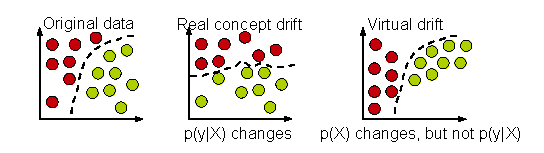
\includegraphics[height=0.15\textheight]{images_cropped/gama_survey_cd_fig1}
	\caption{Illustration from~\cite{gama2014survey} depicting real and virtual concept drift phenomena. Circles represent instances $x_i$, different colors - classes, dashed line is a decision boundary. }\label{fig:fig1_gama_survey_cd}
\end{figure}

\begin{figure}[htb!]
	\centering
	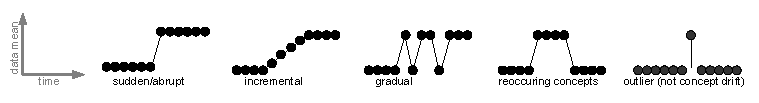
\includegraphics[width=0.9\textwidth]{images_cropped/gama_survey_cd_fig2}
  \caption{Changes between concepts can be gradual or abrupt~\cite{gama2014survey}}\label{fig:fig2_gama_survey_cd}
\end{figure}

\begin{figure}[htb!]
	\centering
	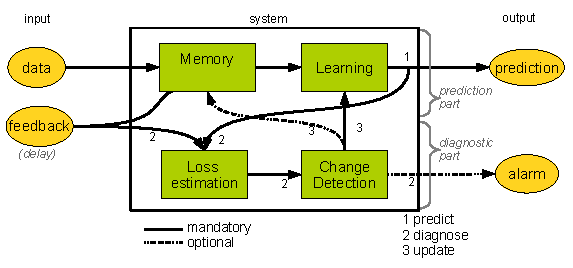
\includegraphics[width=0.9\textwidth]{images_cropped/gama_survey_cd_fig3}
  \caption{A generic schema for an online adaptive learning algorithm (from~\cite{gama2014survey})}\label{fig:fig3_gama_survey_cd}
\end{figure}

\begin{figure}[htb!]
	\centering
	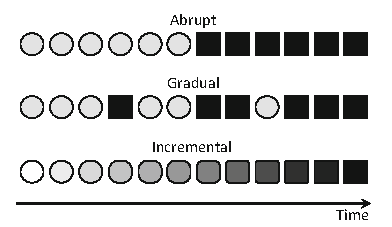
\includegraphics[height=0.15\textheight]{images_cropped/krop_souza_cd_speed}
	\caption{Illustration from~\cite{SouzaChallenges2020}: illustration of three types of concept drift with regard to speed of change.}\label{fig:souza_cd_speeds}
\end{figure}


\section{The link between change detection and concept drift}

Concept drift and change detection in time series are closely related problems.
\textit{Concept} is a set of contiguous examples where the distribution is stationary.
In~\cite{gama2004learning} authors proposed a method to detect changes in the distribution of the training examples.
The drift detection method works by monitoring the online error-rate of a model.

The next paragraph is from~\cite{gama2004learning}.
Suppose a sequence of examples $(x_i, y_i)$.
For each example the model predicts $\hat y_i$ that can be True or False.
For a set of examples the error is a random variable from Bernoulli trials.
The probability of the number of errors for $n$ examples is given by the Binomial distribution.
Probability to observe False for an example $x_i$ is $p_i$ with the standard deviation $s_i=\sqrt{p_i(1-p_i)/i}$.
Statistical decision theory guarantees that while the class distribution of the examples is stationary, the error rate of the learning algorithm ($p_i$) will decrease when $i$ increases.
A significant increase in the error rate of the model implies a change in the class distribution.

SINE1~\cite{gama2004learning} artificial dataset.
In the first concept all points below the curve $y=sin(x)$ have label 1, and all points above have label 0.
After the concept change labelling is reversed.

Machine Learning models learn the relation between input data $x$ and target
variable $y$ by approximating a joint distribution $p(x,y)$.  Model performance
degrades when learned underlying data distribution changes.  Therefore concept
drift can be detected by monitoring change points in model's output performance
statistics.

\section{Example: Insects}
% https://sites.google.com/view/uspdsrepository
% pass: DMKD2018
~\cite{SouzaChallenges2020}


\section{Example: Arima concept drift example}
% https://otexts.com/fpp2/AR.html
Let's consider AR(1) process.
Autoregressive-integrated moving average (ARIMA)~\cite{box2015time} model models stationary processes when the process remains in equilibrium about a constant mean level.
Forecasts are usually needed over a period known as lead time $l$.

In the autoregressive model
the current value is expressed as 
let $\tilde{y}_t = y_t - \mu$
Equation~\ref{eq:ar_proc} is autoregressive (AR) process of order $p$
\begin{equation}\label{eq:ar_proc}
  y_{t} = c + \phi_{1}y_{t-1} + \phi_{2}y_{t-2} + \dots + \phi_{p}y_{t-p} + \varepsilon_{t},
\end{equation}
where $\varepsilon_{t}$ is a white noise. 
\begin{equation}\label{eq:ma_proc}
  y_{t} = c + \varepsilon_t + \theta_{1}\varepsilon_{t-1} + \theta_{2}\varepsilon_{t-2} + \dots + \theta_{q}\varepsilon_{t-q}
\end{equation}
for stationary processes constrains are~\cite{hyndman2018forecasting} 
\begin{itemize}
  \item for AR(1) $-1 < \phi_1 < 1$
  \item for AR(2) $-1 < \phi_2 < 1, \phi_1+\phi_2 <1, \phi_2-\phi_1 < 1$
\end{itemize}
\begin{figure}[!htb]
	\centering
	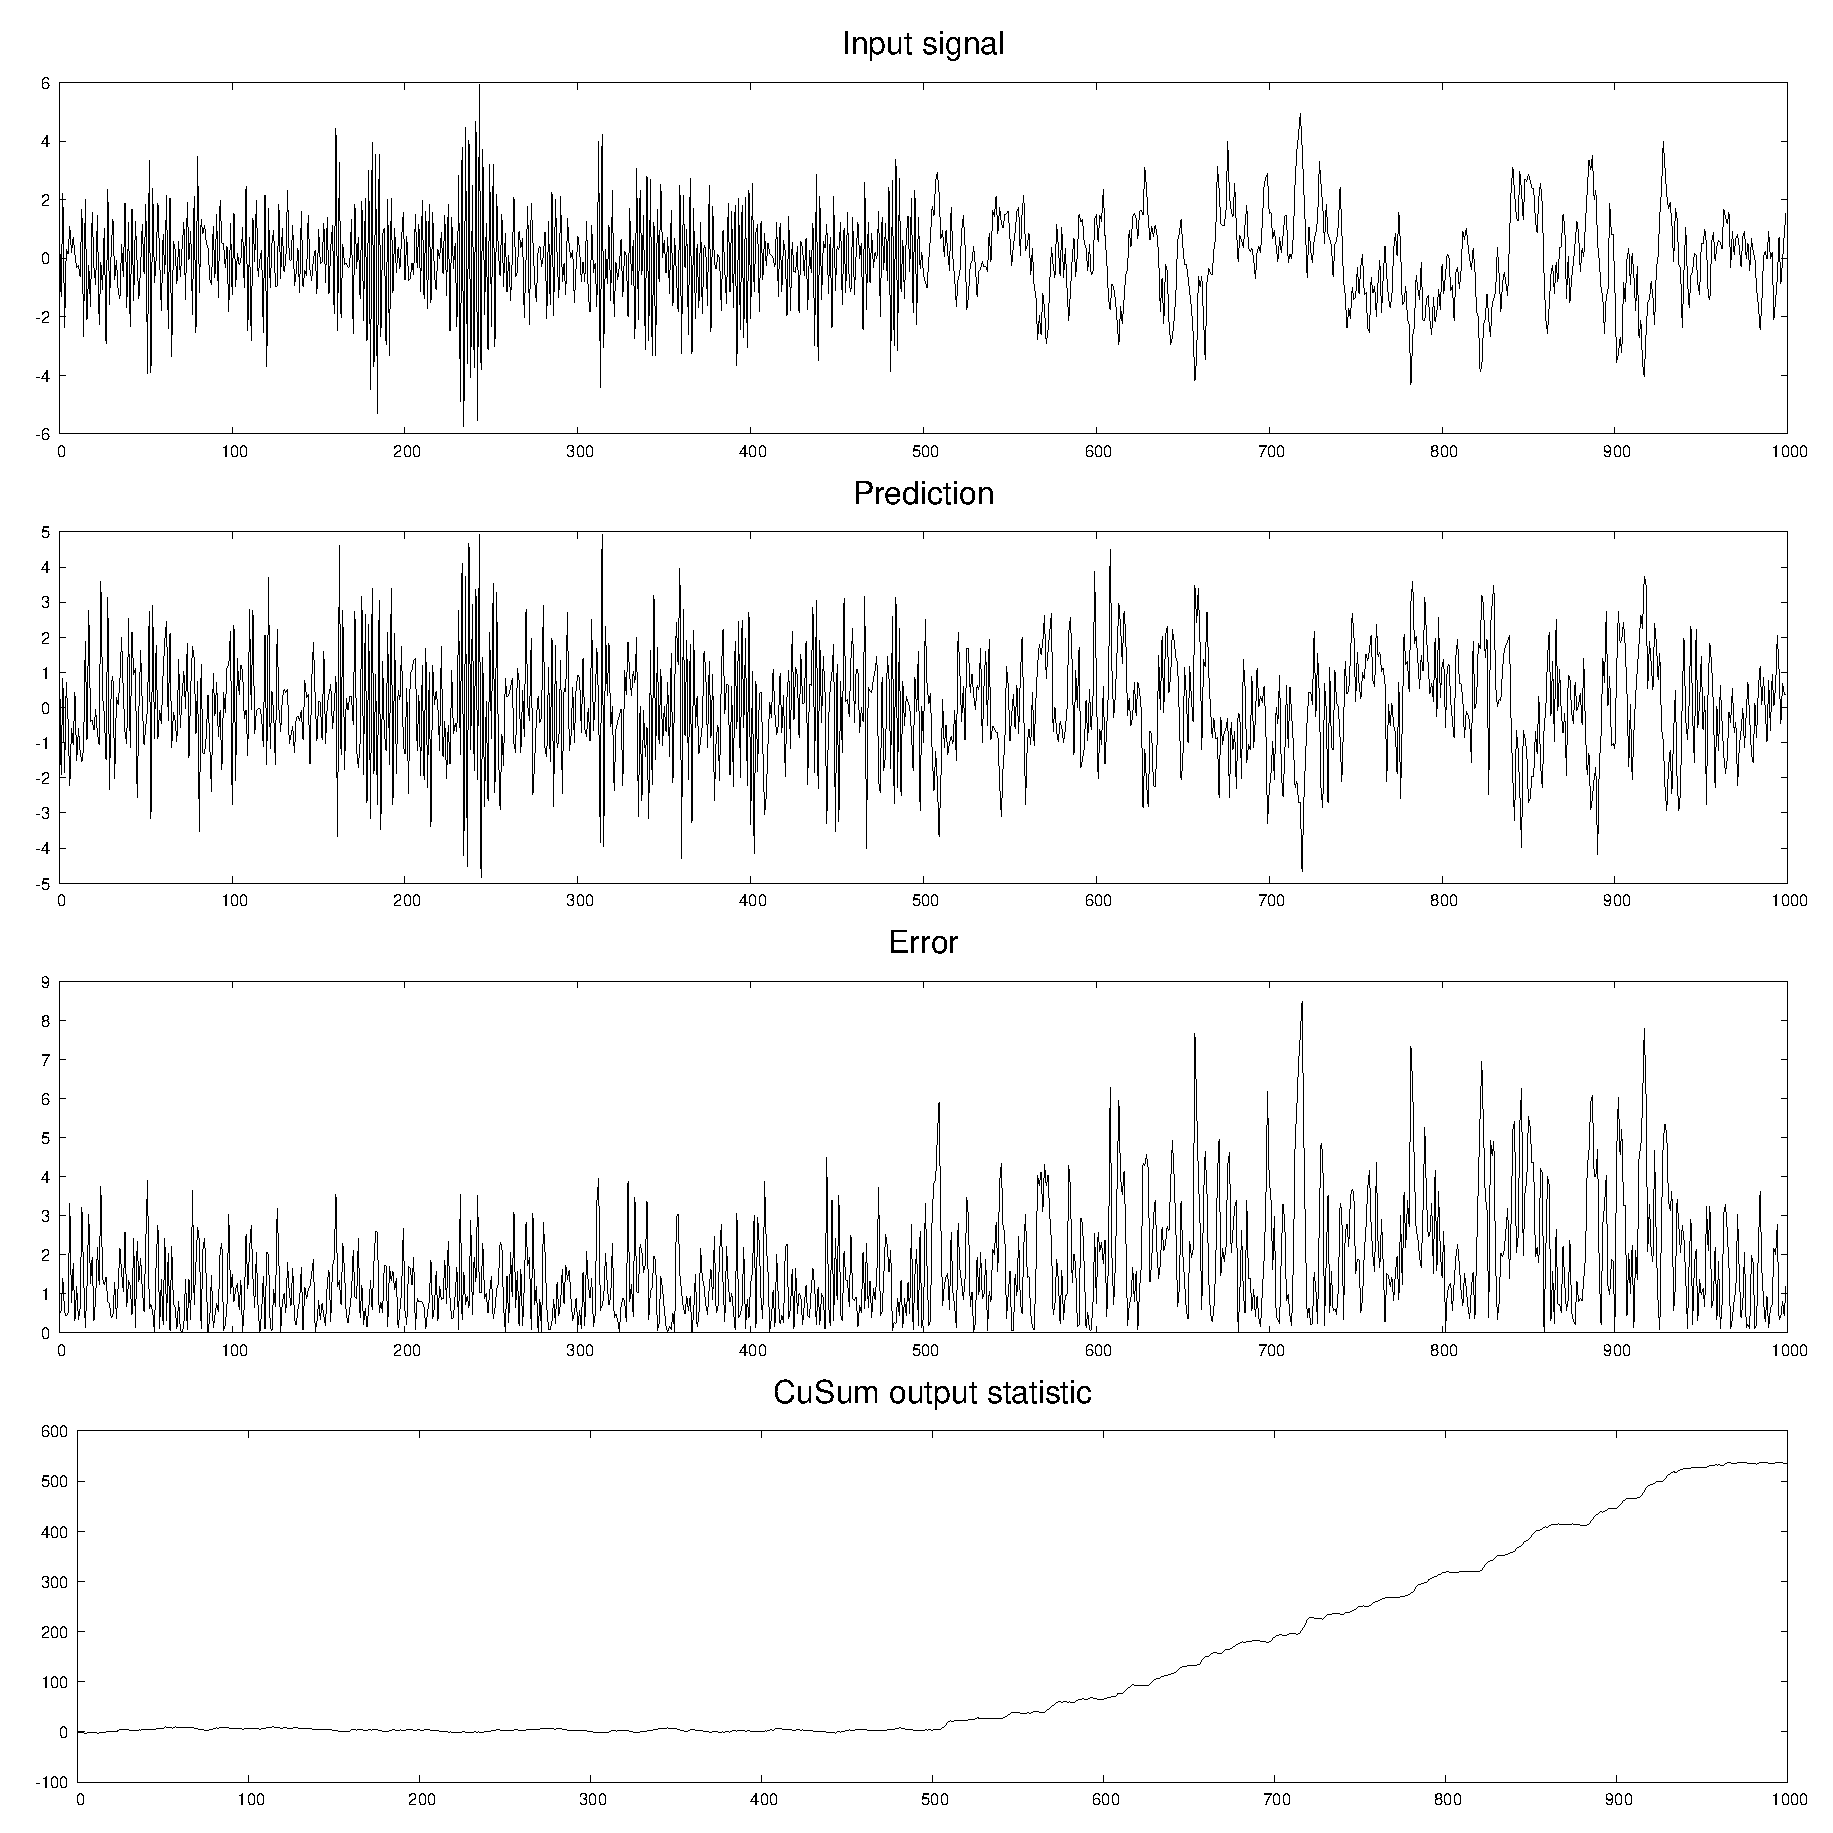
\includegraphics[width=0.9\textwidth]{images/arima_cd_example}
	\caption{Arima concept drift example.
		Two $AR(1) $ processes.
		First and second halfs of the signal is generated by the $AR(1)$ process
	}\label{fig:arima_cd_example}
\end{figure}
% \tilde{y}_t = \phi_1 \tilde{y}_{t-1} + \phi_2 \tilde{y}_{t-2} + \dots + \phi_p \tilde{y}_{t-p} + a_t
%where $a_t \sim \mathcal{N}(\mu, \sigma_a)$.


\section{Example: ELEC2}
The electricity market data set ELEC2~\cite{harries1999splice, gama2004learning} is widely used for testing adaptive learning techniques.
It should be noted however that it is not clear if there is a concept drift in the dataset~\cite{zliobaite2013good}. 
%https://www.openml.org/d/151
%Electricity is a widely used dataset described by M. Harries and analyzed by J. Gama (see papers below). This data was collected from the Australian New South Wales Electricity Market. In this market, prices are not fixed and are affected by demand and supply of the market. They are set every five minutes. Electricity transfers to/from the neighboring state of Victoria were done to alleviate fluctuations.
%
The dataset (originally named ELEC2) contains 45,312 instances dated from 7 May 1996 to 5 December 1998. 
Each example of the dataset refers to a period of 30 minutes, i.e. there are 48 instances for each time period of one day. 
Each example on the dataset has 5 fields, the day of week, the time stamp, the New South Wales electricity demand, the Victoria electricity demand, the scheduled electricity transfer between states and the class label. 
The class label identifies the change of the price (UP or DOWN) in New South Wales relative to a moving average of the last 24 hours (and removes the impact of longer term price trends). 
%
%The data was normalized by A. Bifet.
%
%### Attribute information  
%* Date: date between 7 May 1996 to 5 December 1998. Here normalized between 0 and 1
%* Day: day of the week (1-7)
%* Period: time of the measurement (1-48) in half hour intervals over 24 hours. Here normalized between 0 and 1
%* NSWprice: New South Wales electricity price, normalized between 0 and 1
%* NSWdemand: New South Wales electricity demand, normalized between 0 and 1
%* VICprice: Victoria electricity price, normalized between 0 and 1
%* VICdemand: Victoria electricity demand, normalized between 0 and 1
%* transfer: scheduled electricity transfer between both states, normalized between 0 and 1
\begin{figure}[!htb]
	\centering
	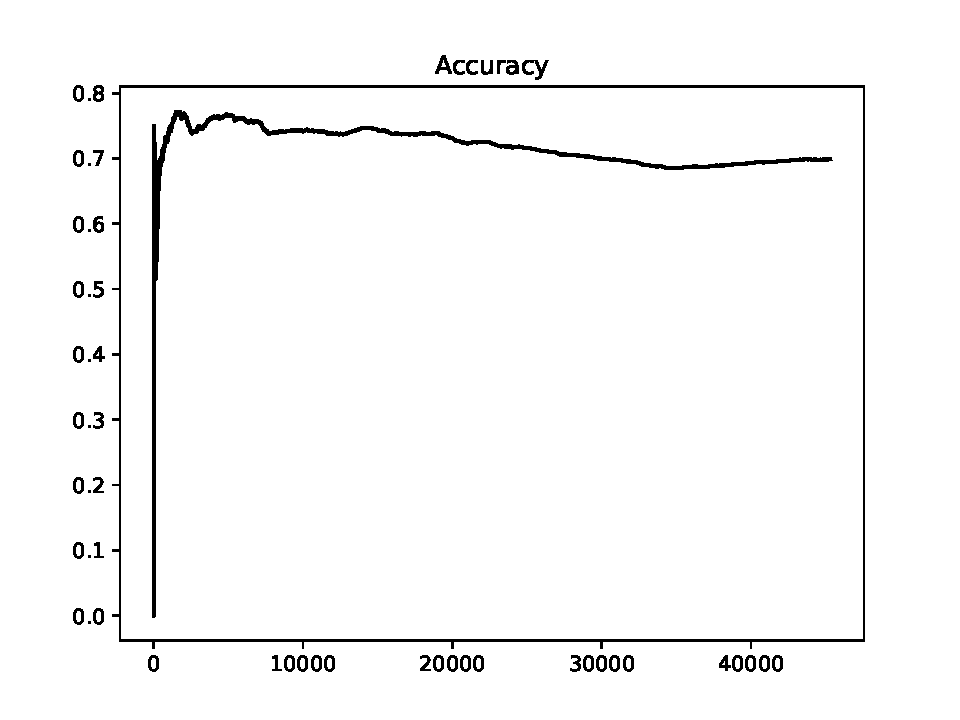
\includegraphics[width=0.9\textwidth]{images/cd_example_elec2.pdf}
	\caption{Elec2 dataset}\label{fig:elec2}
\end{figure}

\section{Example: SINE1}
\begin{figure}[!htb]
	\centering
	\includegraphics[width=0.9\textwidth]{images/cd_example_sine1}
	\caption{SINE1 artificial dataset. 
		Before concept drift (CD) all points above the curve $y=\sin(x)$ are classified as positive.
After CD - as negative.	
}\label{fig:sine1}
\end{figure}

\section{Example: CFB signal}

Why adaptive with detection is better than just adaptive?

Outliers in CFB cause increased calculated prediction error when predicted value is according to the linear trend. 

In continuous update model is being re-trained after
using window of width $w$ $(x_{t-w}, \dots, x_{t})$

In case of adaptive learning with change detection model is re-trained in a sliding window but if change is alarmed at moment $t^c$ then model uodates using 

If Pccf is available then 

In the CFB signal there are outliers between concept drifts.
We run a linear regression model trained using sliding window.
The model predicts $x(t)$ given $(x_{t-w}, \dots, x_{t-1})$ for $t in (1, \dots, n-1)$.
If change is alarmed due to outlier then ..


\begin{figure}[!htb]
	\centering
	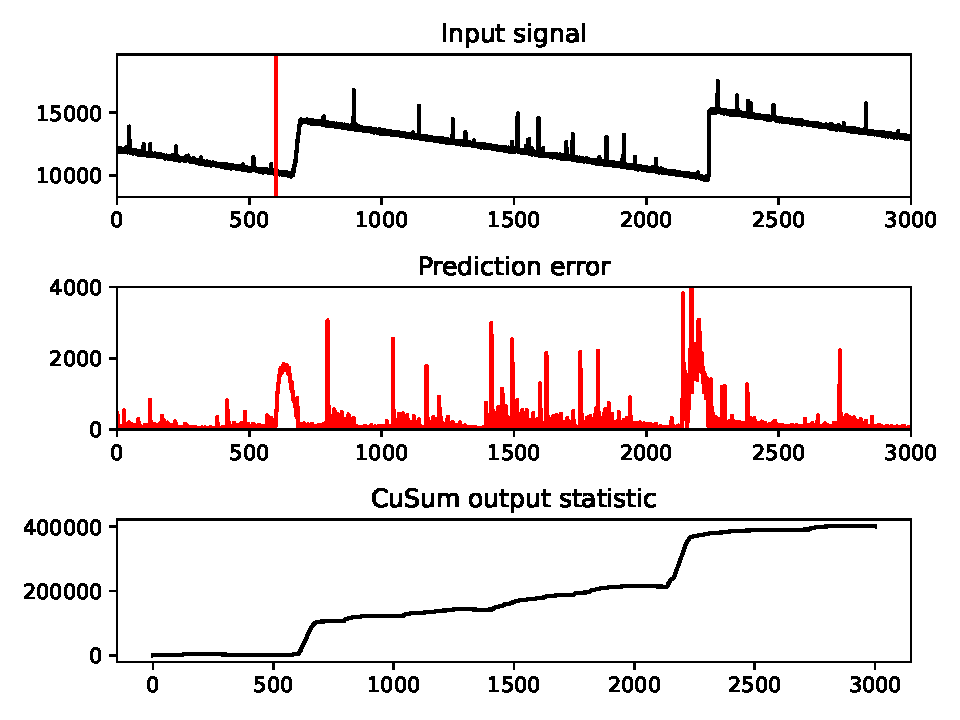
\includegraphics[width=0.9\textwidth]{images/boiler_fixed_train}
	\caption{CFB boiler signal.
Linear regression model is trained using first 600 observations (vertical red line).	
}\label{fig:boiler_fixed_train}
\end{figure}

\section{Change detection problem}

On-line change detection in time series data is an old practical problem with the roots in the problem of statistical quality control~\cite{basseville1993detection,NISTbook}.
Walter A. Shewhart invented control charts in 1924 while working on the problem of statistical quality control to improve reliability of telephone transmission systems. 
Quality control example: $X$ is a set of sensor readings and $y=good$ is a quality of the produced item. 
Offline and online. 
In offline learning all training data is available during training. 
In online learning the data is processed sequentially from data streams.
Model is being updated as more data arrives. 
Data evolve over time in dynamically changing environments.

\begin{figure}[!htb]
	\centering
	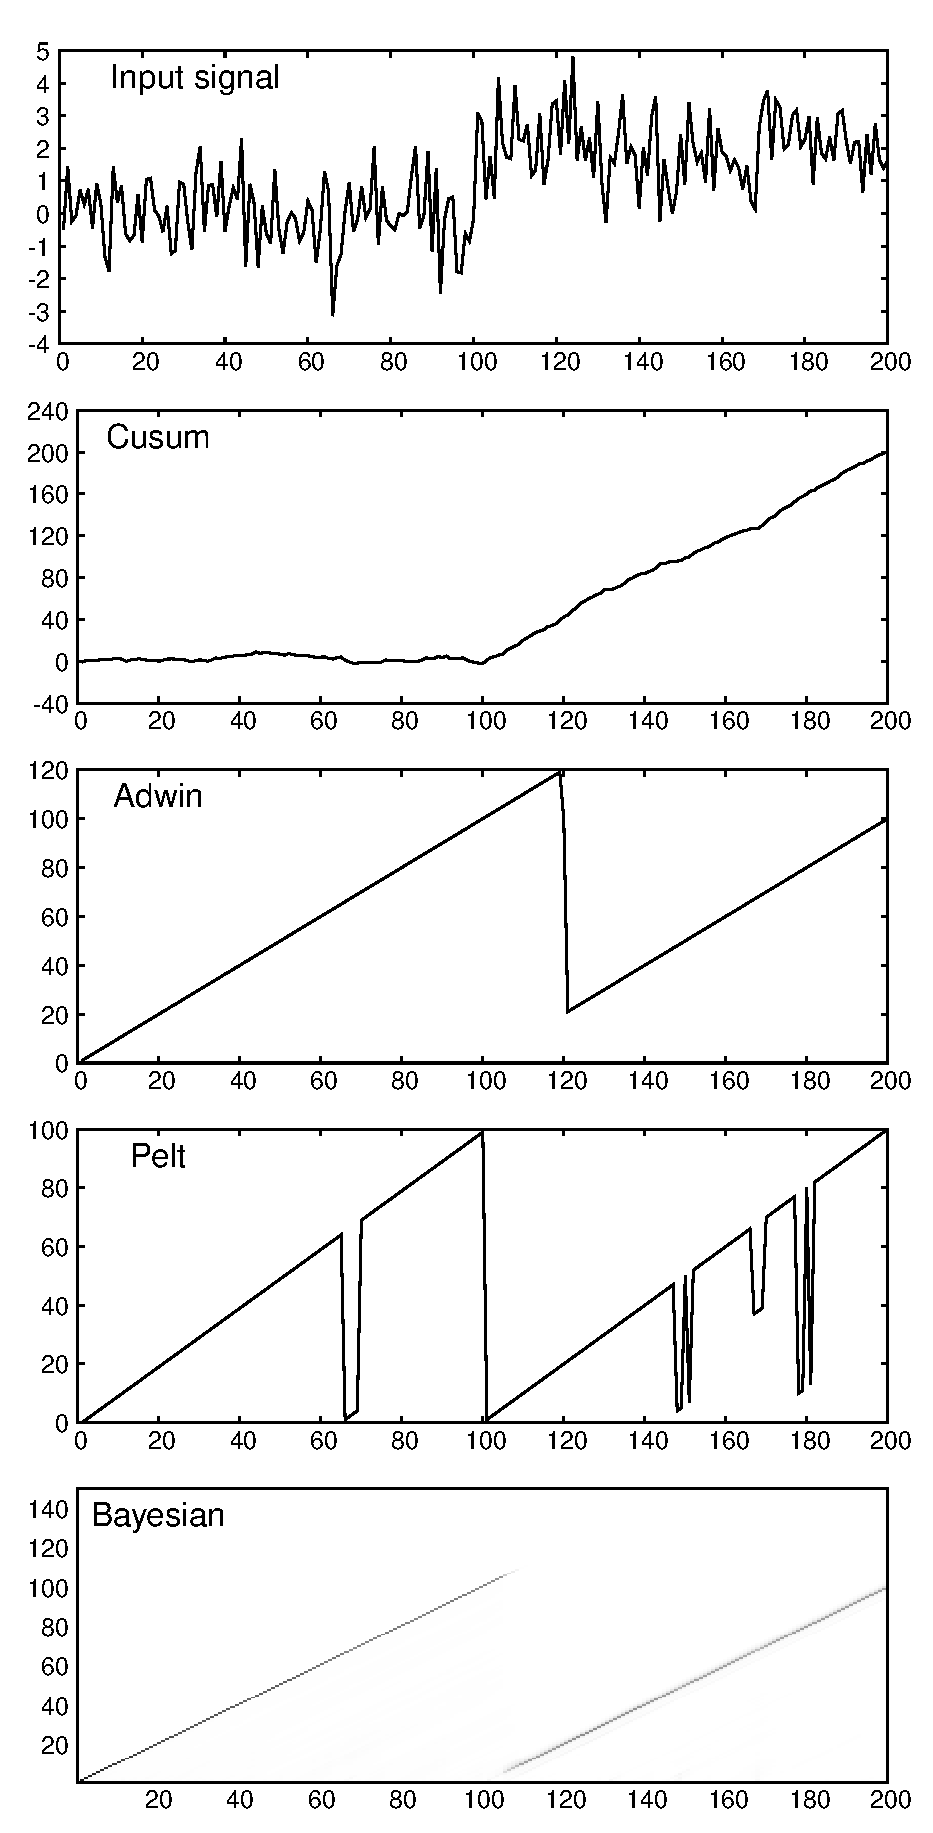
\includegraphics[height=0.9\textwidth]{images/detectors_output_stats}
	\caption{All}\label{fig:all_detectors_stats}
\end{figure}

\section{Detectors}
\subsection{Adwin}
Adwin was proposed in~\cite{bifet2007learning}.
Confidence value $\delta \in (0,1)$
Equation\ref{eq:adwin_ecut}.
\begin{equation}\label{eq:adwin_ecut}
	\epsilon_{\text{cut}} = \sqrt{\frac{2}{m} \cdot \sigma_W^2 \cdot \ln{\frac{2}{\delta^\prime}}} + \frac{2}{3m} \ln{\frac{2}{\delta^\prime}}
\end{equation}
Algorithm\ref{alg:adwin}
\begin{algorithm}[!h]
	\begin{algorithmic}[1]
		\Function{Adwin}{}
		\State Initialize window $W$
		\For{t $\in$ [1, n]}
		\State $W=W \cup x_t$\Comment{Add $x_t$ to the head of $W$} 
		\Repeat
		\State Drop elements from the tail of $W$
		\Until{$|\mu_{W_0} - \mu_{W_1}|\geq \epsilon_{\text{cut}}$ holds for every split of $W=W_0\cdot W_1$}
		\EndFor
		\EndFunction
	\end{algorithmic}
	\caption{Adwin pseudocode \cite{bifet2007learning}}\label{alg:adwin}
\end{algorithm}
\begin{figure}[!htb]
	\centering
	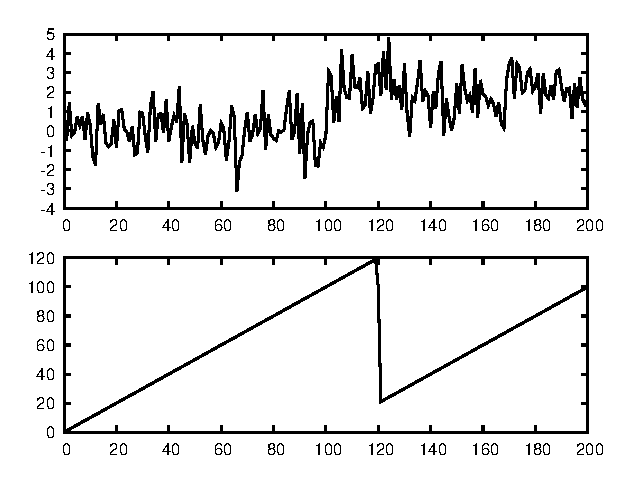
\includegraphics[width=0.9\textwidth]{images/example_output_adwin.eps}
	\caption{ADWIN}\label{fig:adwin_output_example}
\end{figure}

\subsection{Pelt method}

Offline detector used in online settings in ~\cite{marrero2013aclac}.
~\cite{killick2012optimal}
Pelt method is based on a common approach of  minimising a cost function over possible numbers and locations of change points.
Pelt is based on~\cite{jackson2005algorithm}, but involves a pruning step reducing the computational cost but not affecting exactness of the resulting segmentation.
Dynamic programming~\cite{bellman1966dynamic}.

Time interval $I$.
Ordered sequence of data $y_{1:n}=(x_1,\dots,y_n)$.
A partition $P$ of an interval $I$ is a set of blocks is defined  by change points $\tau_{1:m}=(\tau_1, \dots, \tau_m)$.
Each change point is an integer between 1 and $n-1$.
We define $\tau_0=0$ and $\tau_{m+1}=n$.
$m$ change points split the data into $m+1$ segments, $i$-th segment is $y_{\tau_{i-1} : \tau_i}$.
For example, if there is one changepoint $\tau_1$ the segments are $B_1=y_{\tau_0:\tau_1}$ and $B_2=y_{\tau_1:\tau_2}$ where $\tau_2 \equiv n$.
The goal is to find an optimal partition by minimising the cost function defined by Equation\ref{eq:cost_function}
\begin{equation}\label{eq:cost_function}
	\sum_{i=1}^{m+1} [ C(B_i) ] + \beta f(m),\: \text{where } B_i \equiv y_{\tau_{i-1} : \tau_i}
\end{equation}
where $\beta f(m)$ is a regularization term to prevent overfitting.
Commonly used cost functions are twice the negative log likelihood~\cite{guyon1999underfitting,chen2011parametric},
quadratic loss and cumulative sums~\cite{inclan1994use, rigaill2010pruned}.
The most common choices for the regularization term are usually $\beta f(m) = \beta m$.
Examples are Akaike's Information Criterion (AIC\cite{akaike1974new}) $\beta=2p$ and Schwartz Information Criterion (BIC\cite{schwarz1978estimating}) ($\beta = p \log{n}$) where $p$ is the number of additional parameters introduced by adding a new changepoint.
Dynamic programming optimal segmentation is based on the next principle of optimality
\begin{theorem}
Let $P^{\text{max}}$ be an optimal optimal partition of $I$
\end{theorem}

\begin{algorithm}[!h]
	\begin{algorithmic}[1]
		\Function{pelt}{$Y$, $\sigma$, $C(s,t)$}
		\State n = length($Y$)
		\State $F$ = zeros(n)\Comment{Optimal segmentation costs till $t$}
		\State $F[0] = - \log(n)$
		\State previous\_changes\_opt = zeros[n]\Comment{Optimal previous change location}
		\For{t $\in$ [2, n]}
		\State previous\_changes\_possible = $1,\dots,t-1$
		\State i = 0
		\For{s $\in$ previous\_changes\_possible}
		\State i += 1
		\State segmentation\_costs[i] = $C(s, t)$
		\EndFor
		\State costs = $F[\text{previous\_changes\_possible}]$ + segmentation\_costs + $\log(n)$
		\State $F[t+1] = min(\text{costs})$
		\State $\text{previous\_changes\_opt}[t] = \text{previous\_changes\_possible}[argmin(\text{costs})]$
		\EndFor
		\State detections = $\text{fn\_extract\_detections(previous\_changes\_opt)}$
		\EndFunction
	\end{algorithmic}
	\caption{Pelt algorithm}\label{alg:pelt}
\end{algorithm}
\begin{figure}[!htb]
	\centering
	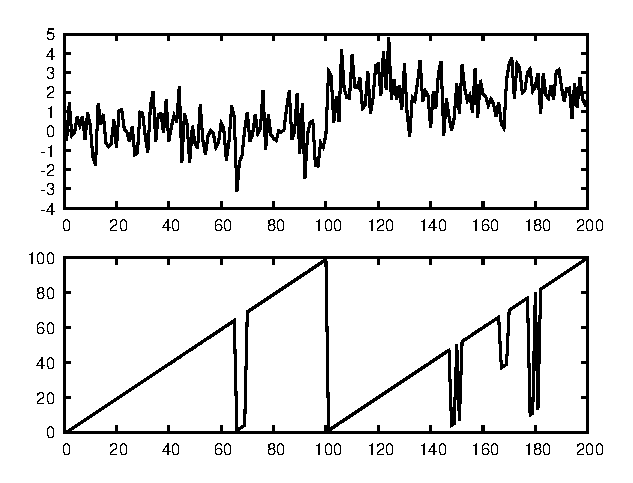
\includegraphics[width=0.9\textwidth]{images/example_output_pelt.eps}
	\caption{PELT}\label{fig:pelt_output_example}
\end{figure}

\subsection{Bayesian detector}

\cite{adams2007bayesian}
BD detector works by recursively estimating posterior probability distribution $P(r_t | \pmb{x}_{1:t}, \theta)$ of the \textit{run length} variable $r_t$ which is a time since the last changepoint.
Changepoint is an event when
\begin{equation}
	\operatorname*{arg\,max}_{r_t} P(r_t | \pmb{x}_{1:t}, \theta) = 0
\end{equation}
%$r_t = 0$
Every time a new measurement $x_t$ is observed the \textit{posterior} distribution is recalculated using the Bayes` theorem to update parameters of the distributions used to model data
\[
(r_t | \pmb{x}_{1:t}) = \frac{P(r_t, \pmb{x}_{1:t})}{P(\pmb{x}_{1:t})}
\]
and the law of total probability
%$P(x) = \sum_{y} P(x|y) p(y)$
\begin{equation}
	P(r_t|\:\LargeCdot) = \sum_{r_{t-1}} P(r_{t} | \: r_{t-1},\:\LargeCdot) \: P(r_{t-1}|\:\LargeCdot)
\end{equation}
to take into account values from all the runs in the past.
The \textit{prior} probability of the change $P(r_t=0|t)$ in BD detector is specified using the constant-value hazard rate $h$ which is a prior probability to observe a change and which is supposed to be known before the change detection process starts.
\begin{figure}[!htb]
	\centering
	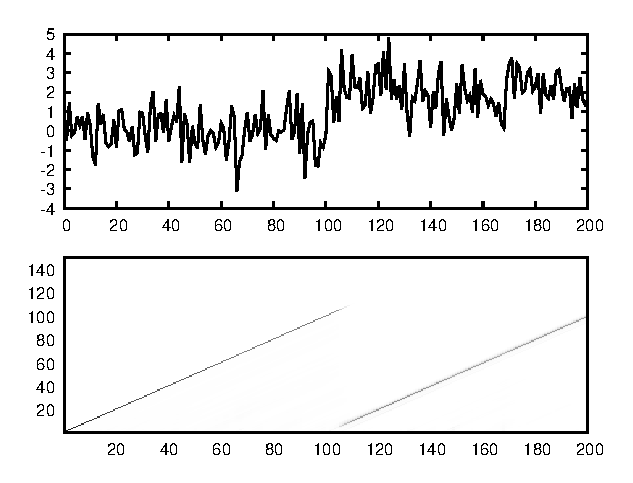
\includegraphics[width=0.9\textwidth]{images/example_output_bayes.eps}
	\caption{Bayes}\label{fig:bayes_output_example}
\end{figure}

\subsection{CUSUM detector}

In this section, we describe the CuSum~\cite{Page1954} detector and its output statistic properties important for measuring performance metrics in static and dynamic settings.
Changes in the stream of measurements reflect dynamics of observed phenomenon happening in time.
Therefore, strictly speaking, any change is a gradual process.
In this paper, for simplicity, we refer to change points and to detections as individual time moments as if change would have happen instantly. If change is gradual and spans time interval then it can be reduced to a single time moment by considering the start or end of the change event~\footnote{Gradual change may become represented as an abrupt change in the time series also due to the sampling rate of measurements}.
Change points in the signal are characterized by the time moment when they happened and by the corresponding mean shift value in the signal.
\begin{definition}
	Change point is a time moment $t^c$ when statistical properties of the data stream change significantly accordingly to a predefined criteria.
\end{definition}
\begin{definition}
	Detection is a time moment $t^d$ when a detector alarms a change.
\end{definition}
For example, if $x_i \sim \mathbb{N}(\mu_1, \sigma)$ for $i < k$ and $x_i \sim \mathbb{N}(\mu_2, \sigma)$ for $i \geq k$,
then we say that a change point occurred at time moment $t_k$, i.e. $t^{\text{c}}_{k} \equiv t_k$.
In general, detection can usually be alarmed before or after a change point.
If $t^{\text{d}}_k > t^{\text{c}}_k$, then change is detected with the delay $t^{\text{d}}_k - t^{\text{c}}_k$.
%TOMMI: Can we give definition like below? I.e. to say that ALL too-early alarms are false alarms?
If $t^{\text{d}}_k < t^{\text{c}}_k$ then detection $t^{\text{d}}_k$ is a false alarm (FA).

As an input, CuSum detector receives time series of observations~\ref{eq:input_ts} usually taken at constant sampling rate.
\begin{equation}\label{eq:input_ts}
	(x_i)_{i=1}^{N} \equiv (x_1, x_2, \dots, x_N)
\end{equation}
taken at corresponding time moments $(t_i)_{i=1}^N$.
Observations and time moments are enumerated by index $i$ mapping $t_i$ to observations $x_i$ and vice versa.
CuSum works through a sequential calculation of the output statistic as follows
% Cusum rule: https://www.itl.nist.gov/div898/handbook/pmc/section3/pmc323.htm
\begin{align}
	S_0 &= 0 \nonumber \\
	S_{n} &= \max (0, S_{n-1} + x_n - \mu_0 - k )\label{eq:cusum_scheme}.
\end{align}
% Detections are alarmed at time moments when Cusum's output statistic exceeds a threshold value $h$.
Detections are alarmed at time moments when $S_{t+1} > h$, i.e. when output statistic exceeds a threshold value $h$.
In \eqref{eq:cusum_scheme}, $\mu_0$ is the estimate of the in-control state signals' mean value.
The parameter $k$ is called allowance value and it depends on the level of mean shift $\delta=\mu_2-\mu_1$ that we aim to detect.

\begin{algorithm}
	% class Detector
	\begin{algorithmic}[1]
		%\Function{CusumSingle}{$X$, $h$, $\text{PCCF}$}\Comment{Single changepoint detection}
		%\State n=length($X$)
		%\State stat=zeros(n)
		%\State stat[0]=X[0] - $\mu_0$
		%\For{t $\in$ [1,n]}
		%\State stat[t] = stat[t-1]+X[t]-$\mu_0$
		%\If{(not PCCF) or (PCCF and WithinRoi()) }
		%\If{$|stat[t]| > h$}
		%\State \Return (t, stat) \Comment{Alarm CDE}
		%\EndIf
		%\EndIf
		%\EndFor
		%\State \Return (nan, stat)\Comment{Return missing value for CDE}
		%\EndFunction  
		%\\
		\Function{CusumMutli}{$X$, $h$, $\text{PCCF}$}\Comment{Sequential/multi- changepoint detection}
		\State n = length(Signal)
		\State detections = [ ]
		\For{t $\in$ [1,n]}
		%\While{$t <n$}
		\State UpdateMu(Signal[t])
		\State UpdateCusumStatistic()
		\If{PCCF and EnteredRoi()}
		\State NextRoiIndex $\mathrel{{+}{=}} 1$
		\EndIf
		%\Comment{If we don't use Pccf or we use Pccf and we are inside ROI}
		\If{(not PCCF) or (PCCF and WithinRoi()) }
		\If{$|stat[t]| > h$}
		\State detections.append(t) \Comment{Collect CDEs}
		\State ResetDetector()
		\EndIf
		\EndIf
		%\State t $\mathrel{{+}{=}} 1$
		%\EndWhile
		\EndFor
		\If{len(detections) == 0} \Comment{In case of detecting single change point}
		\State delay = NaN \Comment{Return detection delay NaN if no detection is alarmed}
		\EndIf
		\State \Return detections 
		\EndFunction
		\\
		\Function{UpdateMu}{}\Comment{Running mean value after each CDE}
		\State $\mu_{t}=\frac{k-1}{k} \mu_{t-1} + \frac{x}{k}  $
		\EndFunction
		\\
		\Function{UpdateCusumStatistic}{}\Comment{Update CUSUM statistic}
		\State $\delta = x_t - \mu_t$
		\State $stat[0] = \delta$
		\State $stat[t] = stat[t-1] + \delta \: \forall \: t >0$
		\EndFunction
		\\
		\Function{ResetDetector}{}\Comment{Re-initialize detector after each CDE}
		\State $\mu_t=0$
		\State k=1
		\State $stat[t]=x_t$
		\EndFunction
	\end{algorithmic}
	\caption{Cusum for single and multiple change points detection.}\label{alg:method_code}
\end{algorithm}


\begin{figure}[!htb]
	\centering
	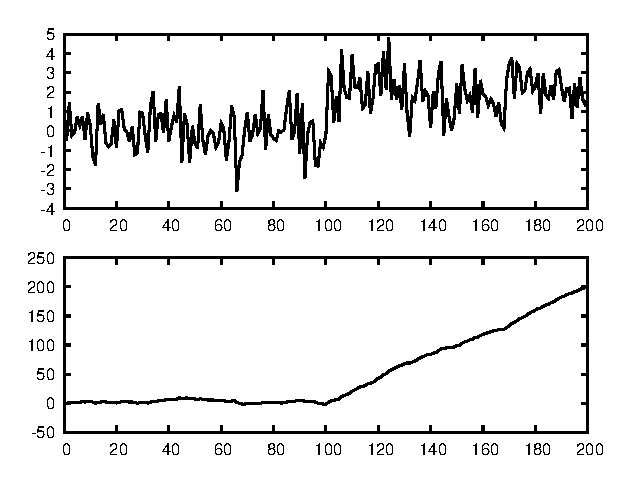
\includegraphics[width=0.7\textwidth]{images/example_output_cusum.eps}
	\caption{CuSum}\label{fig:cusum_output_example}
\end{figure}

\subsection{ARL}

The key performance metric of the CuSum detector is the Average Run Length (ARL), which refers to the expected number of observations before an action is taken, i.e., before the detection is alarmed~\cite{Page1954}.
ARL refers to the FA rate before the change and to the detection delay after the change point.
When the process is in-control, the $ARL_{\delta}$ refers to a FA rate, whereas when the change has happened it refers to the detection delay.
% ARL approximation in Equation~\ref{eq:arl_approximation} is given by~\cite{siegmund2013sequential}.
However, ARL is hard to estimate analytically.
As reported in~\cite{plasse2021streaming}, one of the simplest ARL approximations is given in~\cite{siegmund2013sequential} in a form of the following equation %Equation~\ref{eq:arl_approximation}
\begin{equation}\label{eq:arl_approximation}
	\text{ARL}_{\delta} = \frac{\exp(-2(\delta-k)h') + 2(\delta - k)h' -1}{2 (\delta - k)^2}
\end{equation}
%Here, $\delta=\mu_2-\mu_1$ is the mean shift we aim to detect and
for $h' = h+1.166$.
Figure~\ref{fig:arl} depicts ARL behavior against $\delta$ (left plot) and versus threshold $h$ (right plot).
It is easy to see how ARL refers to both the FA rate and to the detection delay at the same time.
More precisely, smaller values of $\delta$ correspond to fluctuations in the signal and to the larger ARL values, whereas
larger values of $\delta$ indicate change points to be detected.
Not surprisingly, ARL decreases fast when $\delta$ is increased.
It also can be seen that by changeing $\delta$ we increase or decrease ARL value.
We will use this fact later in the experimental part when performing simulations to measure the detection delay by varying ARL values (by changing $\mu_2-\mu_1 \equiv \delta$) for static and dynamic detectors.
%
\begin{figure}[!htb]
	\centering
	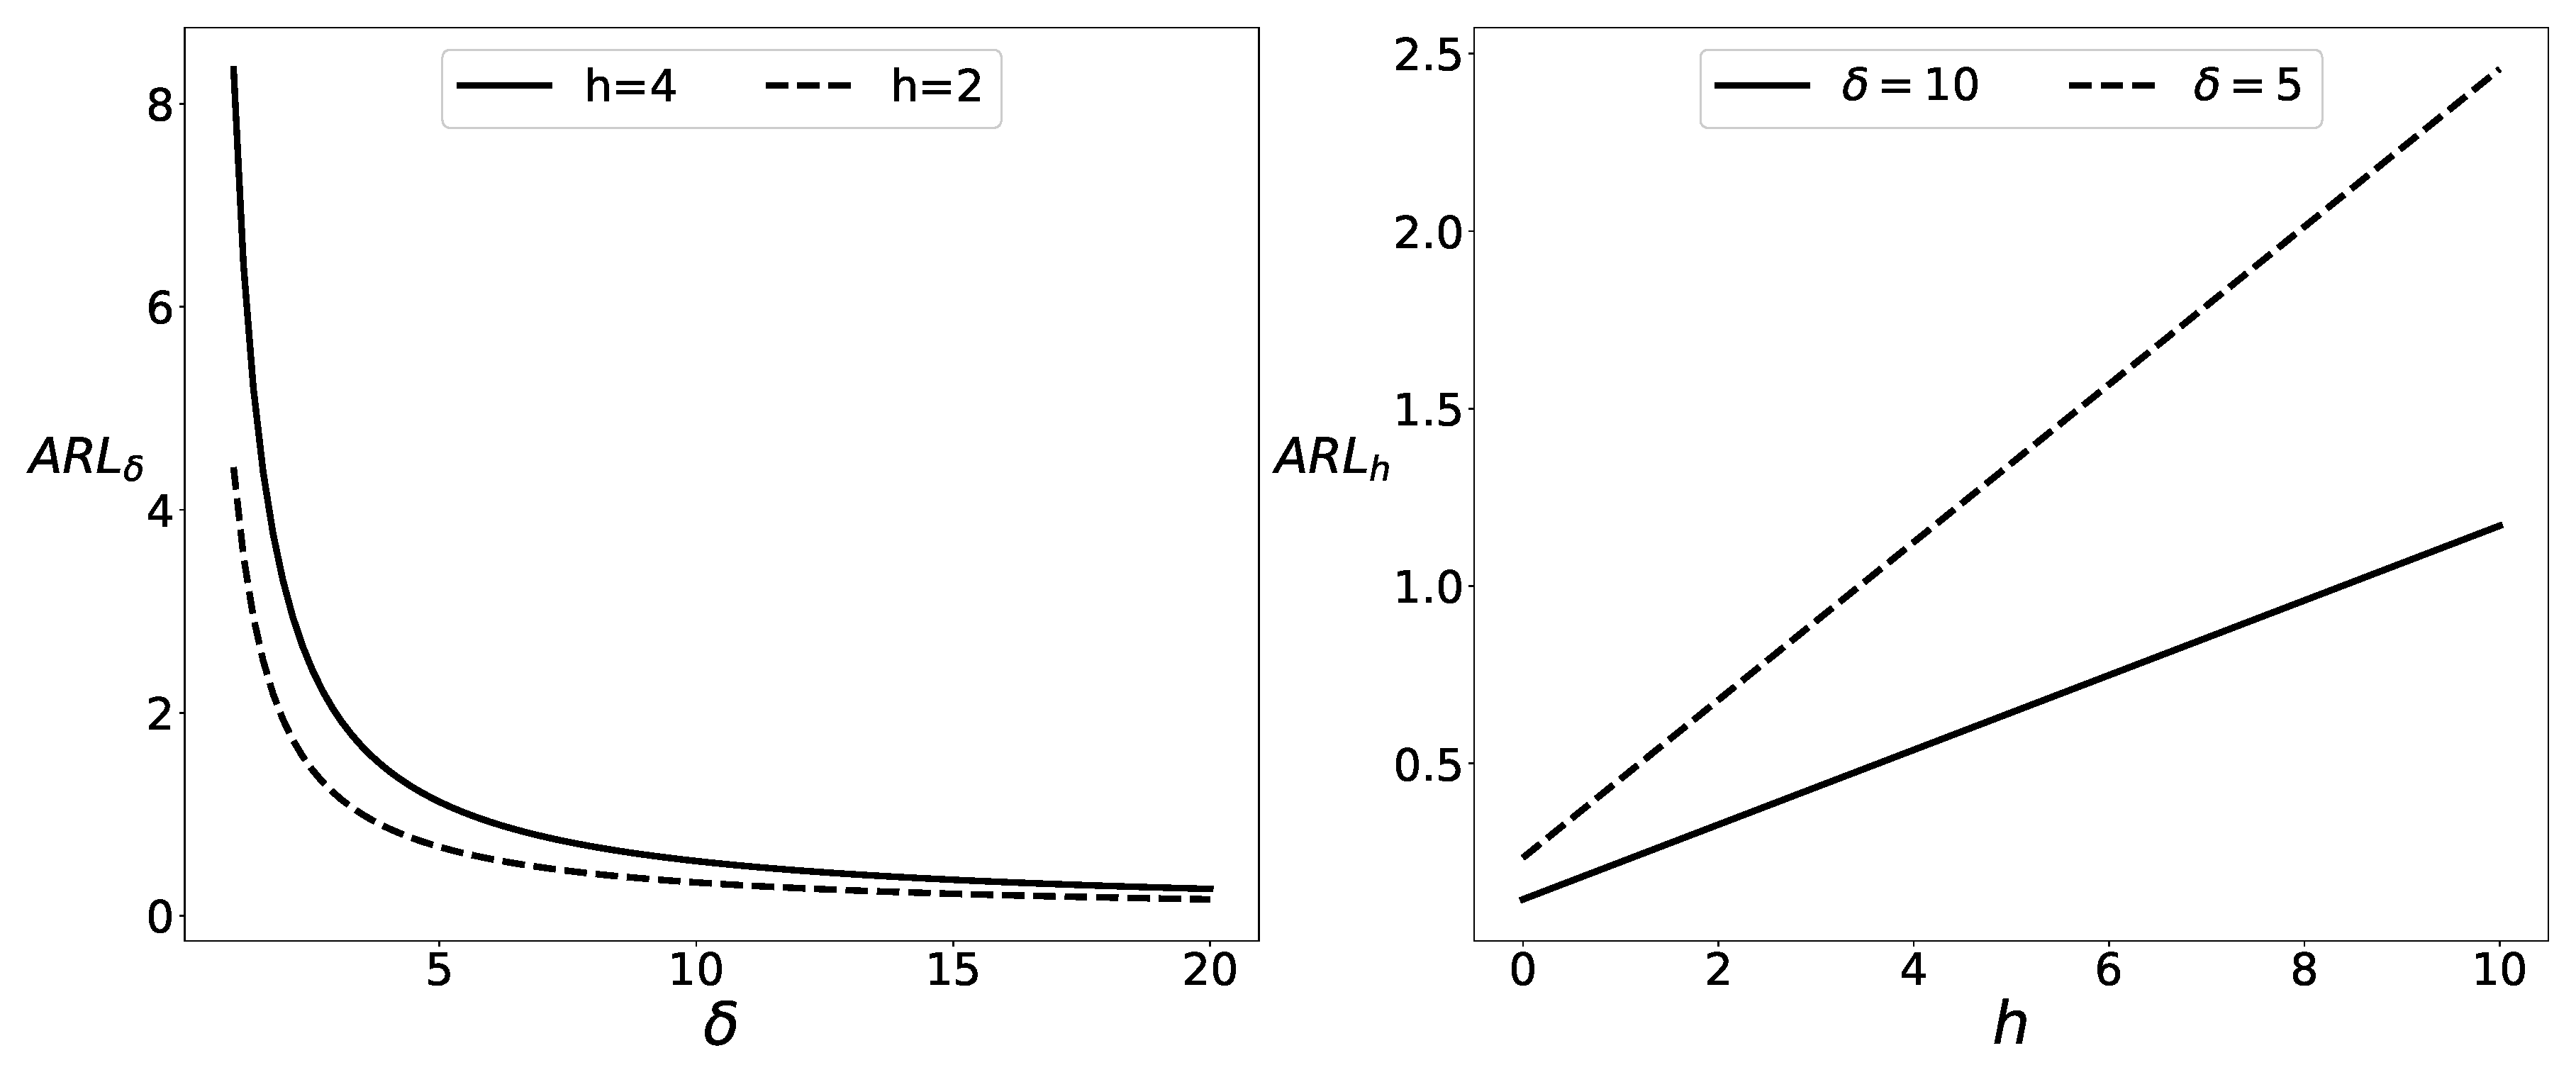
\includegraphics[width=0.9\textwidth]{images_ecmplpkdd/arl.eps}
	\caption{
    The left plot depicts ARL as a function of $\delta = \mu_2-\mu_1$ for two fixed threshold values $h$. The right plot depicts ARL as a function of the threshold value $h$ for two fixed $\delta$ values (Equation~\ref{eq:arl_approximation}).
    Both plots demonstrate that smaller ARL values (and therefore detection delays) correspond to smaller $h$ values. It is obvious for the right plot, on the left plot this fact is depicted by the dashed line for $h=2$ being lower than the solid line for $h=4$.
    %
    Smaller $\delta$ corresponds to the fluctuations in the time series causing false alarms, larger $\delta$ correspond to changes in the level shift which are subject for detection.
    When threshold $h$ is adjusted to smaller values ARL for all $\delta$ values gets smaller (left plot), therefore detection delay is decreased but probability of FA is increased.
    %Left plot depicts that ARL values for the whole range of $\delta$ values are decreased including smaller $\delta$ values corresponding to FA events,i.e.\ average runs between false alarms are also decreased along with the detection delay.
    %
    % Our hypothesis which we investigate experimentally is that by using smaller values of $h$ within prediction intervals and by disregarding detections outside of them we can decrease detection delay and the total number of false alarms despite decreased average runs between them.
}\label{fig:arl}
\end{figure}
%\begin{figure}[!htb]
%	\centering
%	\includegraphics[width=0.7\textwidth]{images/arl3d.eps}
%	\caption{}
%\end{figure}
\begin{figure}[!htb]
% GNUPLOT: LaTeX picture with Postscript
\begingroup
  \makeatletter
  \providecommand\color[2][]{%
    \GenericError{(gnuplot) \space\space\space\@spaces}{%
      Package color not loaded in conjunction with
      terminal option `colourtext'%
    }{See the gnuplot documentation for explanation.%
    }{Either use 'blacktext' in gnuplot or load the package
      color.sty in LaTeX.}%
    \renewcommand\color[2][]{}%
  }%
  \providecommand\includegraphics[2][]{%
    \GenericError{(gnuplot) \space\space\space\@spaces}{%
      Package graphicx or graphics not loaded%
    }{See the gnuplot documentation for explanation.%
    }{The gnuplot epslatex terminal needs graphicx.sty or graphics.sty.}%
    \renewcommand\includegraphics[2][]{}%
  }%
  \providecommand\rotatebox[2]{#2}%
  \@ifundefined{ifGPcolor}{%
    \newif\ifGPcolor
    \GPcolorfalse
  }{}%
  \@ifundefined{ifGPblacktext}{%
    \newif\ifGPblacktext
    \GPblacktexttrue
  }{}%
  % define a \g@addto@macro without @ in the name:
  \let\gplgaddtomacro\g@addto@macro
  % define empty templates for all commands taking text:
  \gdef\gplbacktext{}%
  \gdef\gplfronttext{}%
  \makeatother
  \ifGPblacktext
    % no textcolor at all
    \def\colorrgb#1{}%
    \def\colorgray#1{}%
  \else
    % gray or color?
    \ifGPcolor
      \def\colorrgb#1{\color[rgb]{#1}}%
      \def\colorgray#1{\color[gray]{#1}}%
      \expandafter\def\csname LTw\endcsname{\color{white}}%
      \expandafter\def\csname LTb\endcsname{\color{black}}%
      \expandafter\def\csname LTa\endcsname{\color{black}}%
      \expandafter\def\csname LT0\endcsname{\color[rgb]{1,0,0}}%
      \expandafter\def\csname LT1\endcsname{\color[rgb]{0,1,0}}%
      \expandafter\def\csname LT2\endcsname{\color[rgb]{0,0,1}}%
      \expandafter\def\csname LT3\endcsname{\color[rgb]{1,0,1}}%
      \expandafter\def\csname LT4\endcsname{\color[rgb]{0,1,1}}%
      \expandafter\def\csname LT5\endcsname{\color[rgb]{1,1,0}}%
      \expandafter\def\csname LT6\endcsname{\color[rgb]{0,0,0}}%
      \expandafter\def\csname LT7\endcsname{\color[rgb]{1,0.3,0}}%
      \expandafter\def\csname LT8\endcsname{\color[rgb]{0.5,0.5,0.5}}%
    \else
      % gray
      \def\colorrgb#1{\color{black}}%
      \def\colorgray#1{\color[gray]{#1}}%
      \expandafter\def\csname LTw\endcsname{\color{white}}%
      \expandafter\def\csname LTb\endcsname{\color{black}}%
      \expandafter\def\csname LTa\endcsname{\color{black}}%
      \expandafter\def\csname LT0\endcsname{\color{black}}%
      \expandafter\def\csname LT1\endcsname{\color{black}}%
      \expandafter\def\csname LT2\endcsname{\color{black}}%
      \expandafter\def\csname LT3\endcsname{\color{black}}%
      \expandafter\def\csname LT4\endcsname{\color{black}}%
      \expandafter\def\csname LT5\endcsname{\color{black}}%
      \expandafter\def\csname LT6\endcsname{\color{black}}%
      \expandafter\def\csname LT7\endcsname{\color{black}}%
      \expandafter\def\csname LT8\endcsname{\color{black}}%
    \fi
  \fi
    \setlength{\unitlength}{0.0500bp}%
    \ifx\gptboxheight\undefined%
      \newlength{\gptboxheight}%
      \newlength{\gptboxwidth}%
      \newsavebox{\gptboxtext}%
    \fi%
    \setlength{\fboxrule}{0.5pt}%
    \setlength{\fboxsep}{1pt}%
\begin{picture}(8640.00,8640.00)%
    \gplgaddtomacro\gplbacktext{%
      \csname LTb\endcsname%%
      \put(1055,1901){\makebox(0,0){\strut{}$0$}}%
      \put(1670,1752){\makebox(0,0){\strut{}$0.5$}}%
      \put(2285,1604){\makebox(0,0){\strut{}$1$}}%
      \put(2901,1455){\makebox(0,0){\strut{}$1.5$}}%
      \put(3516,1307){\makebox(0,0){\strut{}$2$}}%
      \put(4131,1158){\makebox(0,0){\strut{}$2.5$}}%
      \put(4746,1010){\makebox(0,0){\strut{}$3$}}%
      \put(5197,1245){\makebox(0,0){\strut{}$0$}}%
      \put(5733,1491){\makebox(0,0){\strut{}$2$}}%
      \put(6269,1736){\makebox(0,0){\strut{}$4$}}%
      \put(6806,1981){\makebox(0,0){\strut{}$6$}}%
      \put(7342,2226){\makebox(0,0){\strut{}$8$}}%
      \put(7879,2472){\makebox(0,0){\strut{}$10$}}%
      \put(1008,3569){\makebox(0,0)[r]{\strut{}$0$}}%
      \put(1008,3965){\makebox(0,0)[r]{\strut{}$50$}}%
      \put(1008,4362){\makebox(0,0)[r]{\strut{}$100$}}%
      \put(1008,4758){\makebox(0,0)[r]{\strut{}$150$}}%
      \put(1008,5154){\makebox(0,0)[r]{\strut{}$200$}}%
      \put(1008,5551){\makebox(0,0)[r]{\strut{}$250$}}%
      \put(1008,5948){\makebox(0,0)[r]{\strut{}$300$}}%
      \put(1008,6345){\makebox(0,0)[r]{\strut{}$350$}}%
    }%
    \gplgaddtomacro\gplfronttext{%
      \csname LTb\endcsname%%
      \put(2604,2003){\makebox(0,0){\strut{}${\delta}$}}%
      \put(5891,1997){\makebox(0,0){\strut{}$h$}}%
      \put(210,4956){\makebox(0,0){\strut{}ARL}}%
    }%
    \gplbacktext
    \put(0,0){\includegraphics[width={432.00bp},height={432.00bp}]{/home/ms314/1/thesis/images/arl3d}}%
    \gplfronttext
  \end{picture}%
\endgroup

\caption{ARL 3D}\label{fig:arl3d}
\end{figure}


\chapter{Recurrency}

Adaptive learning in concept drift.
Predictability of events in the data stream.
~\cite{feller2008introduction}
Sums of independent random variables.
Recurrency is a form of predictability.

\section{Feller}
The basic theory is as follows~\cite{feller2008introduction}.
In a sequence of Bernoulli trials the waiting time up to the first event gas a geometric distribution.
After the first event the process starts anew, and the number of trials between $n$ and $n+1$ th events has the same geometric distribution.
\begin{definition}
	Let $a_1, a_2, \dots, $ be a sequence of real numbers. If 
	\begin{equation}
		A(s) = a_0 + a_1 s + a_2 s^2 + \dots 
	\end{equation}
    converges in some interval $-s_0 < s < s_0 $ , then $A(s)$ is called the generarating function of the sequence $\{a_j\}$. 
\end{definition}

From\cite{wasserman2013all}
\begin{definition}
	The moment generating function MGF, or Laplace transform, of $X$ is defined by
	\begin{equation}
		\psi_X = \mathbb{E}(e^{tX}) = \int e^{tX} dF(x) 
	\end{equation}
where $t$ varies over the real numbers.
\end{definition}

\section{Inter-arrival times modeling}
Basic theory.
\begin{definition}
	A function $\mathbb{P}$ that assigns a real number $\mathbb{P}(A)$ to each event $A$ is a probability distribution if \\
	Axiom 1: $\mathbb{P}(A) \geq 0$ for every $A$\\
	Axiom 2: $\mathbb{P}(\Omega) = 1$\\
	Axiom 3: If $A_1, A_2, \dots $ are disjoint then 
	\begin{equation}
		\mathbb{P} \Big( \bigcup\limits_{i=1}^{\infty} A_i  \Big) = \sum_{i=1}^{\infty} \mathbb{P}(A_i)
	\end{equation}
\end{definition}
Commonly used probability distributions for modelling inter-arrival times.


\chapter{Main results}
~\cite{MaslovSDM2016, MaslovIJCNN2017}

\section{Pccf}~\label{sec:pccf}
If change points are expected to reoccur in the input signal, then this prior information can be used to approximate prediction time intervals, or regions of interest (ROI), where changes are most likely to appear in the future.
Once calculated, and if predictions are correct, then this information can further be used to reduce the false alarm rate of the change detection process, %at the least
and potentially to reduce detection delays too.
FA rate can be decreased just by disregarding detections outside prediction intervals, and the detection delay can be decreased by increasing sensitivity of the detector within prediction intervals.
But, as mentioned, if sensitivity is increased, then probability of FA events will also  increase.
Possibility of decreasing detection delays in the presence of prediction interval is a subject of Experiments section.
We describe next how to calculate prediction intervals for reoccurring change points.

To calculate ROIs for recurrent change points we use a prediction confidence change function (Pccf) proposed in our previous work~\cite{MaslovSDM2016}, where it was calculated using convolutions.
Below we calculate Pccf for several commonly used distributions of inter-arrival times values using moment generating functions, what is a more concise way than when using convolutions.
%~\footnote{we useterms recurrent and reoccurring interchangebly}
% The difference to the previous work is that we calculate Pccf in a concise
% way using moment generating functions and we calculate it for several
% commonly used distributions used for inter arrival time modelling.
%In our previous work we applied threshold value to the calculated probability estimates, but now we found it much more practical just to use equally spaced time moments surrounded by time intervals of a fixed size.
% Probability estimates given by Pccf should be used to assess confidence intervals for predictions and for assessment of how many changes in the future we want to make a prediction for.
Let's start with definitions.
\begin{definition}
	Change points $t_i^{\text{c}}$ are recurrent if their inter-arrival times $t_{i}^{c} - t_{i-1}^{c}$
	% \begin{equation}\label{eq:recurrence_relation}
	%     \Delta_i = t_{i}^{c} - t_{i-1}^{c}
	% \end{equation}
	are i.i.d.\ from the same probability distribution.
	E.g., $t_{i}^{c} - t_{i-1}^{c} \sim \mathbb{N}(\mu, \sigma)$ if $\sigma$ is small.
\end{definition}
%The recurrence relation for recurrent changes is
%\begin{equation} x_{n+1} = x_n + \delta_n \end{equation}
%
Pccf function value at time moment $t_i$ is a probability estimator of recurrent change point to occur at this time moment.
%Pccf function value at time moment $t_i$ is a probability estimation of the event of observing recurrent changepoint at this moment.
%Recurrent changepoints form a sequence determined by recurrence relation given by Equation~\ref{eq:recurrence_relation}.
% $t_{i}^{\text{CHP}} = t_{i-1}^{\text{CHP}} + \Delta_i$.
Pccf can be represented as a matrix~\ref{eq:pccf_matrix} in which elements at row $k$ and column $i$ are probability estimates for change point $t_k^{\text{c}}$ to appear at time moment $t_i$.
\begin{equation}~\label{eq:pccf_matrix}
	\text{PCCF}_{k,i} \equiv P(t_{k}^{\text{c}} = t_i) % \: \forall \:  k, i \in [1,\dots,N
\end{equation}
When calculating ROIs we are interested in total probability of any changepoint occurring at every time moment within prediction horizon.
Since events $t_k^{\text{c}} = t_i$ are disjoint we need to sum up rows of the matrix $\text{PCCF}_{k,i}$
\begin{equation}~\label{eq:pccf_vector}
	\text{PCCF}_{i \in 1:N} = \sum_{k=1}^{N} P(t_k^{\text{c}} = t_i) \equiv \sum_{k=1}^{N} \text{PCCF}_{k,i}
\end{equation}
Further by Pccf we call the vector given by Equation~\ref{eq:pccf_vector}.
%, i.e.  $\sum_{k=1}^{N} P(t_k^{\text{CHP}} = t_i)$.
%	\begin{equation}
%		\text{Any } t_{k}^{\text{CHP}} = t_i
%		% \text{ or } t_{2}^{\text{CHP}} = t   \dots t_{k}^{\text{CHP}} = t
%		%C_1 = t \text{ or } C_2 = t \text{ or } \dots C_n = t
%		\label{eq:events_union}
%	\end{equation}
%Since events $t_k^{\text{CHP}} = t_i$ are disjoint Pccf can be calculated as
%\begin{equation}
%	\sum_{i=1}^{N} \sum_{k=1}^{N} P(t_k^{\text{CHP}} = t_i).
%\end{equation}
%\begin{equation}
%	P\Big(\bigcup\limits_{k=1}^{N} (t_k^{\text{CHP}} = t_i) \Big ) = \sum_{k=1}^{N} P(t_k^{\text{CHP}} = t_i)
%\end{equation} % Wasserman, page5

The sum~\ref{eq:pccf_vector} can be calculated using the notion of moment generating function (Mgf).
As an example, let's assume a Gaussian distribution for inter-arrival times, i.e. $t_{i}^{\text{c}} - t_{i-1}^{\text{c}} \sim \mathbb{N}(\mu, \sigma)$,
with $\sigma$ small enough so that every next change can not happen before the previous one.
For example, if $\mu=60$ seconds and standard deviation is $\sigma=5$ seconds then, using Chebyshev's inequality~\ref{eq:chebyshev_ineq}, probability of
$\mathbb{P}(|t_{i}^{\text{c}} - t_{i-1}^{\text{c}}| \geq 60) \leq 0.007$.
\begin{equation}\label{eq:chebyshev_ineq}
	\mathbb{P}(|X-\mu| \geq k \sigma) \leq \frac{1}{k^2} % %\mathbb{P}(|X-\mu| \geq t) \leq \frac{\sigma^2}{t^2}
\end{equation}
%\subsec{Predicting sequential events}
% Resources
% \href{https://www.youtube.com/playlist?list=PL2SOU6wwxB0uwwH80KTQ6ht66KWxbzTIo}{Statistics 110: Probability}
%- [lec24] [Lecture 24: Gamma distribution and Poisson process](https://www.youtube.com/watch?v=Qjeswpm0cWY&index=24&list=PL2SOU6wwxB0uwwH80KTQ6ht66KWxbzTIo)
%- [lec22] [Lecture 22: Transformations and Convolutions](https://www.youtube.com/watch?v=yXwPUAIvFyg&list=PL2SOU6wwxB0uwwH80KTQ6ht66KWxbzTIo&index=22)
%- [lec17] [Lecture 17: Moment Generating Functions](https://www.youtube.com/watch?v=N8O6zd6vTZ8&index=17&list=PL2SOU6wwxB0uwwH80KTQ6ht66KWxbzTIo)
%- [lec18] [Lecture 18: Mgfs Continued](https://www.youtube.com/watch?v=tVDdx6xUOcs&list=PL2SOU6wwxB0uwwH80KTQ6ht66KWxbzTIo&index=18)
%- [math.tntech.edu: Sum of independent random variables](http://math.tntech.edu/ISR/Introduction_to_Probability/Distributions_of_Functions/thispage/newnode11.html)
%- [Table of Common Distributions](http://www.stat.tamu.edu/~twehrly/611/distab.pdf) taken from Statistical Inference by Casella and Berger
%The sum~\ref{eq:pccf_sum} can be calculated by calculating Mgf of the sum of i.i.d.\ variables and after that by pattern\ - similarity to the Mgf of individual variable find the PDF of the sum.
%\begin{definition}
By definition, Mgf, or Laplace transform, of random variable $X$ is~\ref{eq:mgf}
%~\footnote{Mgf is $\mathbb{E}(e^{tX})$ while characteristic function is $\mathbb{E}(e^{i t X})$.}
\begin{equation}\label{eq:mgf}
	M_{X}(t) = \mathbb{E}(e^{t X}), \: t \in \mathbb{R}
\end{equation}
%\begin{equation}~\label{eq:mgf}
%	%\psi_{X}(t) = \mathbb{E}(e^{t X}) = \int e^{tX} d F(x)
%	M_{X}(t) = \mathbb{E}(e^{t X})
%\end{equation}
% Moments of a distribution is computed as $\psi^{(k)} (0)=\mathbb{E}(X^k)$.
% Mgfs is a convenient tool to obtain distribution of sums of random variables.
Using the property that expected value of the product of two independent random variables is the product of their expected values $\mathbb{E}(X \dot Y)=\mathbb{E}(X)\mathbb{E}(Y)$, Mgf of the sum of independent random variables is a product of individual Mgfs (Equation~\ref{eq:mgf_of_sum}).
\begin{equation}\label{eq:mgf_of_sum}
	M_{X+Y}(t) = \mathbb{E}(e^{t (X+Y)}) = \mathbb{E}(e^{t X}) \mathbb{E} (e^{t Y}) \equiv M_{X}(t) M_{Y}(t)
\end{equation}
For the Gaussian distribution Mgf is $\exp{(\mu t + \frac{\sigma^2 t^2}{2})}$ and therefore
\begin{equation}\label{eq:mgf_gauss}
	M_{X+Y}^{\text{Gaussian}}(t)  = \exp \Big ((\mu_X + \mu_Y) t + \frac{(\sigma_X^2 + \sigma_Y^2) t^2}{2} \Big )
	% M_{X+Y}^{\text{Gaussian}}(t)  = \exp \Big [ (\mu_X + \mu_Y) t + \frac{(\sigma_X^2 + \sigma_Y^2) t^2}{2} \Big ]
\end{equation}
But~\ref{eq:mgf_gauss} is Mgf of the Gaussian distribution with parameters $\mu=\mu_1+\mu_2$ and $\sigma=\sqrt{\sigma_X^2 + \sigma_Y^2})$.
Therefore if probability distribution of the first change point is $t_1^{\text{c}} \sim \mathbb{N}(\mu, \sigma)$ then $t_2^{\text{c}} \sim \mathbb{N}(2\mu, \sigma \sqrt{2})$, etc.
And Pccf is a sum~\ref{eq:pccf_gaussian}
\begin{equation}\label{eq:pccf_gaussian}
	\text{PCCF}^{\text{Gaussian}} \equiv \sum_{k=1}^N \mathbb{N}(k \mu, \sqrt{k} \sigma)
\end{equation}
% Mgfs for commonly used for inter-arrival times modelling distributions are~\cite{wasserman2013all}
% as follows.
% for Exponential distribution with rate $\lambda$ it is $\frac{\lambda}{\lambda - t}$;
% and for the Gamma distribution $\Gamma(\alpha, \lambda)$ is $\Big ( \frac{1}{1- \lambda t} \Big )^{\alpha}$.
% $\Big (\frac{\lambda}{\lambda - t} \Big)^{\alpha}$ %([ref](http://math.tntech.edu/ISR/Introduction_to_Probability/Distributions_of_Functions/thispage/newnode11.html))
%
% % POSISSON is not needed, as we model inter-arrival times, not number of occurences
%\item Poisson is $e^{\lambda (e^t-1)}$
%
% $\mathbb{E}(e^{tX}) = \sum_{k=0}^{\infty} e^{tk} e^{-\lambda} \lambda^k/k! = e^{\lambda (e^t-1)}$
% https://en.wikipedia.org/wiki/Gamma_distribution#Summation
% https://stats.stackexchange.com/questions/51605/the-sum-of-two-independent-gamma-random-variables
% proof: https://en.wikipedia.org/wiki/Characteristic_function_%28probability_theory%29#Example
%Proof for the Gamma can be found \href{https://en.wikipedia.org/wiki/Characteristic\_function\_\%28probability\_theory\%29#Example}{here}. Characteristic functions are $\phi_X(t)=(1-\lambda i t)^{-a}$ and $\phi_Y(t)=(1-\lambda i t)^{-b}$. Therefore $\phi_{X+Y}(t) = (1-\lambda i t)^{-(a+b)}$.
%
% Poisson & $\mathbb{E}(e^{tX}) = \sum_{k=0}^{\infty} e^{tk} e^{-\lambda} \lambda^k/k! = e^{\lambda (e^t-1)}$ & Inter-arr. times are from Exp. And Pdf is for Gamma \\
%Weibull? & & p pp\\
% Gamma~\cite{wasserman2013all}
%
%  Corresponding Mgfs for the sums are as follows.
%  for Gamma distribution $M_{X+Y} (t) =  \Big (\frac{\lambda}{\lambda - t} \Big)^{a + b}$
%  and for Exponential distribution is $\frac{\lambda}{\lambda-t}$.
%
%  Gaussian,
%  If $X \sim N(\mu_X, \sigma_X)$ and $Y \sim N(\mu_Y,\sigma_Y)$ then $X+Y \sim N(\mu_X + \mu_Y, \sqrt{\sigma_X + \sigma_Y})$
%  $$M_{X+Y}(t) = \exp \Big ( t \mu_X  + \frac{\sigma_X^2 t^2}{2} \Big) \cdot \exp \Big ( t \mu_Y  + \frac{\sigma_Y^2 t^2}{2} \Big) = \exp \Big [ (\mu_X + \mu_Y) t + \frac{(\sigma_X^2 + \sigma_Y^2) t^2}{2} \Big ] $$ which is a characteristic function of the normal distribution with parameters $\mu =  \mu_X + \mu_Y$ and $ \sigma^2 = \sigma_X^2 + \sigma_Y^2$.
%
%
% $\Gamma(k, \lambda)$.
% Copied to for)thesis.tex
%
%\begin{itemize}
%	% POSISSON is not needed, as we model inter-arrival times, not number of occurences
%	%    %\item \textbf{For the Poisson.}
%	%$$M^P_{X+Y} (t) =  e^{\lambda (e^t-1)}  e^{\mu (e^t-1)} =  e^{(\lambda+\mu) (e^t-1)}$$
%	%It means $X+Y \sim \text{Poiss}(\lambda + \mu)$ (note: the sum of two Poissons is also a Poisson, which is not general for any distribution)
%	\item \textbf{Gaussian}
%	If $X \sim N(\mu_X, \sigma_X)$ and $Y \sim N(\mu_Y,\sigma_Y)$ then $X+Y \sim N(\mu_X + \mu_Y, \sqrt{\sigma_X + \sigma_Y})$
%	$$M_{X+Y}(t) = \exp \Big ( t \mu_X  + \frac{\sigma_X^2 t^2}{2} \Big) \cdot \exp \Big ( t \mu_Y  + \frac{\sigma_Y^2 t^2}{2} \Big) = \exp \Big [ (\mu_X + \mu_Y) t + \frac{(\sigma_X^2 + \sigma_Y^2) t^2}{2} \Big ] $$
%
%	which is a characteristic function of the normal distribution with parameters $(\mu =  \mu_X + \mu_Y, \sigma^2 = \sigma_X^2 + \sigma_Y^2)$.
%
%	\item \textbf{Gamma}
%	If $X \sim \Gamma(a, \lambda), Y \sim \Gamma(b, \lambda)$ then $X+Y \sim \Gamma(a+b, \lambda)$.
%
%	$$M_{X+Y} (t) = M_X (t) \cdot M_Y (t) = \Big (\frac{\lambda}{\lambda - t} \Big)^{a}  \Big (\frac{\lambda}{\lambda - t} \Big)^{b} =  \Big (\frac{\lambda}{\lambda - t} \Big)^{a + b}$$
%
%	\item \textbf{Exponential}
%	Mgf for the exponential distribution with $\lambda=1$ is $\frac{1}{1-t}$ where $t<1$.
%	% Lec.14 (Statistics 101): https://www.youtube.com/watch?v=Qjeswpm0cWY&index=24&list=PL2SOU6wwxB0uwwH80KTQ6ht66KWxbzTIo
%	% START: 23:27
%	% Using the property of moment generating functions (by definition)
%	% \[\psi_{X+Y}(t) = \mathbb{E}(e^{t (X+Y)}) = \mathbb{E}(e^{t X}) \mathbb{E} (e^{t Y})\]
%	Mgf for the $n$-th event $T_n = \sum_{j=1}^{n} X_j, \text{ where } X_j \sim e^{-\lambda t}$ is $\Big ( \frac{1}{1-t} \Big )^n$.
%	But Mgf for $Y \sim \Gamma(n,1)$ is also $\Big(\frac{1}{1-t} \Big)^n$.
%	Therefore if inter-arrival times are i.i.d. from the exponential distribution with parameter $\lambda$ the PDF for the k-th event is $\Gamma(k, \lambda)$.
%	%\begin{equation}
%	%    \mathbb{E}(e^{tY}) = \frac{1}{\Gamma(n)} \int_{0}^{\infty} e^{ty} y^{n} e^{-y} \frac{d y}{y} = \frac{1}{\Gamma(n)} \int_{0}^{\infty} y^n e^{-(1-t)y} \frac{d y}{y}
%	%\end{equation}
%	%Let, $x=(1-t)y$, then $d x = (1-t) d y$, then we get
%	%\begin{equation}
%	%    \mathbb{E}(e^{tY}) = \frac{(1-t)^{-n}}{\Gamma(n)} \int_{0}^{\infty} x^n e^{-x} \frac{d x}{x} = \Big(\frac{1}{1-t} \Big)^n
%	%    \label{eq:mgf_gamma_1}
%	%\end{equation}
%	%This is (Equation~\ref{eq:mgf_gamma_1}) the same Mgf as Mgf for the sum of i.i.d. from Exponential distribution with $\lambda=1$ (Equation~\ref{eq:mgf_exp_n}).
%
%	%If $X \sim Exp(\lambda_1)$ and $Y \sim Exp(\lambda_2)$ then $X+Y \sim $
%	%$$M^E_{X+Y}(t) = \frac{\lambda_1}{\lambda_1 - t} \frac{\lambda_2}{\lambda_2 - t}$$
%\end{itemize}

Using the same logic it is straightforward to calculate Pccfs for Exponential and Gamma distributions (Table~\ref{table:pccfs}).
\begin{table}[!htb] \caption{Pdf's for distributions of inter-arrival times.}\label{table:pccfs}
	\begin{center}
		\begin{tabular}{|l|l|c|c|}
			\hline
			Distribution & Mgf & PDF of the $k$-th event & PCCF  \\[5pt]
			\hline
			Gaussian & $\exp{ (\mu t + \frac{\sigma^2 t^2}{2}) }$ & $\mathcal{N}(k \mu, \sqrt{k} \sigma)$ & $\sum_{k=1}^N \mathcal{N}(k \mu, \sqrt{k} \sigma)$ \\
			Gamma $\Gamma(\alpha, \lambda)$ & $\Big ( \frac{1}{1- \lambda t} \Big )^{\alpha}$ & $\Gamma(k \alpha, \lambda)$ & $\sum_{k=1}^N \Gamma(k \alpha, \lambda)$\\
			Exponential & $\frac{\lambda}{\lambda - t}$ & $\Gamma(k, \lambda)$ & $\sum_{k=1}^N \Gamma(k, \lambda)$\\
			\hline
		\end{tabular}
	\end{center}
\end{table}
%In the paper~\cite{MaslovSDM2016} we considered a Gaussian distribution instead of, for example, Gamma distribution assuming that standard deviation ``$\sigma$ is small enough'' so that we can neglect probabilities of the events in the negative values tail of the distribution.
%Markov's inequality.63~\cite{wasserman2013all}.p.249~\cite{feller2008introduction}: if $X$ is a non-negative random variable, then $\forall t >0$
%\begin{equation}
%	\mathbb{P}(X>t) \leq \frac{\mathbb{E}(X)}{t}
%	\label{eq:markov_ineq}
%\end{equation}
%Chebyshev's inequality: let $\mu=\mathbb{E}(X)$ and $\sigma^2=\mathbb{V}(X)$ then,
Figure~\ref{fig:pccf_example} depicts Gaussian Pccf.
Prediction intervals (ROI) can be calculated by applying a threshold value for Pccf and then ROIs will be determined by time moments when Pccf exceeds this threshold.
In this way we would take into account uncertainty in the predictions for $k$-th change points which will increase as $\sqrt{k} \sigma$ (Equation~\ref{eq:pccf_gaussian}).
Another way is to use the property that Pccf extremums are equally spaced (Equation~\ref{eq:rois})~\cite{MaslovSDM2016} by time intervals $\mu$.
After estimating $\mu$ between changes and choosing the number of change points $k$ to predict and ROIs width prediction interval are determined by Equation~\ref{eq:rois}.
\begin{equation}\label{eq:rois}
	\text{ROI}s = (\mu \pm \text{ROI}_{\text{Width}}, 2 \mu \pm \text{ROI}_{\text{Width}}, \dots , k \mu \pm \text{ROI}_{\text{Width}}).
\end{equation}
%\begin{figure}[htb!]
%	\centering
%	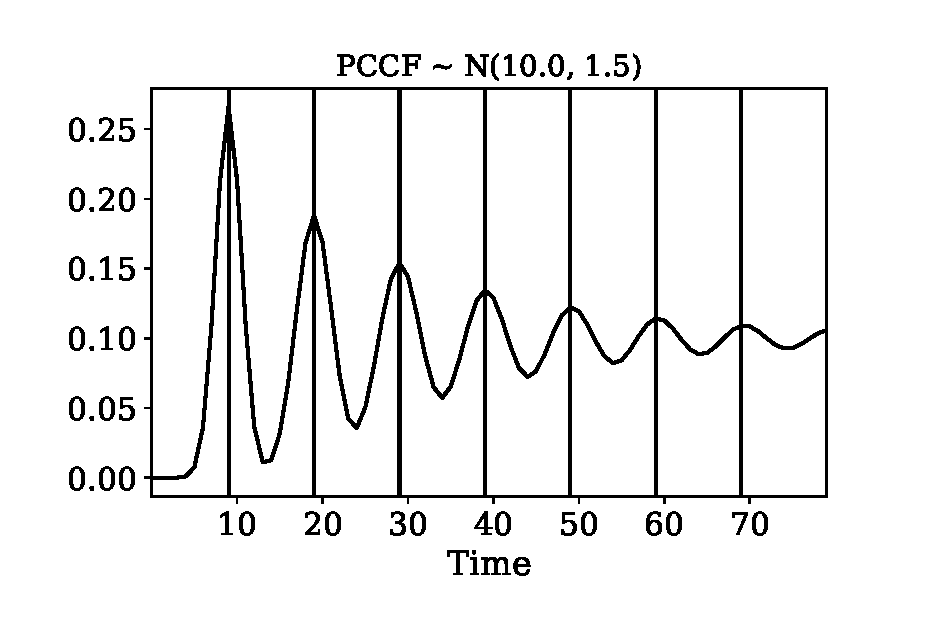
\includegraphics[scale=0.5]{img/pccf_example.eps}
%	\caption{
%		Gaussian PCCF.
%		The oscillating curve depicts probability estimation for the changepoint to occur at corresponding time moment.
%		Peaks are located at time moments $(\mu, 2 \mu, 3\mu, \dots)$.
%	}
%	\label{fig:pccf_example}
%\end{figure}
% Since Pccf decreases its values while oscillating and converging to the constant value over time we effectively choose first $k$ peaks of Pccf by applying threshold.
%By observing how fast Pccf converges to the constant level we can select $k$ based on visual inspection of Pccf behavior.
%Then we would need to select how many change points we need to predict
%After that ROI intervals can be allocated around Pccf's local extremums
\begin{figure}[!htb]
	\centering
	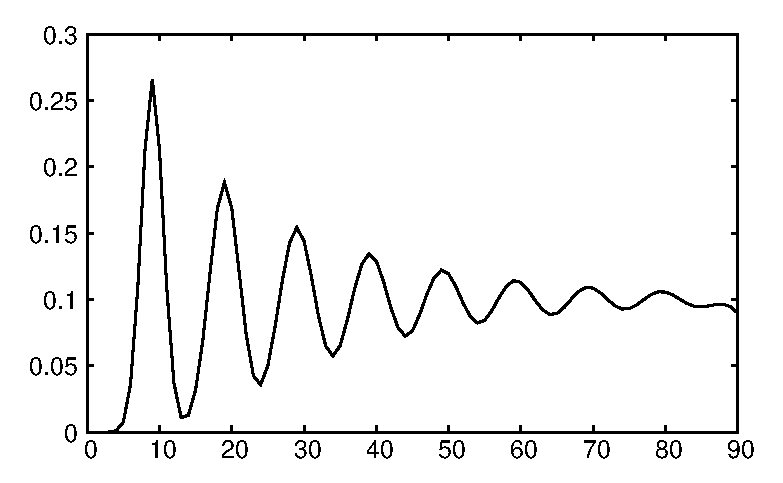
\includegraphics[width=0.7\textwidth]{images/example_pccf.eps}
	\caption{Pccf example}\label{fig:pccf_example}
\end{figure}



\section{Integration with Bayesian detector}
\section{Integration with CuSum}

\chapter{Article: CFB}

Article: Quantile Index for Gradual and Abrupt Change Detection from CFB Boiler Sensor Data in Online Settings.

\begin{abstract}
In this paper we consider the problem of online detection of gradual and abrupt changes in sensor data having high levels of noise and outliers.
We propose a simple heuristic method based on the Quantile Index (QI) and study how robust this method is for detecting both gradual and abrupt changes with such data.
We evaluate the performance of our method on the artificially generated and real datasets that represent different operational settings of a pilot circulating fluidized bed (CFB) reactor and CFB cold model. 
Our experiments suggest that QI can be used for designing very simple yet effective methods for gradual change detection in the noisy sensor data. It can be also used for detecting abrupt changes in the data unless they occur too often one after another.
\end{abstract}

\section{INTRODUCTION}
Sensor data and their analysis are used to monitor and control various types of processes in the systems.
Detecting changes in the time series signal gathered from the sensor is vital for many applications.
It is important to monitor an industrial process online in order to prevent undesirable process conditions.
For instance in the circulating fluidized bed (CFB) boilers particle size distribution is constantly changing.
Defluidization and insufficient heat transfer may cause an agglomeration of the bed particles.
This kind of events may lead to the shut down of the plant.

It is difficult to design a universal change detection method that would handle well different kinds of data and different kind of changes.
In practice, when designing a change detection algorithm, we need to use \emph{prior information} about the data and the anticipated changes if such information is available~\cite{I.V.Nikiforov}.

The term change point stands for a phenomenon when statistical properties of a data stream change over time.
Many approaches for statistical change (point) detection have been proposed in the literature, e.g.~\cite{Aggarwal05,Dasu06}. Some of them focused or suit particularly well on change detection in time series data, e.g.~\cite{journals/tkde/TakeuchiY06,cusum,BifetG07}.
Most of the proposed approaches rely on statistical change detection based on the monitoring of the changes in the data itself or in the outputs of the models learnt on that data. Most of the approaches are not parameter free and rely on certain assumptions about data, the expected change, and what is known about the possible values of the parameters before and after change~\cite{I.V.Nikiforov}.

In monitoring the operation cycles of the CFB boilers, we may deal with processes where we do not have any prior information, i.e.\ the online detection of change points in the sensor data is often complicated by the fact that data is noisy and may have an unknown dynamics.
In such cases thresholding heuristics often appear to be rather effective for an (abrupt) change detection with noisy data~\cite{ZliobaiteBP09}. 

In this paper, we propose Quantile Index (QI) -- a simple heuristic method based on quantile statistic aiming to handle at the first place the gradual changes in the noisy sensor data.
We focus on two basic cases: change (increase) in the mean and change (increase) in the variance of a noisy signal.

The rest of the paper is organized as follows.
In Section~\ref{sec:problem} we discuss the problem of online change detection in two different tasks -- pressure fluctuation and fuel mass flow estimation from the noisy sensor data.
In Section~\ref{sec:ourapproach} we first consider density ratio estimation and control charts as the traditional statistical change detection approaches and then present our QI method.
The results of our experimental study with the artificially generated and real data collected from the CFB test devices ~\cite{Tourunen,Gulden} are discussed in Section~\ref{sec:experiments}.
We demonstrate that QI is a promising heuristic for designing very simple and intuitive methods for change detection in a noisy sensor data.
Section~\ref{sec:conclusion} concludes.

\section{PROBLEM DESCRIPTION}
\label{sec:problem}

From combustion point of view the main challenges for the existing boilers are caused by a wider fuel selection, increasing share of low quality and bio fuels, and co-combustion. In steady operation, combustion is affected by the disturbances in the feed-rate of the fuel and by the incomplete mixing of the fuel in the bed, which may cause changes in the burning rate, oxygen level and increase CO emissions. This is especially important, when considering the new biomass based fuels, which have increasingly been used to replace coal.
These new solid biofuels may cause instabilities in the feeding. 
Biomass fuels have much higher reactivity compared to coals and the knowledge of the factors affecting the combustion dynamics is important for optimum control. The knowledge of the dynamics of combustion is also important for optimizing load changes~\cite{Saastamoinen04}. Data-mining approaches can be used to develop better understanding of the underlying processes in CFB boiler, or learn a model for optimizing its efficiency~\cite{PechenizkiyEtAl06}.

An inherent feature of the sensor signal from multiphase turbulent hydrodynamic flow in CFB boiler is that we often do not know
even approximately the value of the parameter of interest before and after change.
Also statistical properties of the signal are very vague in the sense that we cannot determine a distribution
from which data samples are being drawn.
This is due to the rapid changes on the combustion process dynamics.
Therefore, designing methods for online monitoring of the system parameters and detecting changes in them is not so straightforward.

We consider two different practical problems where online change detection is important; the problem of rapid particle size distribution (PSD) change detection and the problem of gradual change detection in online mass flow estimation in CFB boilers.

%\subsection{Particle Size Distribution change}
\subsection{Pressure fluctuation signal}

In the CFB technology crushed fuel and limestone are injected into the furnace.
The particles are suspended in a stream of upwardly flowing air which enters the bottom of the furnace through air distribution nozzles.
During the combustion process the fine particles are moved out of the furnace with a gas.
The particles are then collected by the solids separators and circulated back into the furnace~\cite{Kavidass}. 

Particle size distribution (PSD) changes over time. 
Uncontrolled change of PSD can cause undesirable process conditions, which may come out as problems with fluidization.
Partial defluidization may lead to bed material agglomeration and problems with bed removal.
These undesirable events affect combustion process and overall efficiency. Therefore change of PSD should be observed at the early stage.
Our goal is to introduce a change detection method for that.

In the laboratory experiment CFB cold model~\cite{Gulden} was equipped with pressure measurement. Pressure transducer was covered with metal mesh to prevent bed material contact.
During steady fluidization of the laboratory experiment at some moment of time particles with another average size were added to the bed material.
This addition of particles made step change to PSD and total bed mass of system.
It caused abrupt change in the measured signal as it can be seen in Figure~\ref{fig:psd_change}.
Further mixing of particles is depicted by gradual change in the amplitude of pressure.
It should be noted that since pressure fluctuation change was caused by adding particles with another size distribution this event was accompanied by increasing of total bed mass. That means that we can detect rapid change at increase of bed material and PSD, but we cannot be sure which one of these changes are dominant at measurement.

\subsection{Mass Flow Signal}

Fuel can be fed into the reactor through the feeding lines. There is a fuel screw feeder in each line at the bottom of the silo and a mixer, which prevents arching of the fuel in the silo.
The fuel silos are mounted on top of the scales. The scales measure weight over time, which can be presented as mass flow rate of the solid fuel.
The signal is fluctuating with constant screw feeder rotational speed. It depends on the quality of the fuel, e.g.\ moisture content and particle size.
The fuel inside the container is mixed using a mixing screw. Particles might jam in between the screw rotor and the stator causing a peak in the mass signal.
Fuel addition causes a step change in the mass signal. Figure~\ref{fig:OMF} illustrates the process and the signal.

During the burning stage the mass of fuel inside the container decreases (reflected by a decreasing amount of fuel in the data signal). As new fuel is added to the container (the burning process continues),
the fuel feeding stage starts that is reflected by a rapid mass increase~\cite{ZliobaiteBP09}.
The automatically available mass signal is a noisy estimate of fuel mass at each operation time point. The mass of the fuel inside the container is measured by a scale, with 1 Hz sample rate.

\begin{figure}[htb!]
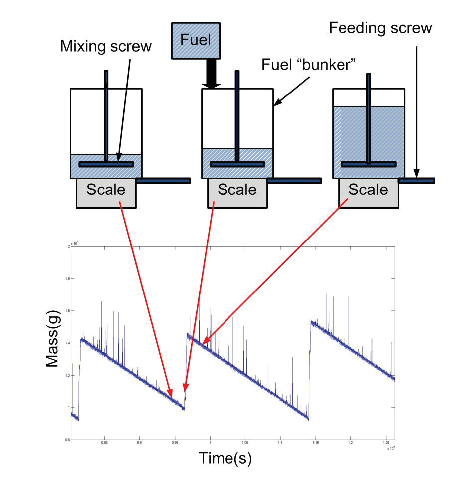
\includegraphics[width=0.45\textwidth]{pics/cfb_paper/OMF/MassFlowScheme}
\caption{The origin of the input signal ~\cite{ZliobaiteBP09}.}\label{fig:OMF}
\end{figure}

In the previous work~\cite{ZliobaiteBP09,BakkerSensorsKDD09,DBLP:conf/incdm/IvannikovPBLJKA09} outliers were removed,
burning and feeding stages were detected and mass flow was estimated with a high accuracy. The main results were summarized in~\cite{PechenizkiySIGKDDExpl09}.
However, occasional gradual changes in the signal caused by increasing or decreasing frequency of the mixing screw have not been addressed.
This is the problem that we focus on for this case.

\section{CHANGE DETECTION METHODS}
\label{sec:ourapproach}

There are many methods applicable to the problems we consider. We discuss here the density-ratio estimation and control charts which are fundamental for our domain and then present our Quantile Index (QI) approach.

\subsection{Density-Ratio Estimation}
The basic concept underlying the statistical change detection algorithms is the
logarithm of the likelihood ratio, defined by 
\begin{equation} \label{eq:lr1}
s(y) = ln \frac{p_{\theta_{1}}(y)}{p_{\theta_{2}}(y)}.
\end{equation}
% \subsection{Likelihood Ratio}
The likelihood of a sample is the probability of obtaining that particular sample,
given the chosen probability distribution model. This expression contains the unknown model parameters.
The values of these parameters that maximize the sample likelihood are known as the
Maximum Likelihood Estimates. 
A change in the parameter $\theta$ in (\ref{eq:lr1}) is reflected as a change in the
sign of the mean value of the log-likelihood ratio \cite{I.V.Nikiforov}.

But this approach is affordable in case if at least the parameter $\theta_{0}$ before the change is known.
In this case hypothesis testing between two hypotheses $H_{0}: \theta = \theta_{0}, H_{1}: \theta = \theta_{1}$
should be performed in an on-line manner by means of the decision function:
\begin{equation}\label{eq:lr2}
S_{j}^{k} = \sum_{i=j}^{k}  ln \frac{p_{\theta_{1}}(y_{i})}{p_{\theta_{2}}(y_{i})}.
\end{equation}
This is the underlying concept for control charts that we consider next.

\subsection{Shewhart control charts}

Statistical properties of the data can be marked on the graph by drawing an Upper/Lower Control Limits (UCL and LCL) for the selected feature $\theta$.
Control limits are two lines which indicate the state of the `in control' process.
It means that data points lie within those limits with a high predefined probability.
Strictly speaking we cannot use the term probability because we do not know a statistical distribution of the data.
But we can use a fraction of out-of-control points as an indicator of the state.
There is a probability that some points will fall outside the limits even if no actual change of feature $\theta$ has happened. 
The process can be described by the following three values:
\[ UCL = \mu_{w} + k\sigma_{w},\] \[Center Line = \mu_{w},\] \[  LCL = \mu_{w} - k\sigma_{w}. \]
The main object of interest is a set of rules defining when to update control limits.

The $CenterLine$ of the process and \textbf{$\sigma$} are unknown in general.
We just can estimate them from the set of sampled examples given some statistical assumptions. 
The standard deviation of the sample 
\[s = \sqrt{\frac{\sum_{k=1}^n (x_{i} - \overline{x})^2}{n-1}} \]
is just an estimator of the unknown standard deviation $\sigma$ of the data from which it is being sampled.
If the underlying distribution is known, e.g.\ normal, the corresponding parameters can be easily estimated~\cite{Nist}.

In manufacturing processes an action should be taken even if one point falls outside limits.
Due to specificity of our data we can determine a priori a threshold of the fraction of points which fall outside limits.
It changes over time and we have to deal with a streaming data which we have to treat on-line.
By monitoring the amount of points that fall outside control limits we can decide about the change and model update to be performed.

To keep the discussion compact we do not consider CUSUM control charts~\cite{cusum}.

\subsection{Quantile Index Method}
If we apply control charts we need to know the value of a statistical parameter, which changes over time, before the change.
Quantile Index (QI) is even a simpler approach and effectively is parameter free. 

Quantiles are points taken at regular intervals from the empirical cumulative distribution function that mark the boundaries between the consecutive subsets
(Figure~\ref{fig:PDD_quantile}).

\begin{figure}[htb!]
\centering
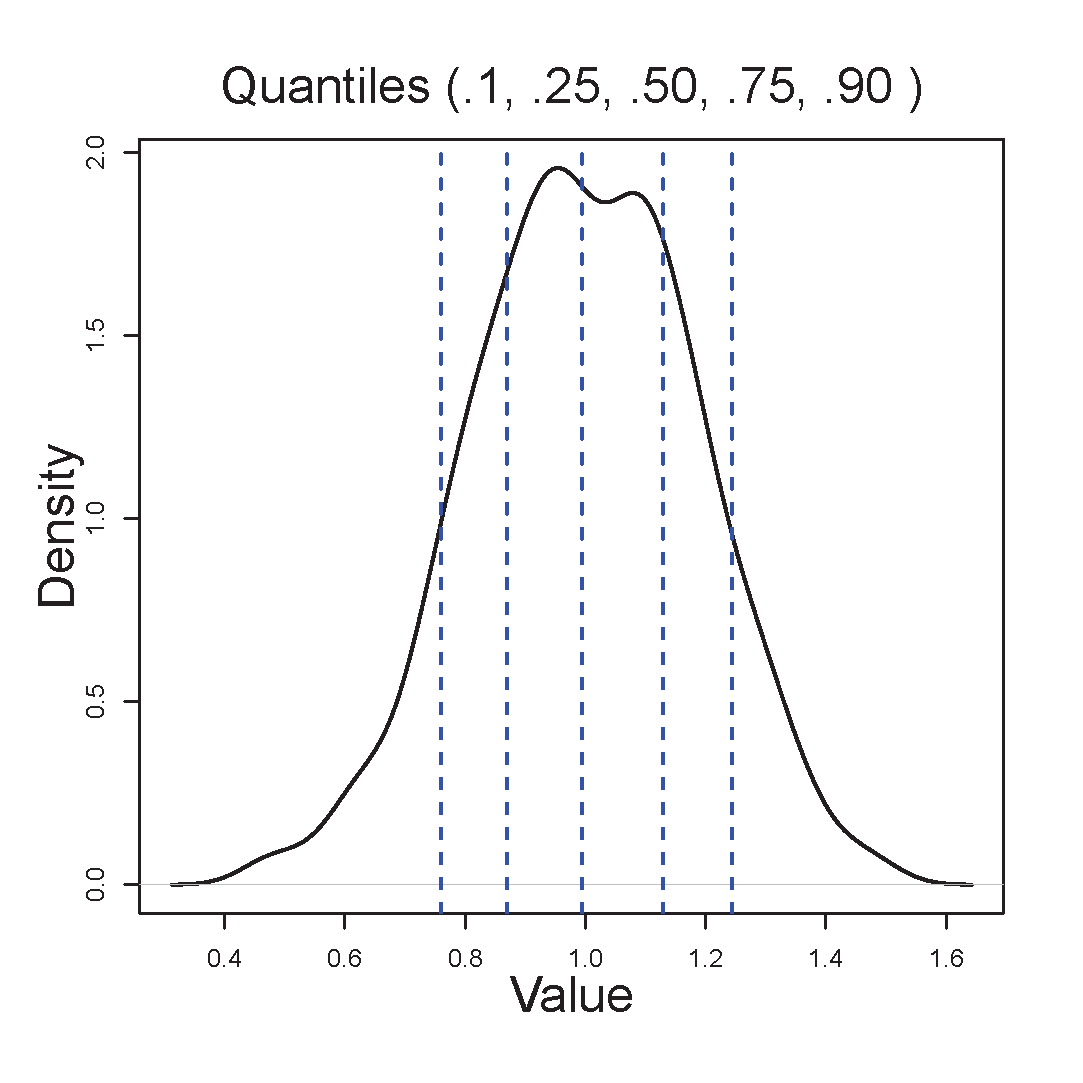
\includegraphics[width=0.4\textwidth]{pics/cfb_paper/QuantileDef}
\caption{The probability density distribution illustrating quantile values: $10\%$ of all points have values less than 0.76 (the first dashed line),
$15\%$ of all points lie between the first and the second dashed lines (because there are quantiles with probabilities $10\%$ and $25\%$), etc.}
\label{fig:PDD_quantile}
\end{figure}

We consider two basic cases: an increase in the mean and an increase in the variance of a signal. 
As an indicator of a state we keep track of the top boundary of the data points by moving quantiles with maximum probability. 
When a change has happened we observe a kind of step function. By selecting an appropriate width of a sliding window we make this track line insensitive to outliers; but it allows us to detect steady changes.
For this purpose we use two quantiles with probabilities $90\%$ and $100\%$.
The intuition is that after a change there is no intersection between the data points falling in between the current $90-100\%$ quantiles and between the same quantiles in the past. Therefore QI will demonstrate a sharp change even in the case of a gradual change in the signal.

The change detection method based on QI works as follows:
\textit{
At each moment of time we consider a range of data which is divided into two subsets corresponding to the Test Interval and the Reference Interval.
We compute the minimum Index of observations in the Reference window which values are in the range between quantiles of the measurements in a Test window} (Figure~\ref{fig:QI_scheme}).

\begin{figure}[htb!]
\centering{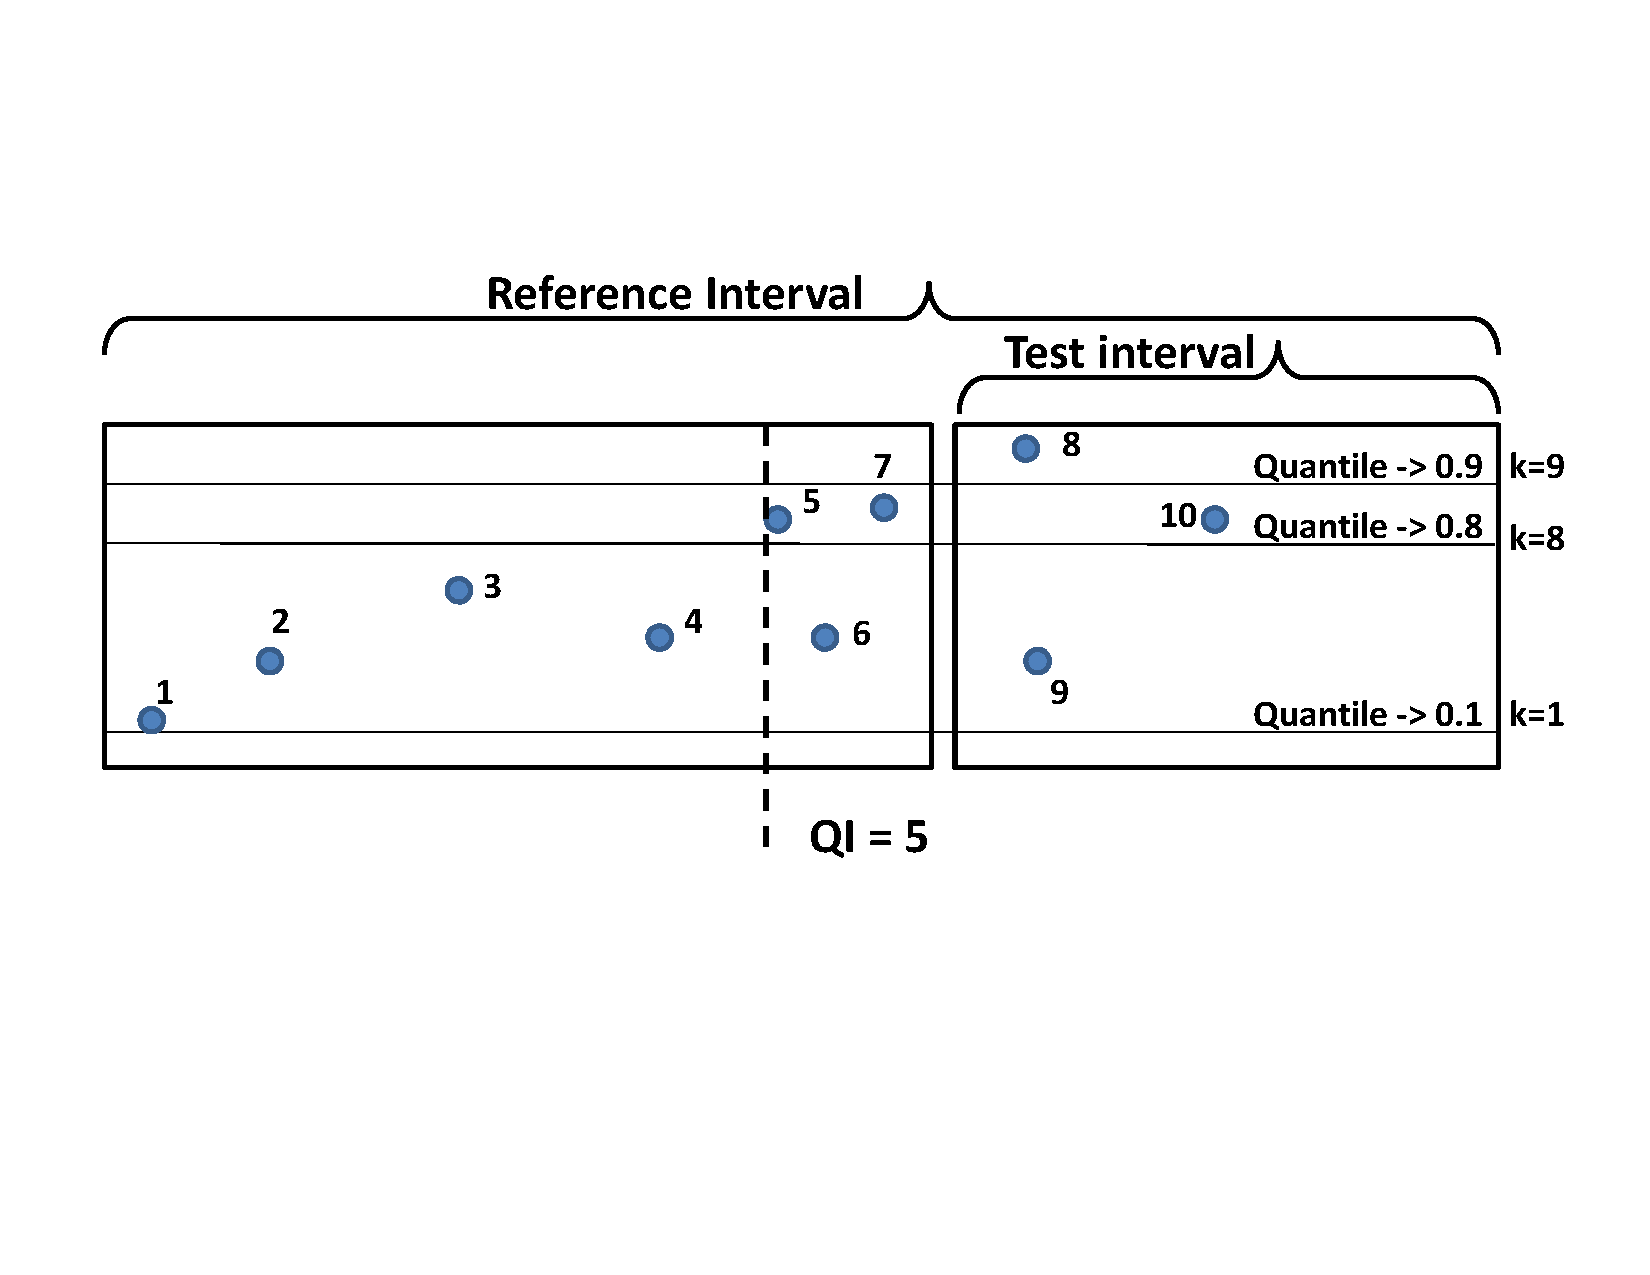
\includegraphics[width=0.45\textwidth]{pics/cfb_paper/QIdefinition}}\\
\caption{QI method illustration. %Beginning of the \emph{reference interval} should start from the last detected change or from the beginning of a signal if there has been no change detected so far.
QI depicts the position of a point with the smallest index which lies between quantile 0.9 limits
in the Test interval.}
\label{fig:QI_scheme}
\end{figure}

Thereby we determine a `similarity' between chunks of the data.
Quantiles are computed from the inverse of the empirical distribution function.
In other words, the $p$'th quantile of $X(0<p<1)$ is defined by:
\[
Q_{p}=F_{X}^{-1}(p).
\]
Given the probability $p$ and sorted data vector $x$, quantile estimation could be calculated as follows:
\[
Q(p) = (1-\gamma)x[j] + \gamma x[j+1],
\]
where $j=floor(np)$, $n$ is the sample size, $\gamma = 0$ if $p=0$, and $1$ otherwise \cite{Rref}.
There are two ways for calculating statistics on-line.
One approach is to calculate it over a sliding window at each moment of time. %(Short QI).
The second way is to calculate cumulative statistics from the beginning up to the current moment.
It is more robust but also more computationally expensive.
We compute QI for both cases by means of different sizes of a sliding window.
The pseudocode for computing cumulative QI for the current Reference and Test Intervals is presented below:
\begin{verbatim}
w - window width; 
i - data point sliding index;
Q - array to store quantiles;
k = 10 - index determining quantiles to be used;
QI - quantile index returned as an output;

Reference Interval <- data[1:i]
Test Interval <- data[(i-w+1):i]
# array of probabilities:
Probability  <- {0.1,...,0.9,1}
Q <- quantile(Test Interval, Probability)
QI <- which((Reference Interval >  Q(k-1)) and
            (Reference Interval <= Q(k)))
QI <- minimum(QI)
\end{verbatim}

Function \textit{which()} returns indexes of data points which satisfy condition in brackets. For the example in Figure~\ref{fig:QI_scheme}, \textit{which()} will return $\{5,7,10\}$ and consequently, $QI=5$.
These calculations should be performed for each time step over a sliding test interval.

\section{Experimental study}
\label{sec:experiments}
First, we show the behavior of QI on the artificial data. 
We show explicitly values of $90\%$ and $100\%$ moving quantile values by which QI is being determined and the sensibility of QI to perturbations in the signal which affect quantiles online estimation.
Then, we evaluate the performance of QI and other considered approaches on two real datasets.

\subsection{Artificial Data}
We compute QI values for generated data with known statistical properties in order to
demonstrate behavior of QI depending on the test interval width.
There are three blocks of samples from uniform distribution each length of 1000 with a range width equal to 1 (Figure~\ref{fig:figure3.0}).
Each block is shifted by the $step = 0.15$ relative to the previous one.
The artificial data is produced in a similar way as described in ~\cite{journals/tkde/TakeuchiY06,Kawahara_2009}.

\begin{figure}[htb!]
\centering{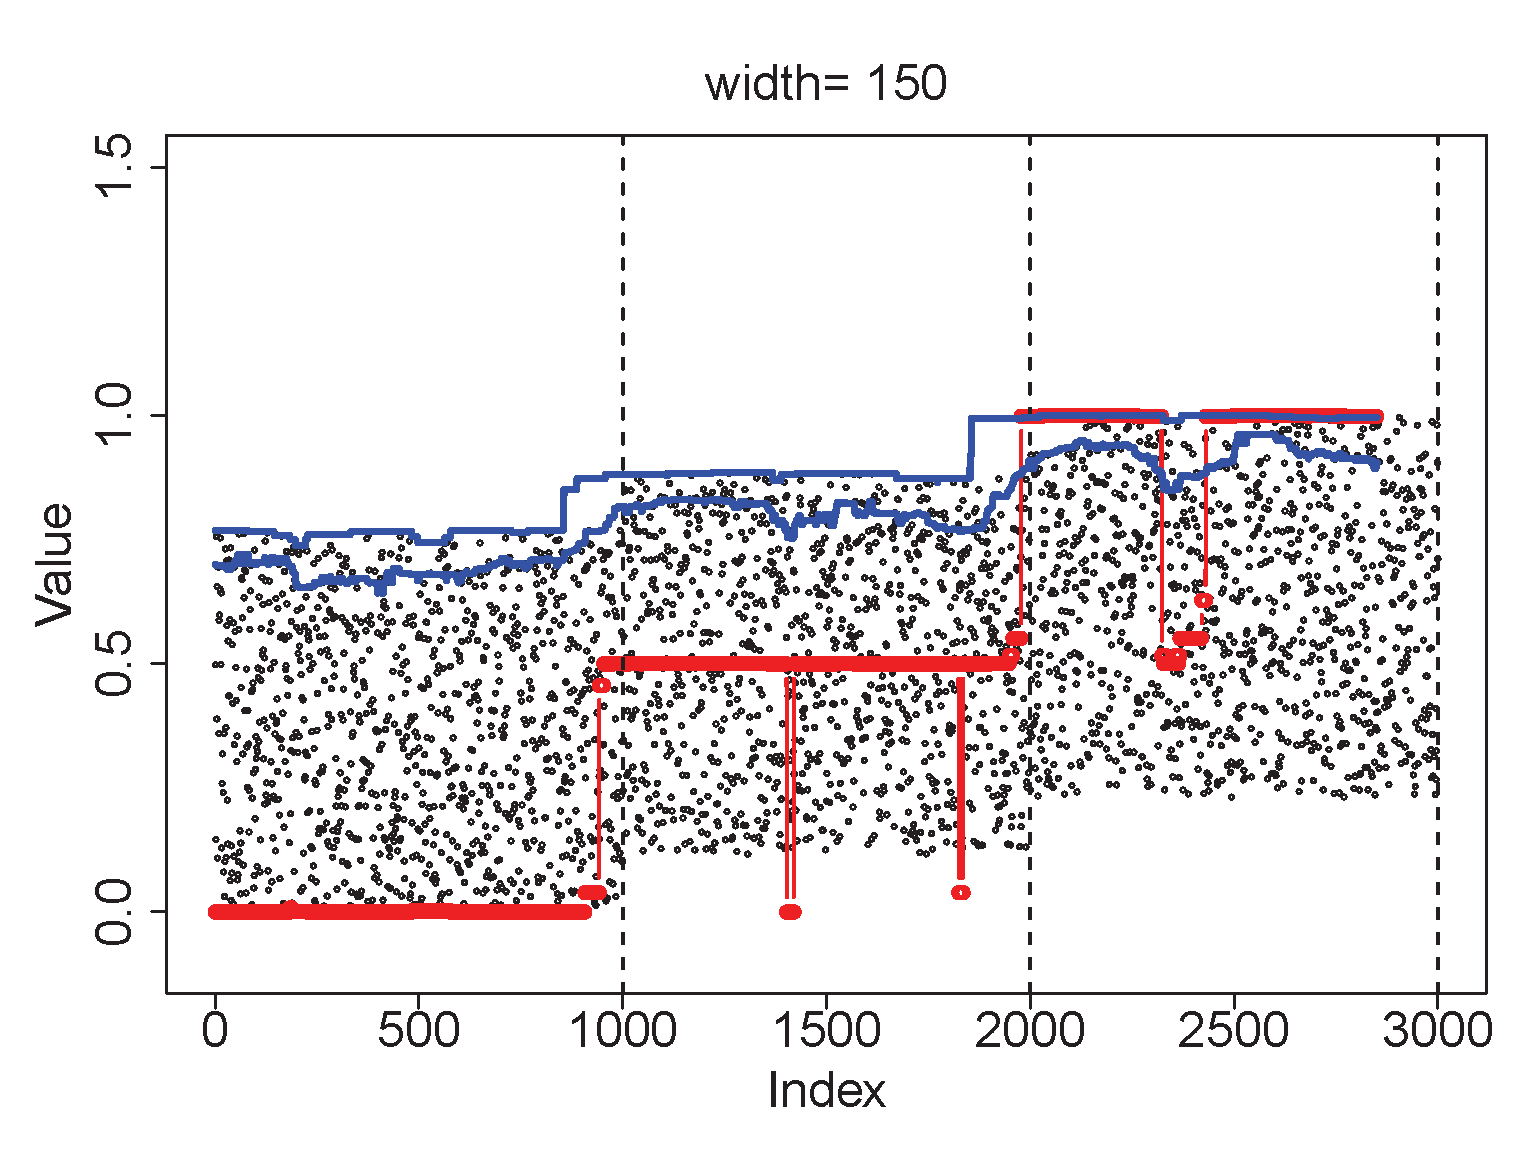
\includegraphics[width=0.45\textwidth]{pics/cfb_paper/DebugDataSet/DataPIC150}}\\
\centering{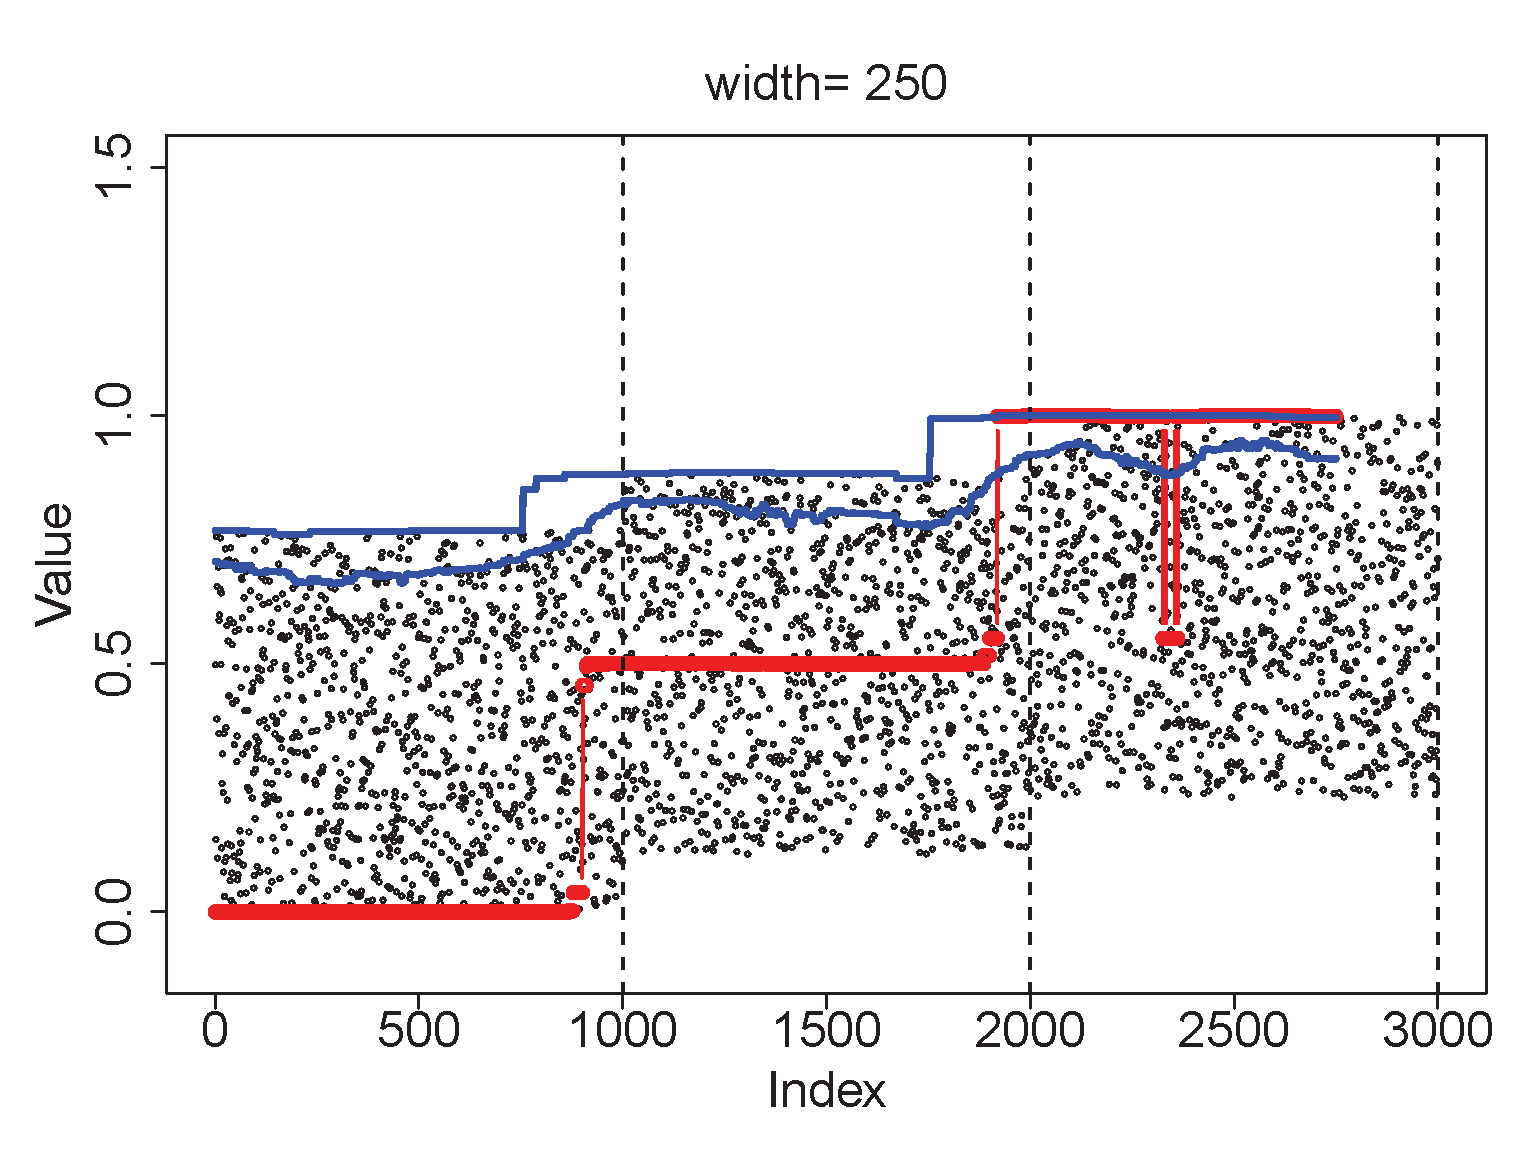
\includegraphics[width=0.45\textwidth]{pics/cfb_paper/DebugDataSet/DataPIC250}}
\caption{Behaviour of scaled QI values (red dots), quantiles values (blue dots) for uniformly distributed data (black dots).}
\label{fig:figure3.0}
\end{figure}

\begin{table}[htb!]
%\centering
\caption{Performance of QI on the artificial data. The bigger the test interval the more robust to quantiles values fluctuations QI is.}
\begin{tabular}{|l|l|l|l|l|l|l|}
\hline
	Test Interval width            & 50  & 70  & 90  & 120 & 130 & 150 \\ \hline
	False alarm rate & 19  & 10  & 8   & 6   & 6   & 5   \\ \hline
	Test Interval width			 & 170 & 190 & 210 & 230 & 250 &     \\ \hline
	False alarm rate & 4   & 3   & 2   & 1   & 1   &     \\
\hline
\end{tabular}
\label{Table1}
\end{table}

\subsection{Pressure fluctuation change}

The dataset comes from the controlled experiment in the laboratory settings. The sensor was measuring the dynamic gas pressure in the cold model CFB system.

The dataset consists of 3 800 001 data points (the sampling rate dt(s): 5000 Hz) corresponding to the duration of 12 minutes and 40 seconds.
%The measurements were taken with high frequency.
We consider down sampled signal for the computational and visualization convenience.
The sample frequency 20 Hz for pressure fluctuations can be considered as a lower limit.
But typically, a sample frequency in the order of 200-400 Hz is applied ~\cite{vanOmmen2011403}.

At a particular moment, particles with another average size were added inside a container.
It caused abrupt change in the signal (Figure~\ref{fig:psd_change}, $t=223$). Further mixing of particles is manifested by the gradual change in the amplitude of pressure. The signal is symmetrical because we use the first difference of the original signal.

\begin{figure}[htb!]
\centering{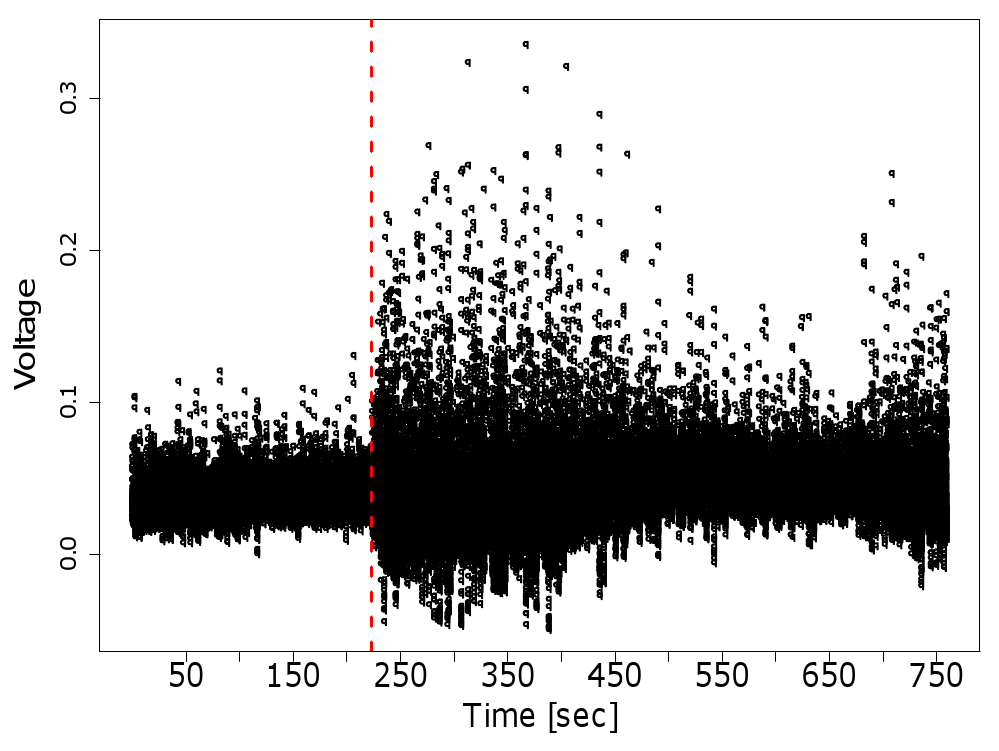
\includegraphics[width=0.45\textwidth]{pics/cfb_paper/PSD/PSDsampled}}
\caption{Adding of particles with another PSD.}\label{fig:psd_change}
\end{figure}

Figure~\ref{figure7} shows the Box-And-Whisker diagram, in which each box represents 5 values: the largest and smallest values, median, and the highest and lowest quartiles. From the diagram we can see more explicitly the gradual change near the 16th-17th data windows.

\begin{figure}[htb!]
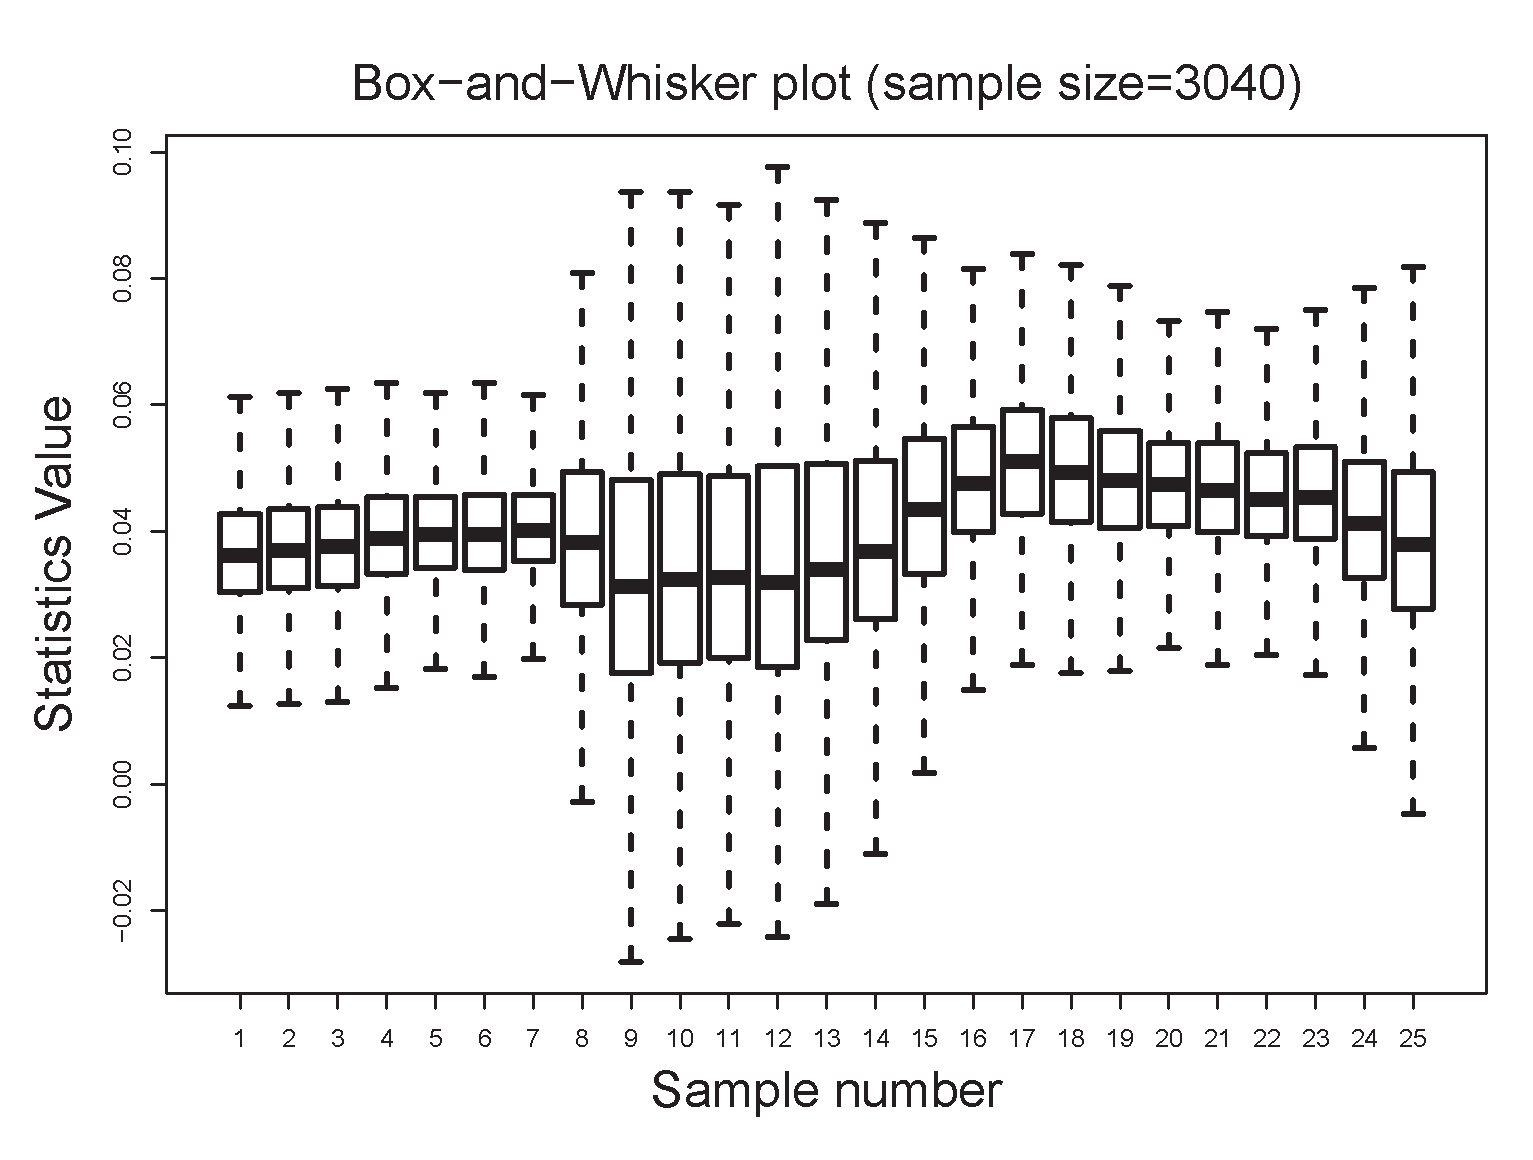
\includegraphics[width=0.45\textwidth]{pics/cfb_paper/PSD/PSDboxplot}
\caption{Box Plot for sampled signal. Signal was divided into groups of samples. Each box
on the graph represents 5 statistics for each group.}\label{figure7}
\end{figure}

Figure~\ref{figure8} shows the probability density estimations of the data before and after change. We can see that the averages are almost the same, but the standard deviation values are quite different.

\begin{figure}[htb!]
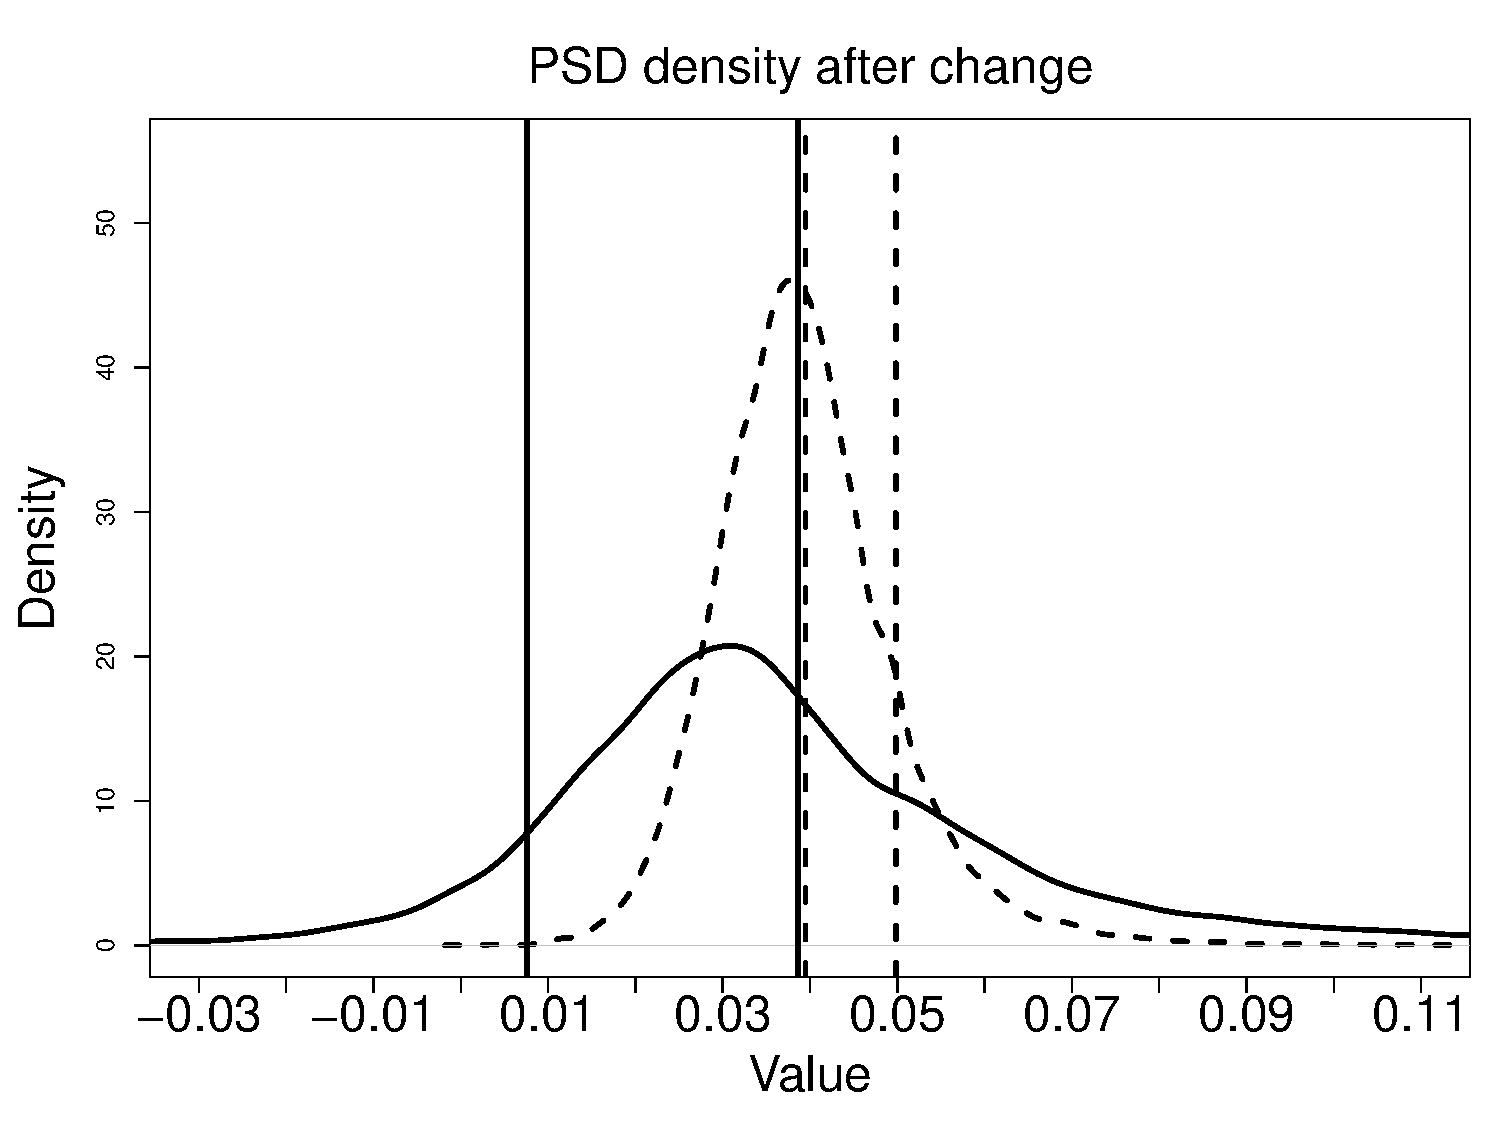
\includegraphics[width=0.45\textwidth]{pics/cfb_paper/PSD/PSDdensity}
\caption{Estimation of a probability density of a signal before and after change.}\label{figure8}
\end{figure}

From Figure~\ref{figure9} we can see that the most significant change happened in the standard deviation and the range of values:
$(Mean2 - Mean1)/Mean1 = 0.02$, $(Std2 - Std1)/Std1 = 1.99$. The first 250 seconds time range is considered as process in control, because we know that no particles have been added by this moment and some time after. Accordingly to the standard rules, the process in control points should fall within $3\sigma$ limits. 

\begin{figure}[htb!]
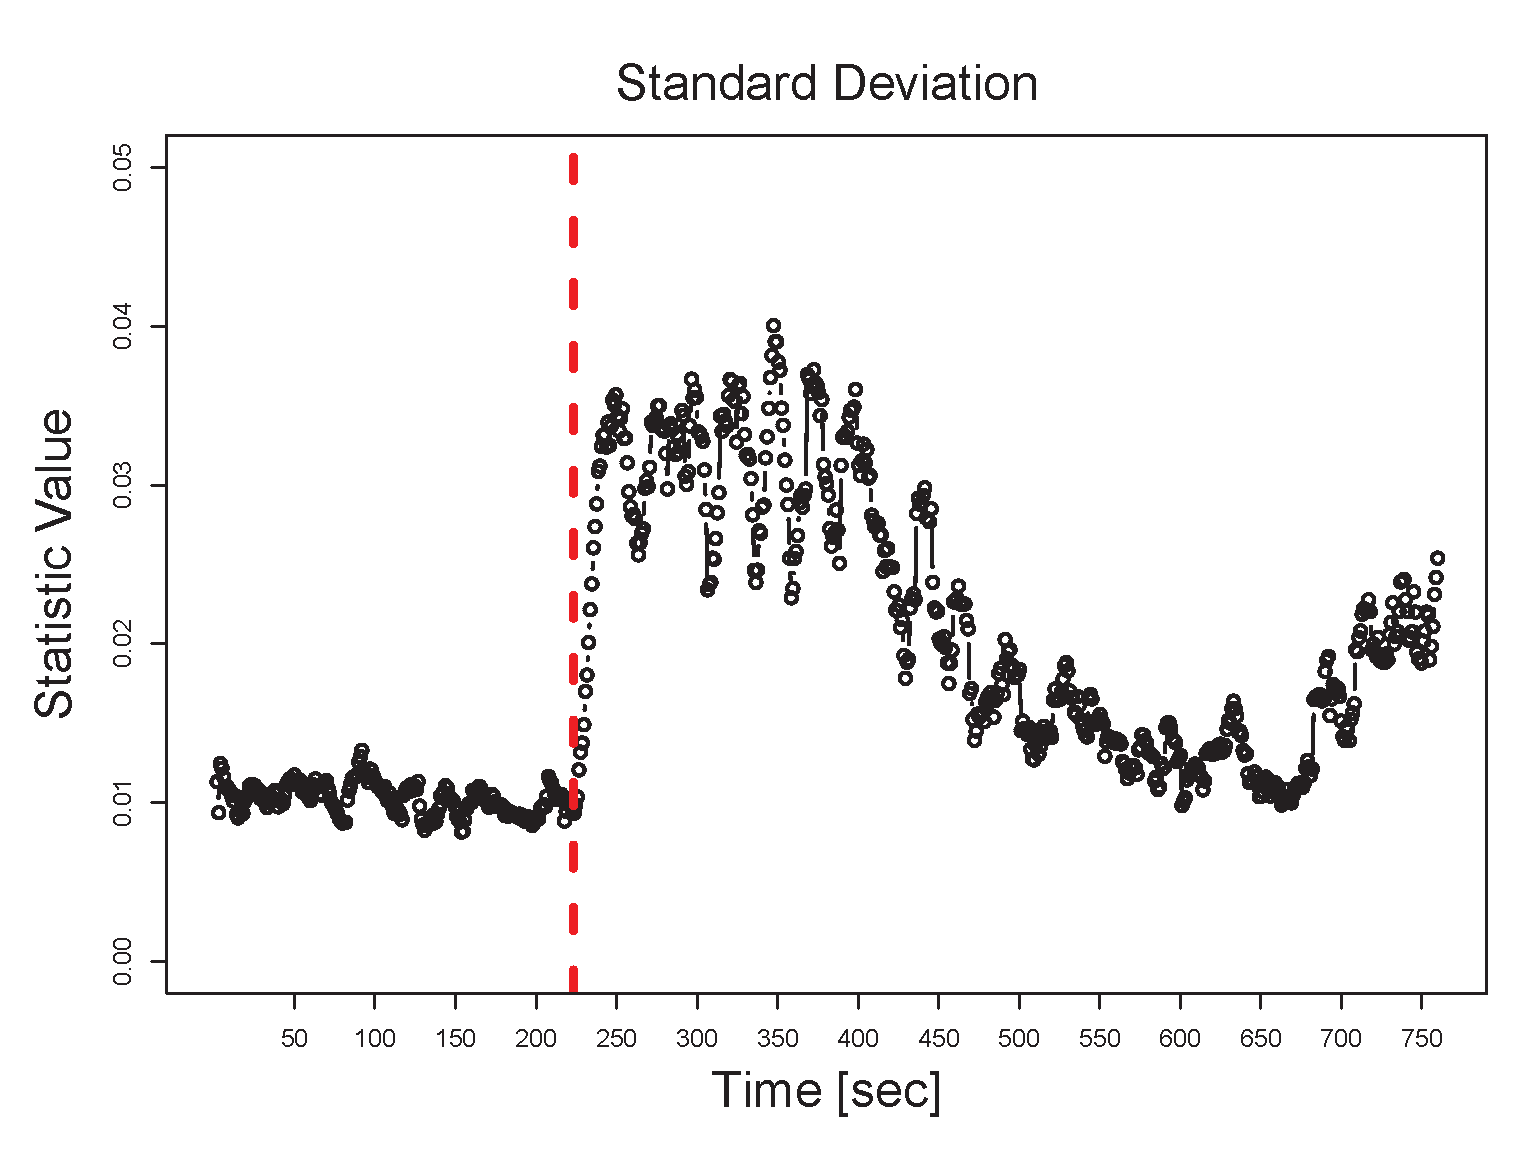
\includegraphics[width=0.45\textwidth]{pics/cfb_paper/PSD/PSDsd}
\caption{Moving standard deviation -- a promising feature to use for change detection.}\label{figure9}
\end{figure}

\paragraph{Change detection with Control charts for moving SD}
We consider the first difference of the moving standard deviation.
We define new control limits for a process each time when we have more than $10\%$ points beyond control limits and
when current control limits are greater more than 1.5 times than $3\sigma$ (Figure~\ref{figure10}).

\begin{figure}[htb!]
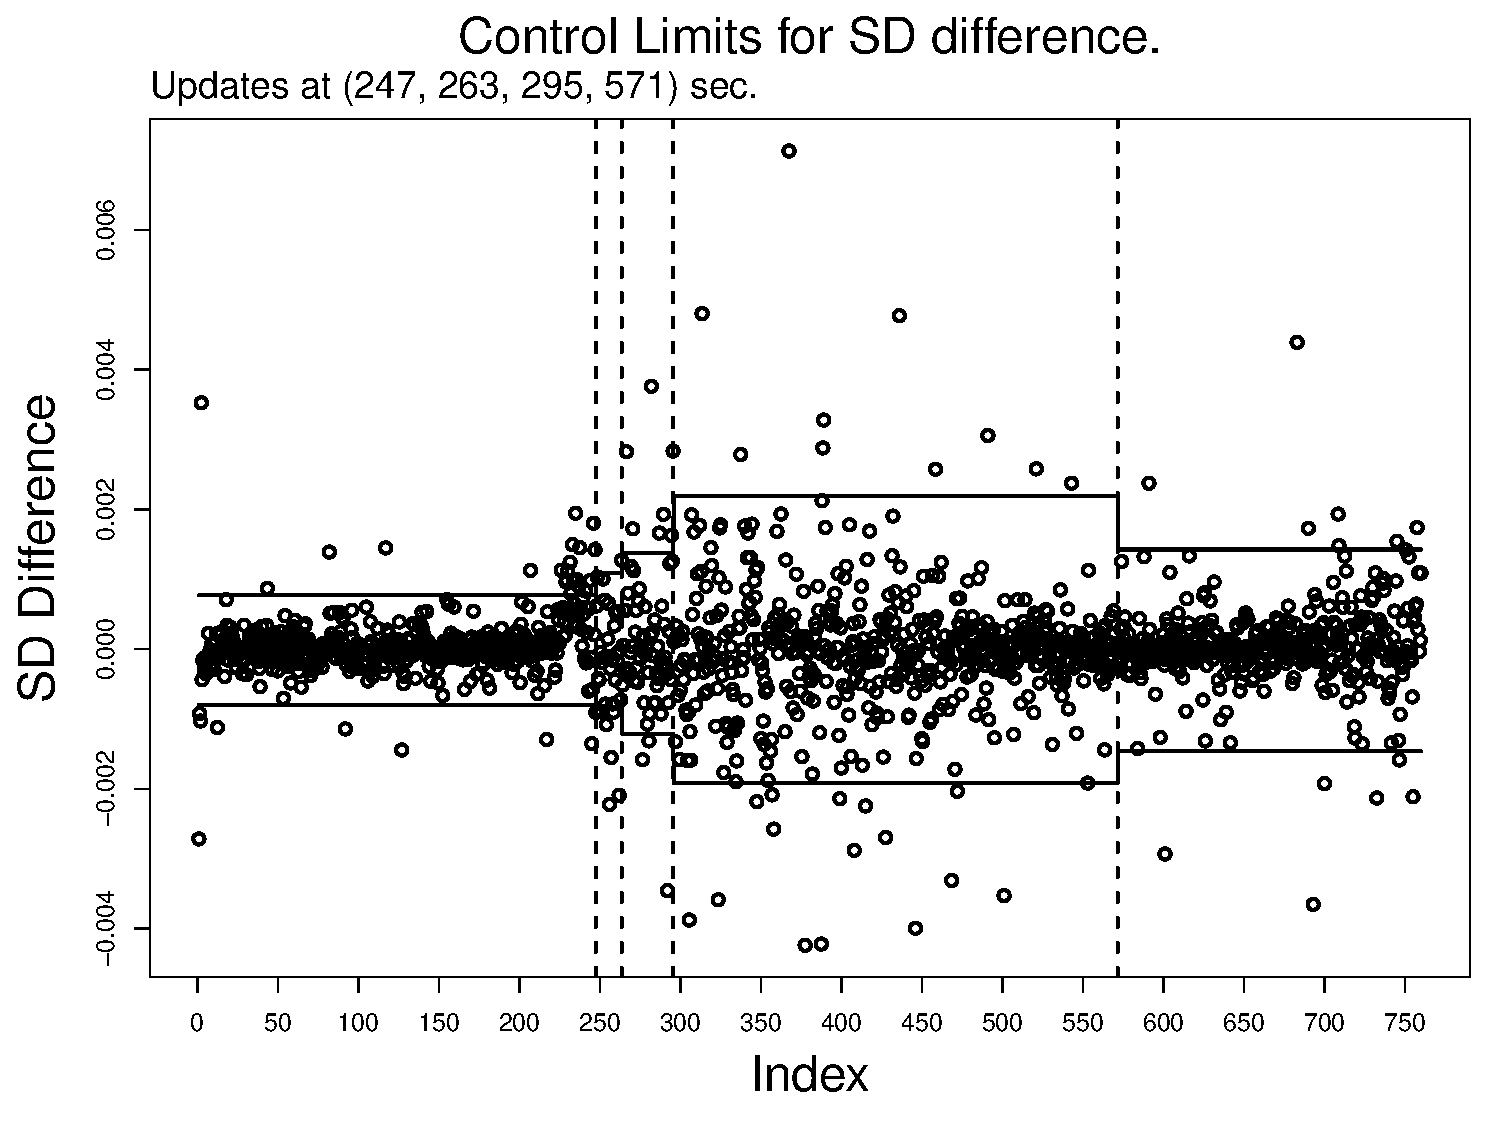
\includegraphics[width=0.45\textwidth]{pics/cfb_paper/PSD/PSDrunnqccSD}
\caption{Control charts for the first order difference of the moving standard deviation.
New control limits are updated each time when more than $10\%$ of points fall beyond limits.}\label{figure10}
\end{figure}

Updates were performed four times: $t=\{247, 263, 295, 571\}$. 
The latency of the detection is $(247-223)=24$ seconds.

\paragraph{Detection with Quantile Index}
%Let's apply QI for the same data.
We can use different features in order to apply control charts.
But which one is the most sensitive to the abrupt changes and for gradual changes?
QI is robust to outliers and noise presence; therefore we can apply it directly to the raw data.
We detect a change in case of significant increasing of QI values relatively to the previous QI.
The criterion we us is 
\begin{equation}\label{QIcriterion}
log \frac {QI[i]}{QI[i-1]} \geq threshold.
\end{equation}
%$log(QI[i]/QI[i-1]) >= threshold$.
Change points detected with QI are shown in Figure~\ref{figure12}. The latency of the detection for the known change at $t=248$ is $(248-223)=25$ seconds.

\begin{figure}[htb!]
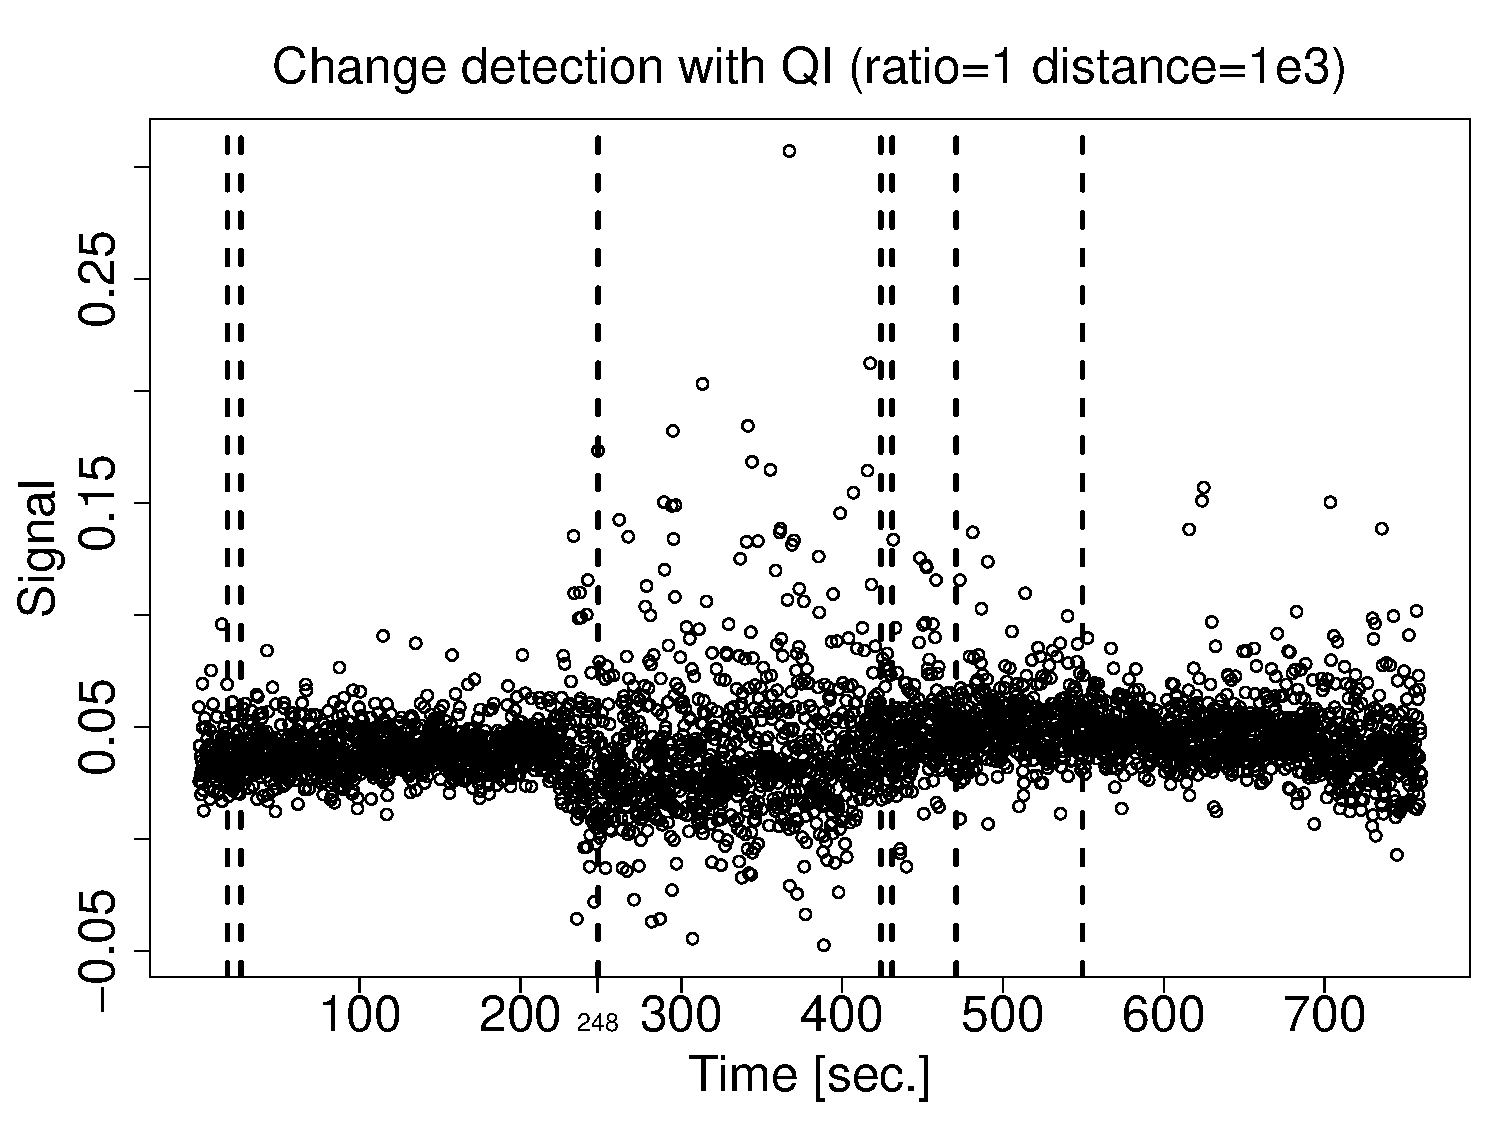
\includegraphics[width=0.45\textwidth]{pics/cfb_paper/PSD/PSDsteadyQI1}
\caption{Change detection with QI on raw data.}\label{figure12}
\end{figure}

\paragraph{Detection with Density Ratio Estimation}

Modifying eq.~\ref{eq:lr2} to our reference and test intervals we get
\begin{equation}\label{KDEformula}
S = \sum_{i=1}^{n_{te}}  ln \frac{p_{te}(Y_{te}(i))}{p_{rf}(Y_{te}(i))},
\end{equation}
where
\begin{equation}
w(Y)=\frac{p_{te}(Y_{te}(i))}{p_{rf}(Y_{te}(i))}
\end{equation}
is the density ratio.

Further we conclude
\begin{equation}
\begin{cases}
S \leq \mu \rightarrow \phantom{1} no \phantom{1} change \phantom{1} occurs, \\
otherwise  \rightarrow \phantom{1} a \phantom{1} change \phantom{1} occurs,
\end{cases}
\end{equation}
where $\mu >0$ is a predetermined threshold~\cite{Kawahara_2009}.

Figure~\ref{figure12.1} shows change detection results with the online non-parametric Kernel Density Ratio estimation (KDE) algorithm.
\begin{figure}[htb!]
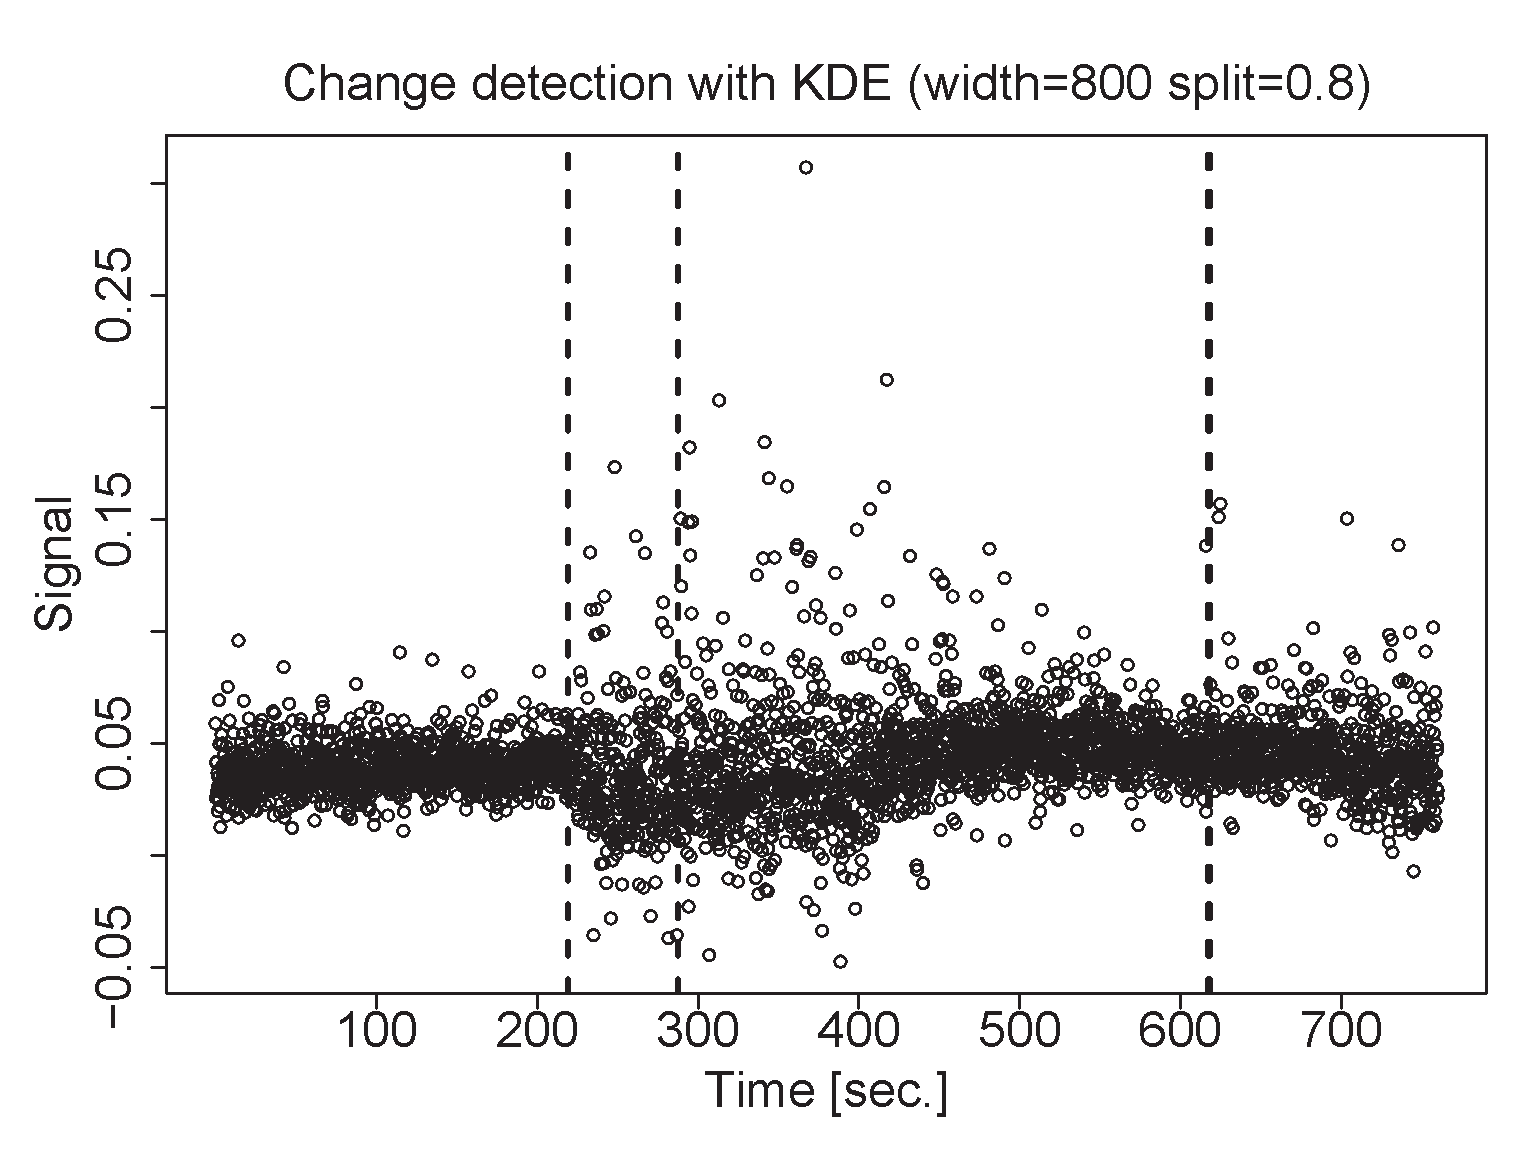
\includegraphics[width=0.45\textwidth]{pics/cfb_paper/PSD/PSDkde}
\caption{Change detection with KDE. Detected points: $t=\{219,274,614\}$.}
\label{figure12.1}
\end{figure}

\subsection{Mass Flow Signal}

The signal has the following properties. It reflects burning and feeding stages (both are abrupt changes).
The signal itself is noisy due to the disturbances of the physical system that vibrates and shakes from time to time when particles are jammed with the mixing screw.
Besides, there is a room for gradual change due to change in the mixing screw frequency.
Although the change in the signal is gradual, it was caused by abrupt change in the frequency -- see Figure~\ref{figure15} for the illustration.
We should notice that there are a lot of not only noise but outliers too that
makes change detection and especially gradual change detection rather challenging.
Figure~\ref{figure18} shows the both the abrupt and the gradual changes.

\begin{figure}[htb!]
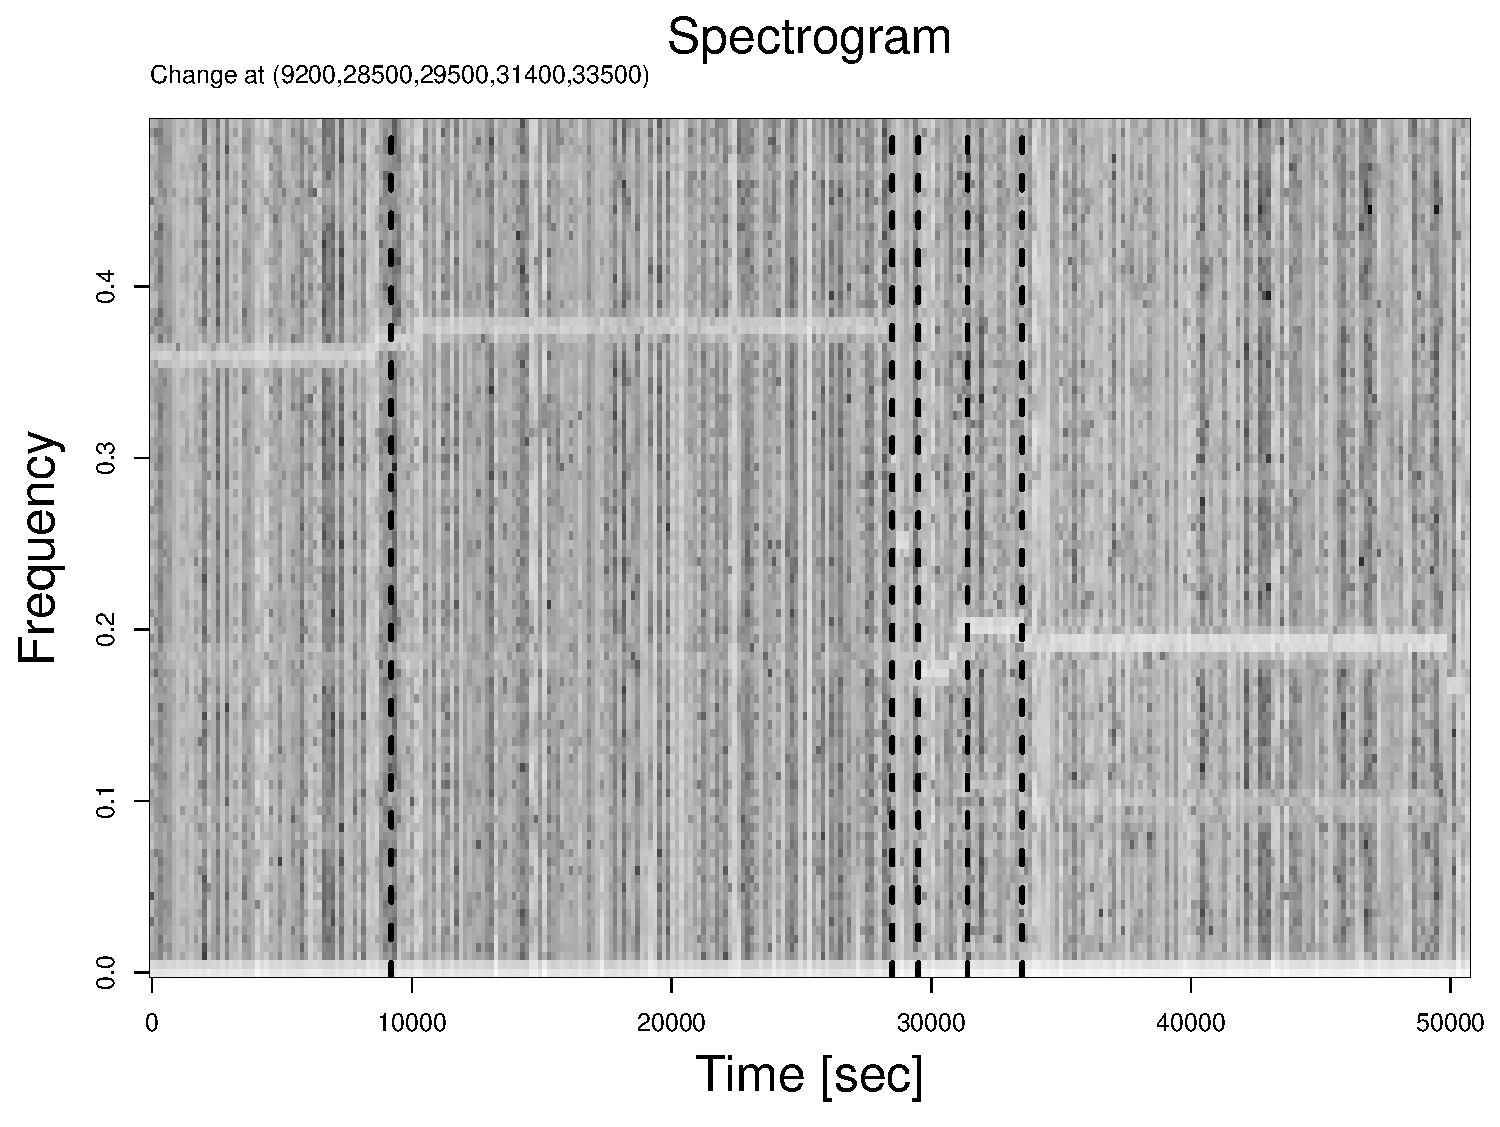
\includegraphics[width=0.45\textwidth]{pics/cfb_paper/OMF/OMFspg}
\caption{Spectrogram showing frequency changes.}\label{figure15}
\end{figure}

As a fuel mass estimation we use the sequence of points at the bottom of a signal, or, in other words, the lowest quantile at each moment of time (Figure~\ref{figure16}).

\begin{figure}[htb!]
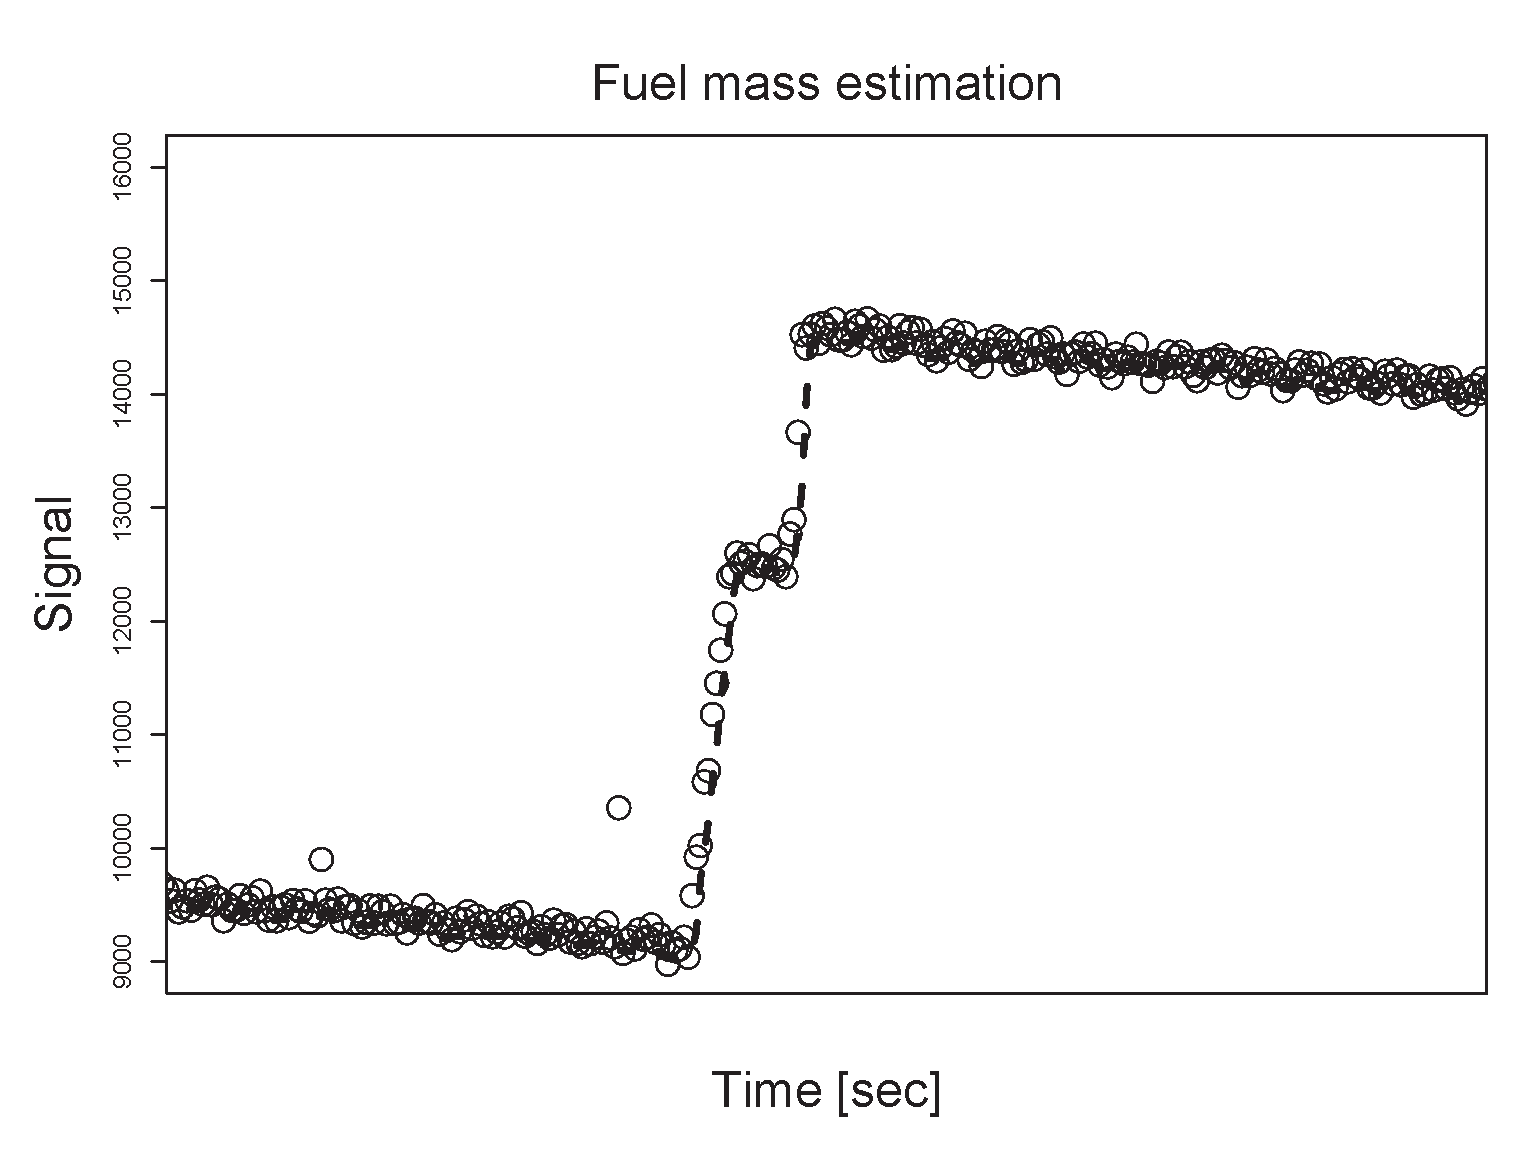
\includegraphics[width=0.45\textwidth]{pics/cfb_paper/OMF/OMFestim2}
\caption{Fuel mass estimation using $5\%$ quantile (dashed line) computed over the sliding window.}\label{figure16}
\end{figure}

\begin{figure}[htb!]
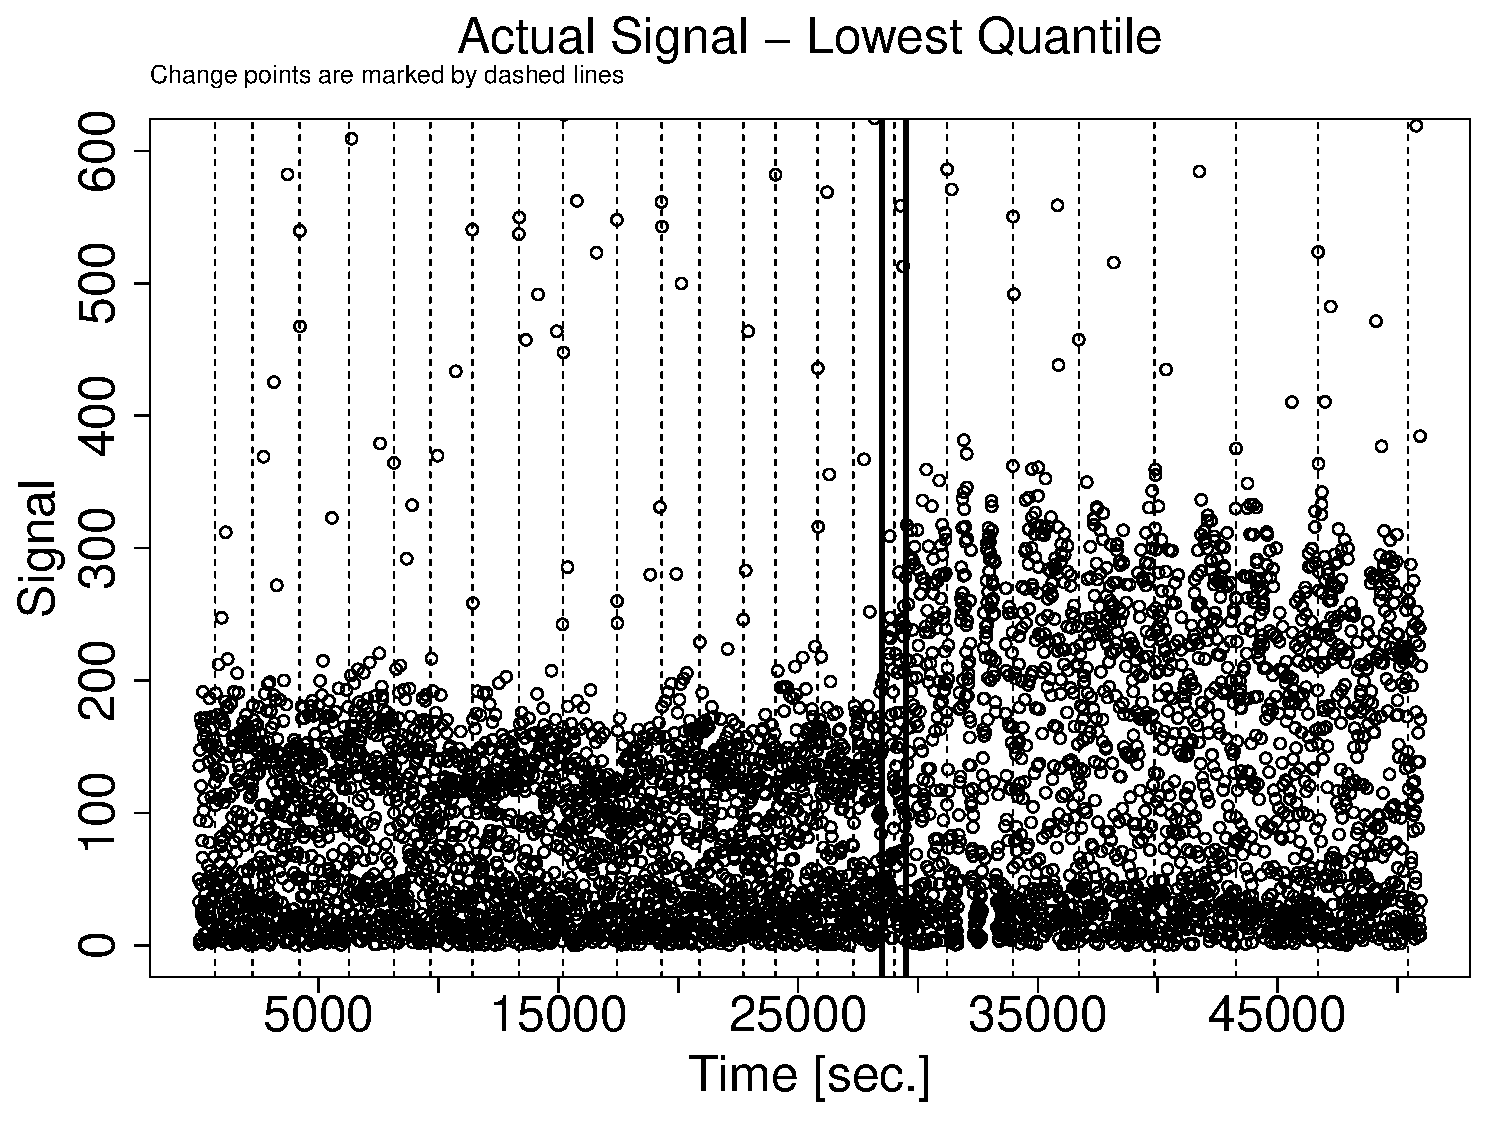
\includegraphics[width=0.45\textwidth]{pics/cfb_paper/OMF/OMFscalednoise}
\caption{Mass flow signal with marked change points, determined by visual inspection of the original signal and the spectrogram.
There are a lot of changes due to switching between burning and feeding stages (depicted by thin dashed lines) and
two changes due to the screw frequency change (two bold solid lines).}
\label{figure18}
\end{figure}

\paragraph{Change detection with QI}
The signal is highly noisy.
There is a mixture of a changes of different types (outliers, feeding-burning stages, gradual changes).
And it is not easy to find an appropriate statistic convenient to control the process.
For example, the moving average has a form which is shown in Figure~\ref{figure19}.
No part of such feature is `in-control' in the sense that in-control process is the process
when the data points fall between $3\sigma$ control limits.
The standard deviation is even more non-stationary (Figure~\ref{figure20}).

\begin{figure}[htb!]
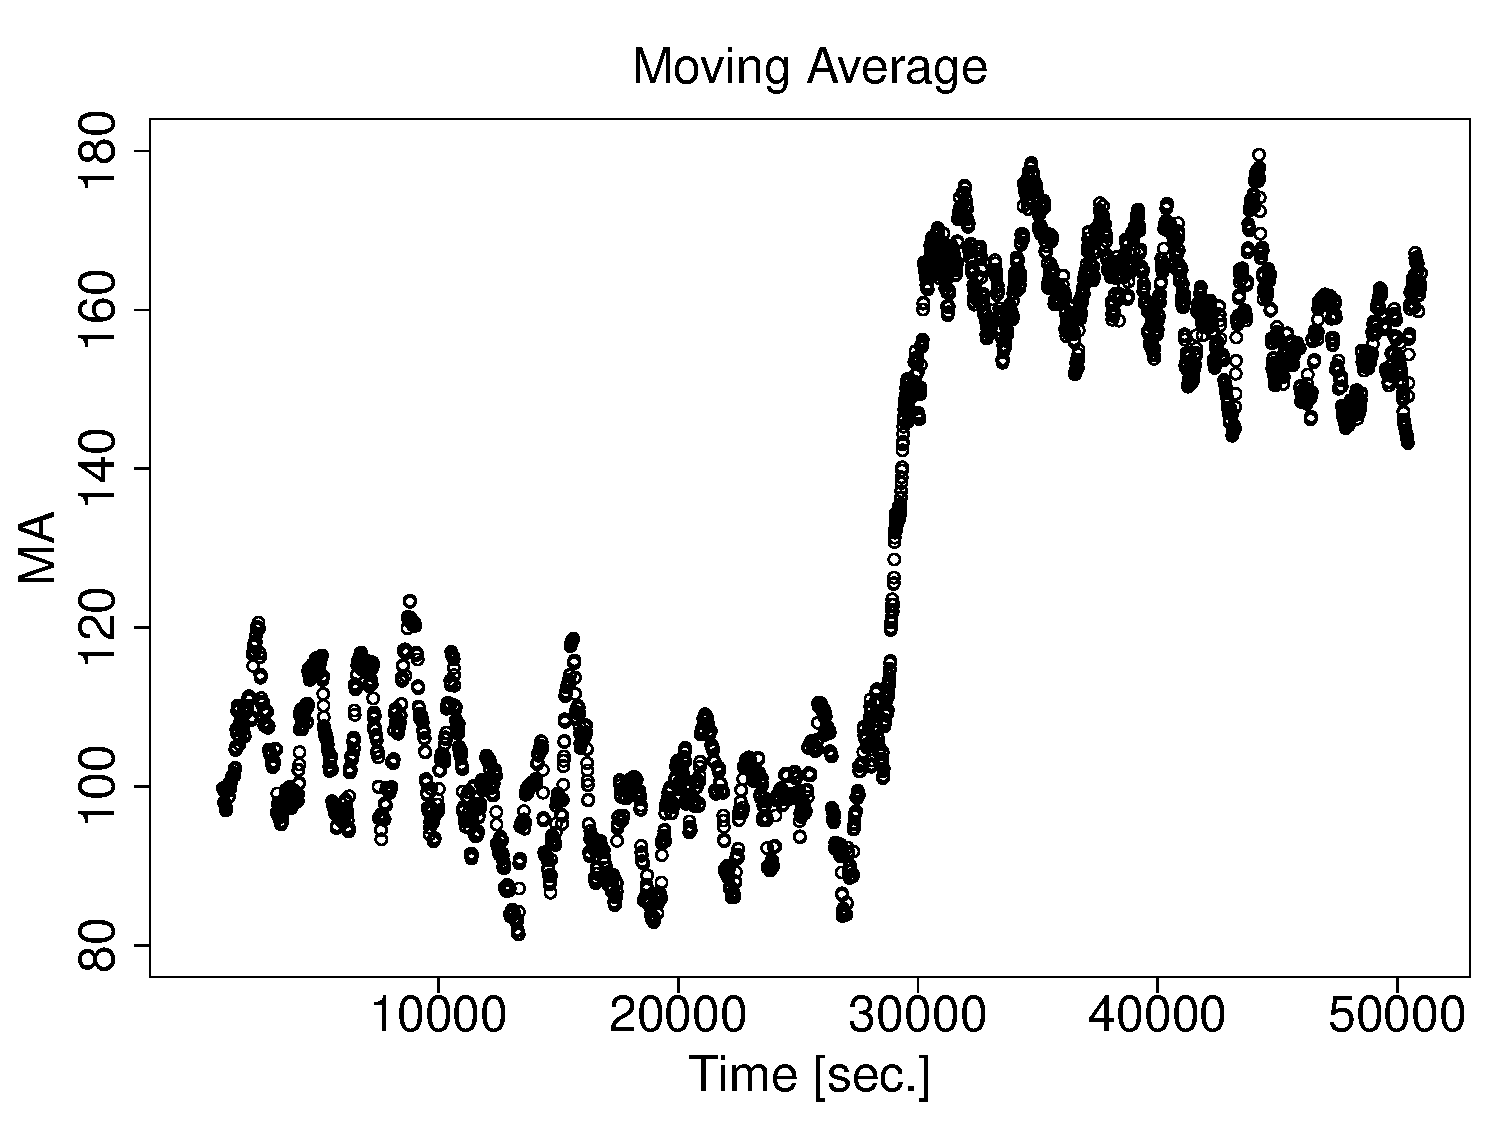
\includegraphics[width=0.45\textwidth]{pics/cfb_paper/OMF/OMFrma}
\caption{Moving average for the difference of the original signal and the fuel mass estimation.}\label{figure19}
\end{figure}
\begin{figure}[htb!]
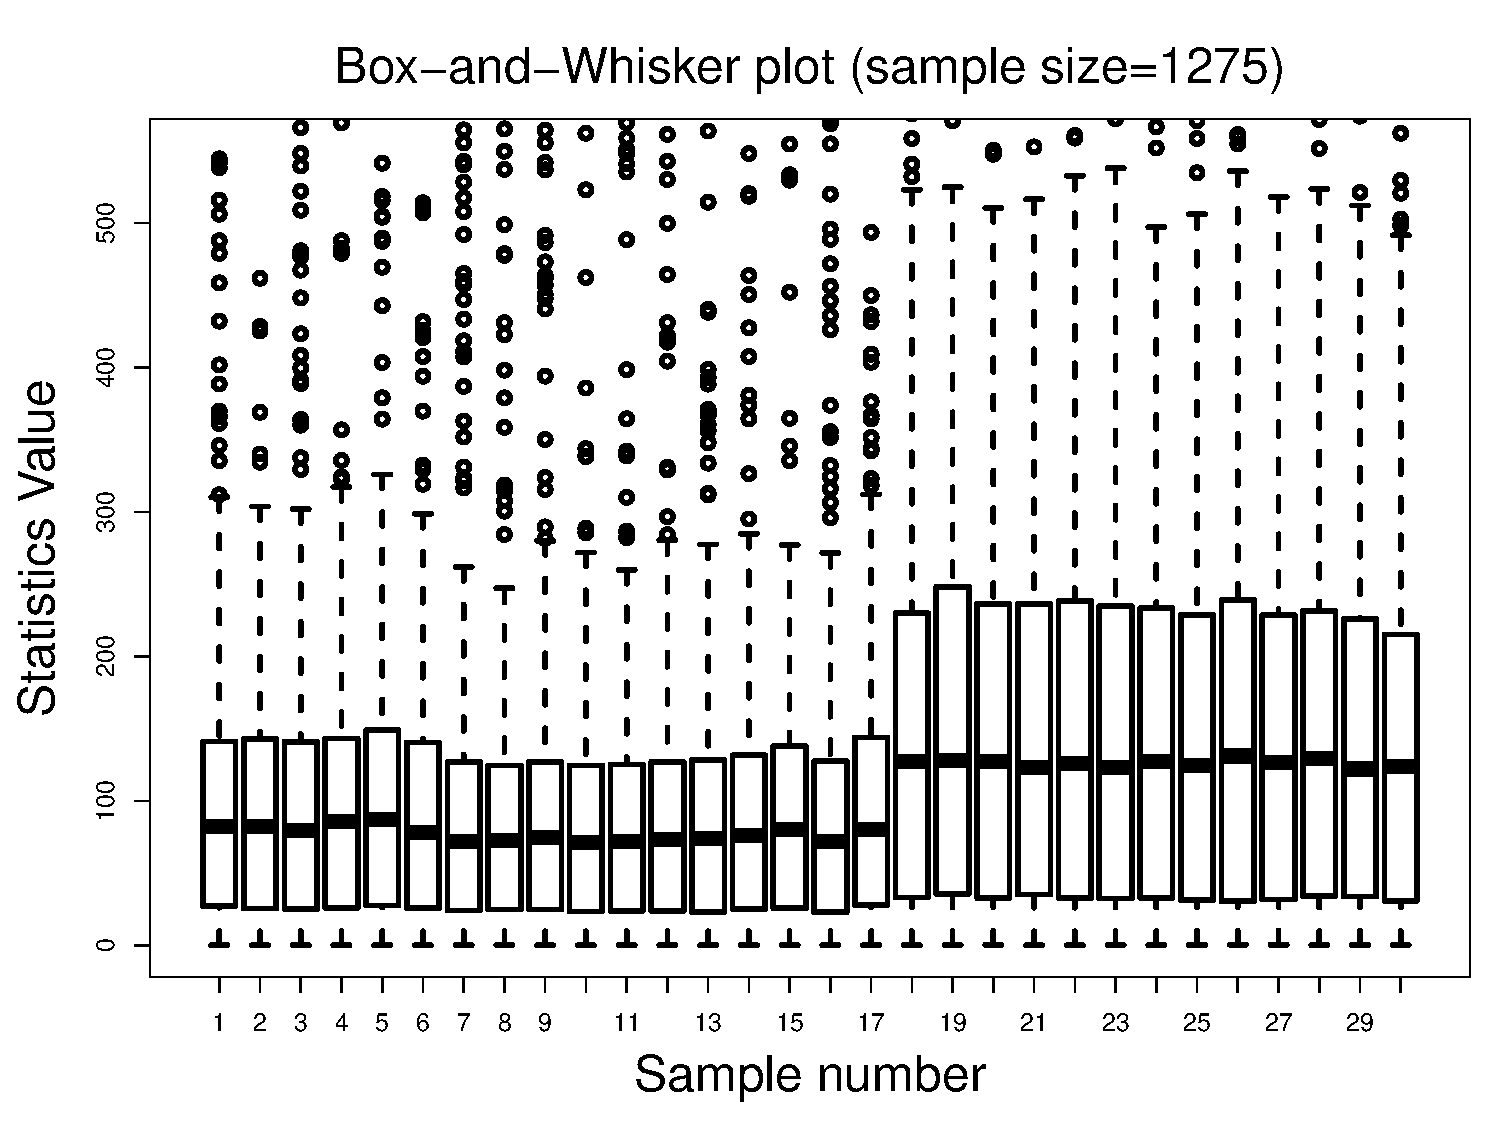
\includegraphics[width=0.45\textwidth]{pics/cfb_paper/OMF/OMFboxplot}
\caption{Box plot representing mean, lower and upper quartiles, maximum and minimum values for each of the sliding window.}\label{figure20}
\end{figure}

We could set some arbitrary limits bigger than $3\sigma$, but this may lead to overfitting if we try choosing the most appropriate limits repeating the trial and error cycles.
One way to address this problem is to handle outliers and to perform a set of a statistical test for each of the points~\cite{BakkerSensorsKDD09}.
Another way is to find a feature which is sensitive only to changes of a particular kind.
For example we can use as a feature a cumulative mean, i.e.\ average values of the signal from the beginning to the current point (Figure~\ref{figure21}).

\begin{figure}[htb!]
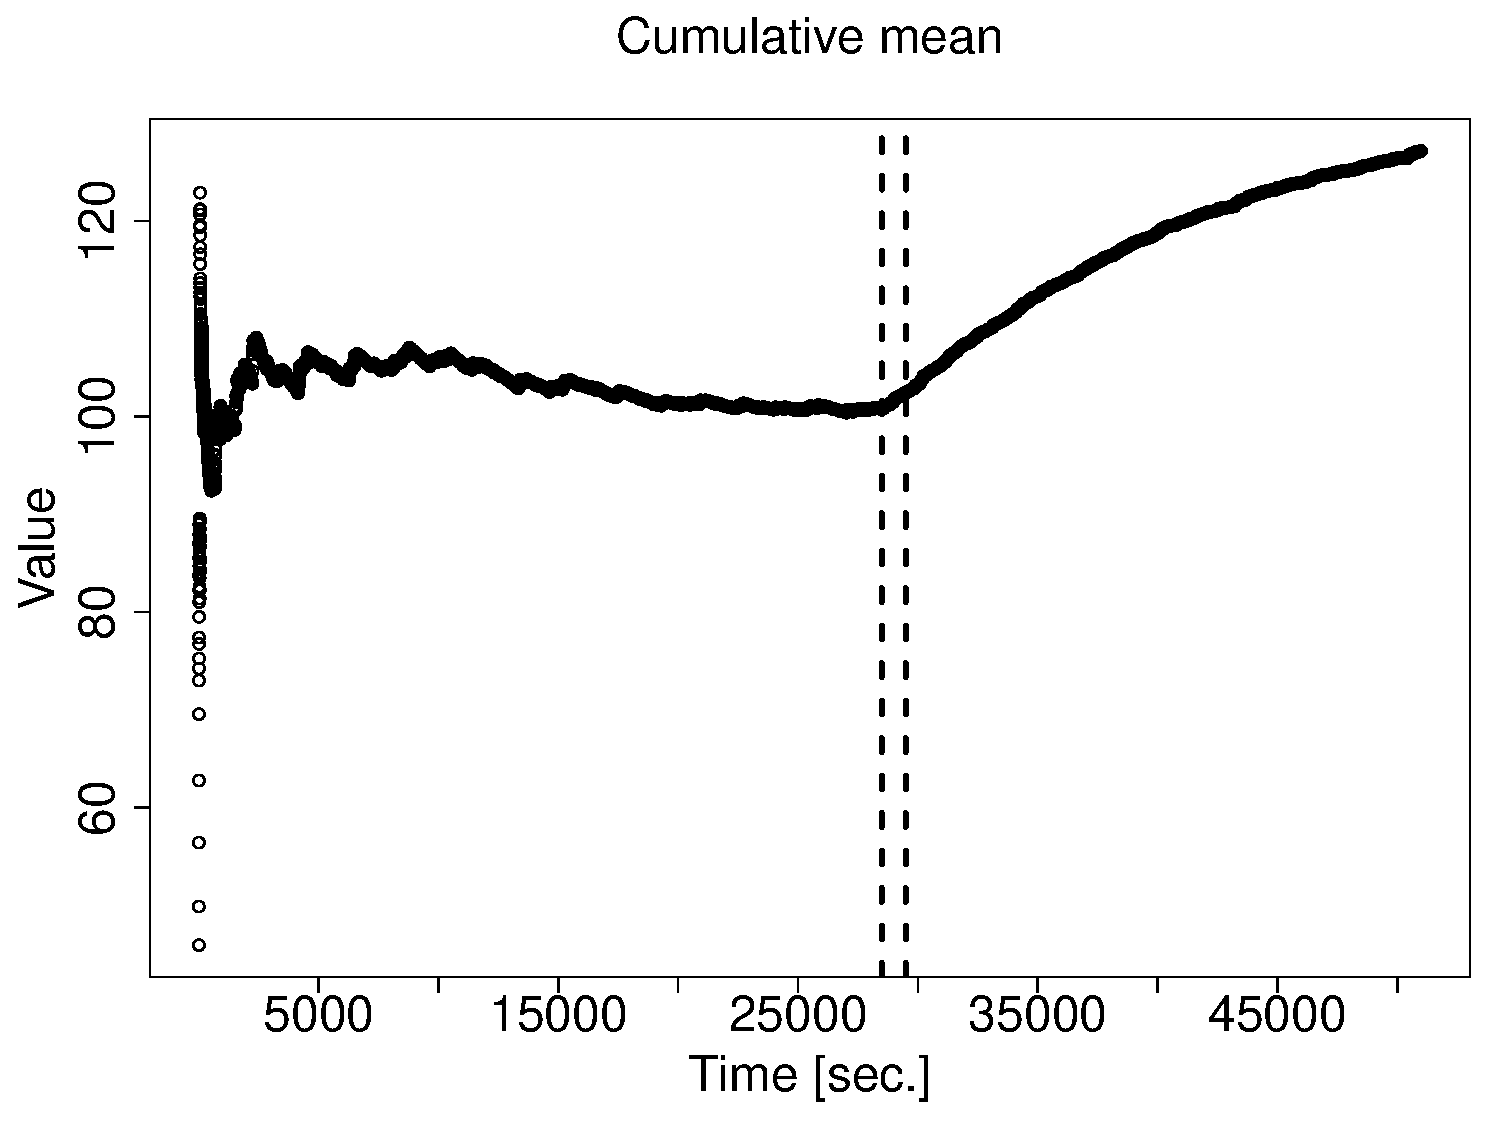
\includegraphics[width=0.45\textwidth]{pics/cfb_paper/OMF/OMFcumulativemean}
\caption{Cumulative mean}\label{figure21}
\end{figure}

In this case we can control cumulative statistic by control charts and in case of change we should calculate
this statistic from the last change point. Of course such method is computationally expensive but it is a cost to pay for the presence of the
noise and outliers.

Fortunately, QI computed on the same subset of points (from beginning of a signal to the current point) is much more resistant to outliers and noise presence.
Each time when change is detected we compute QI from the last change.
There are two parameters: the difference of logarithms of the current and the preceding values of QI and the minimum distance between changes.
With short data series, QI statistic gives statistically incorrect results.
Updates of QI were performed at the points marked by the vertical lines (Figure~\ref{figure22}).

\begin{figure}[htb!]
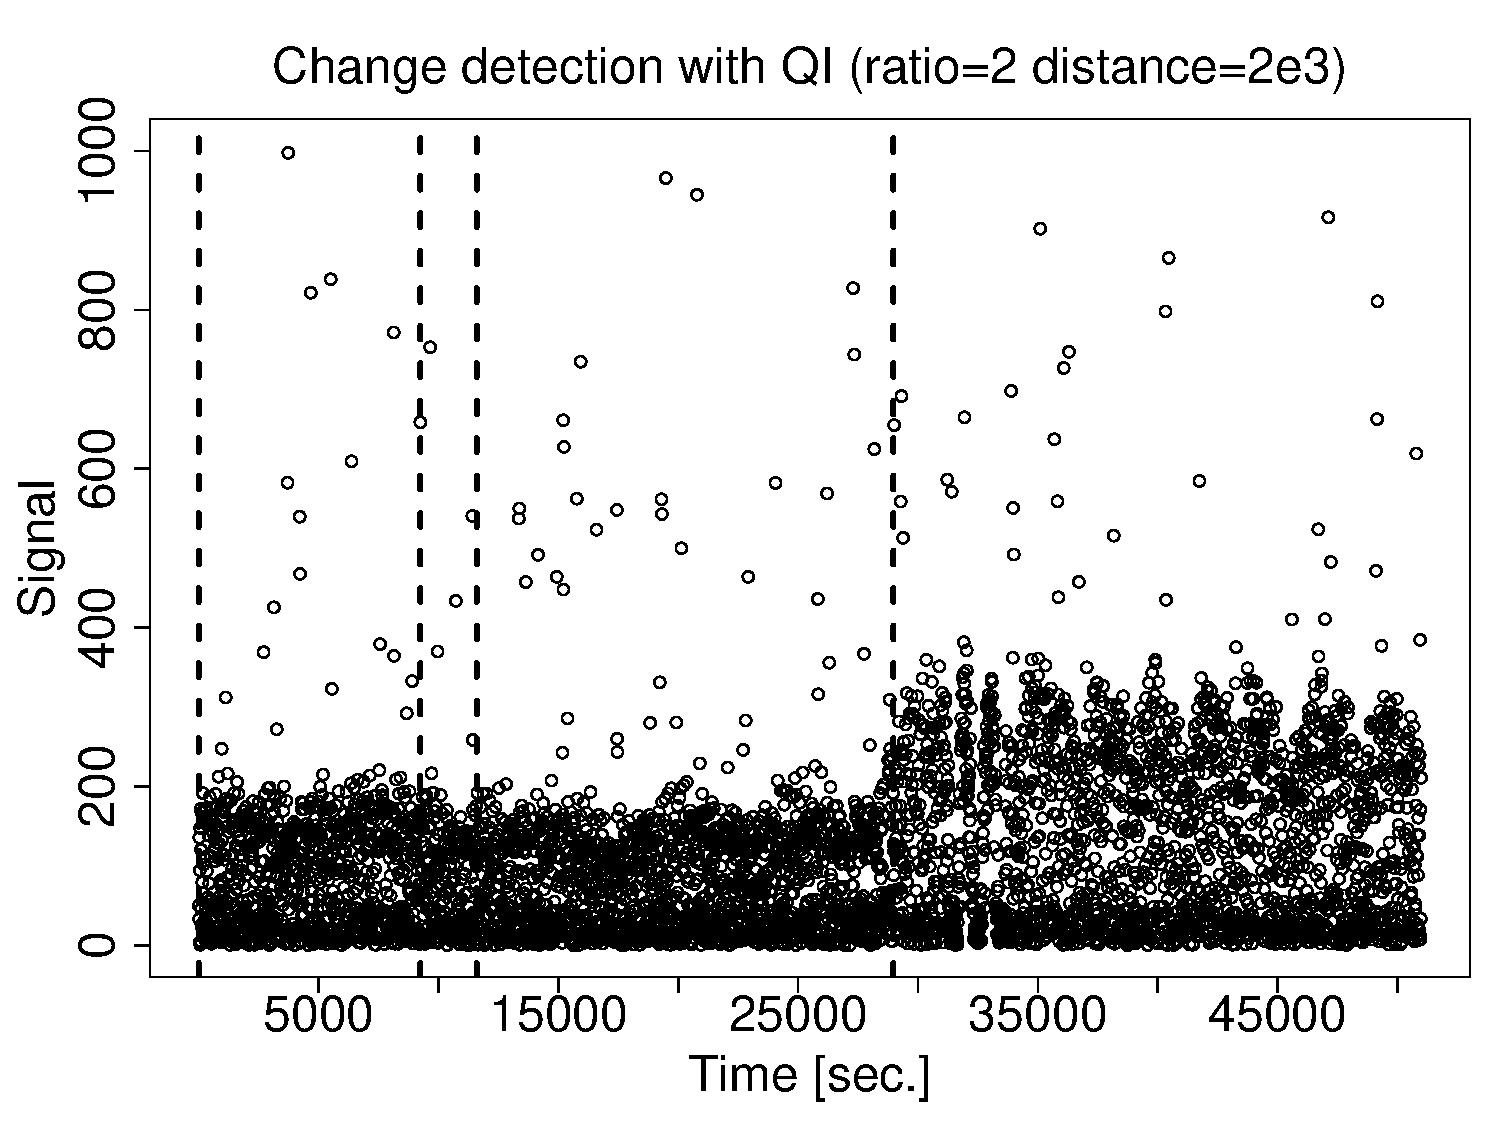
\includegraphics[width=0.45\textwidth]{pics/cfb_paper/OMF/OMFsteadyQI1}
\caption{Change points detected by means of QI which were calculated from the beginning of a signal initially and
after each detected change later. Detected points:(9236,11597,28973)}
\label{figure22}
\end{figure}

\paragraph{Detection with Density Ratio Estimation} 
Computing the density ratio estimation in the online settings (eq.~\ref{KDEformula}) we obtain change points presented in Figure~\ref{figure23}.
Actually, a series of changes is detected, but they all are concentrated near three mean points which are depicted by dashed lines.

\begin{figure}[htb!]
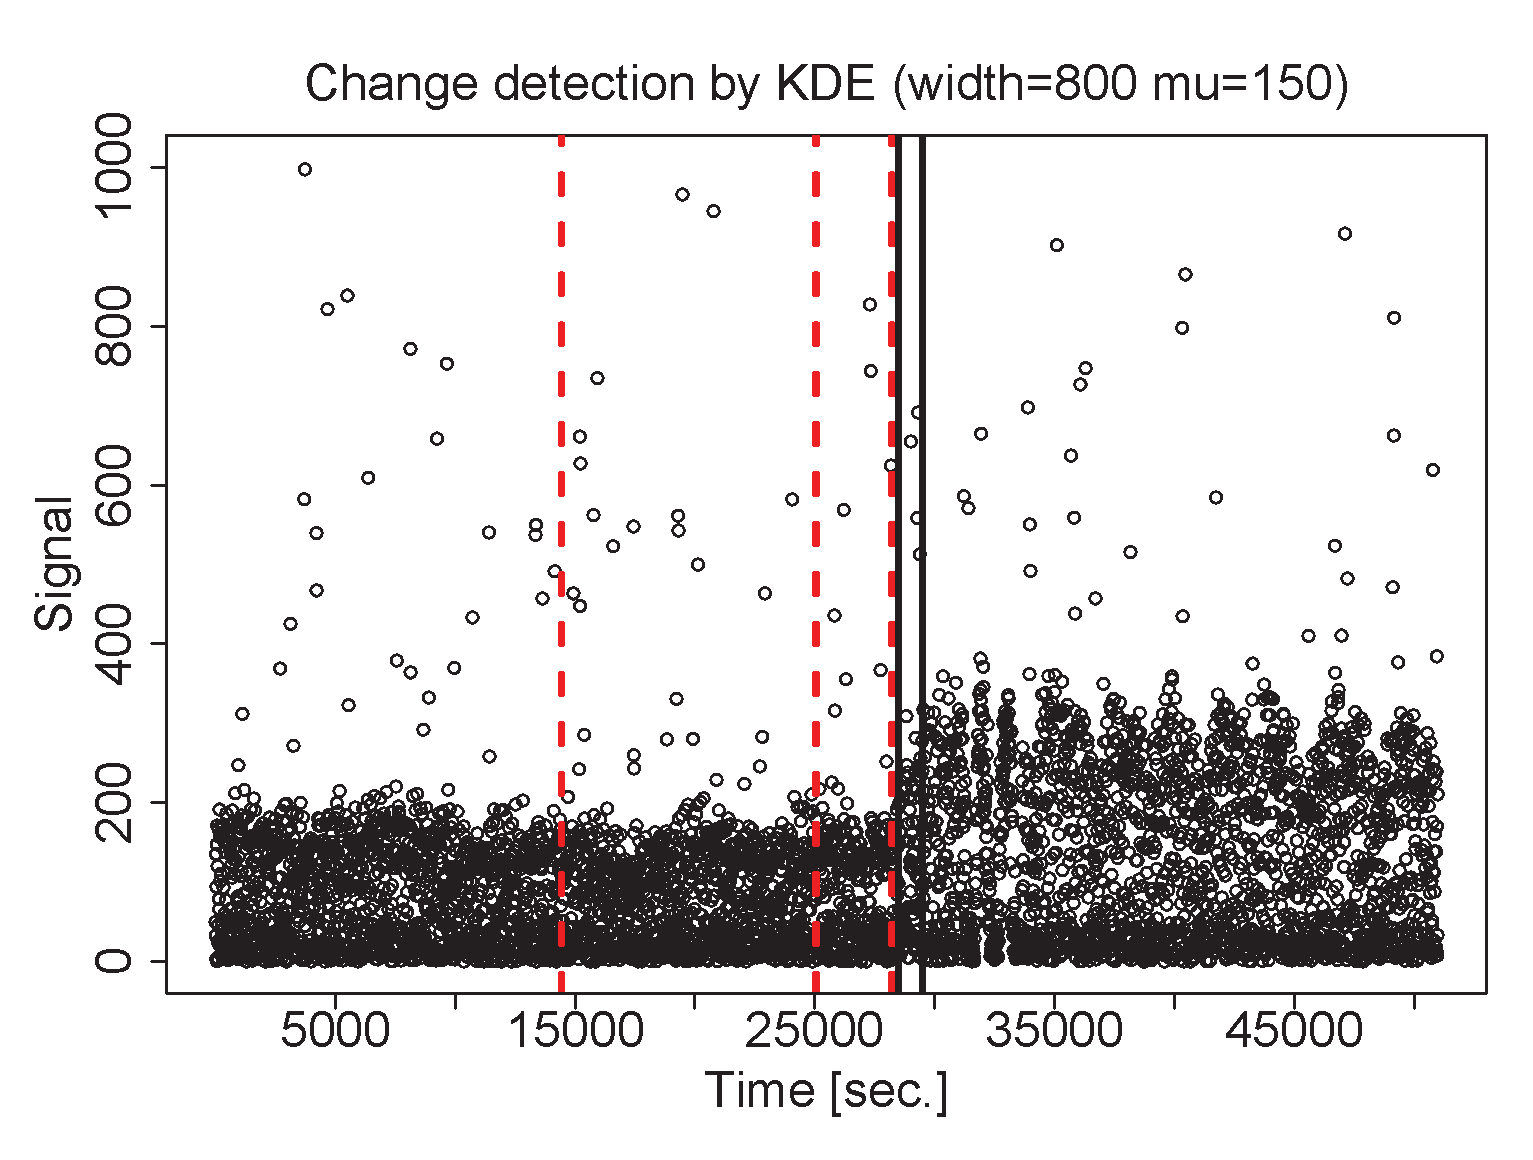
\includegraphics[width=0.45\textwidth]{pics/cfb_paper/OMF/OMFkde}
\caption{Change points detected by means KDE. Detected points:(14434,25061,28246). Successfully detected the main change at 28500 sec.} \label{figure23}
\end{figure}

\section{Conclusions}
\label{sec:conclusion}
We found a simple and intuitive approach for gradual and abrupt change detection in a noisy sensor data. 
Often sensor data needs to be preprocessed before applying change detection algorithms. For example noise and outliers should be removed.
QI-based change detection can handle gradual and abrupt changes without such preprocessing.

QI shows a good performance if the scale of a change in the mean or standard deviation
is comparable to the distance between quantiles in a test window by which we determine values of QI. 
We should note that QI shows good results for various types of changes only if sufficiently large amount of change free data from the past is available.
This is a property of the cumulative statistic.

We applied our approach for the sensor data collected from two devices modelling operation of an industrial CFB boiler. 
We analyzed different phenomena: particle size distribution and bed mass rapid change, subsequent mixture of two substances with a different PSD and mixing screw frequency change.

In the first case we had one abrupt change at the moment of adding particles with another PSD and after that the gradual
change due to mixing was following. Both kinds of changes were successfully detected by control charts, by on-line KDE and by the proposed QI method.
In the second case we attempted to detect gradual change in the fuel mass flow in a bunker, which was caused by an abrupt changes in the frequency of the mixing screw. This change was detected by means of QI and KDE.
For an abrupt change the results were similar to the case when the change happened due to the mixture of particle of different sizes.
It is interesting to note that as an aside result we found also another approach for online fuel mass estimation computing the lowest quantile.

Given these promising experimental results with QI for change detection, we plan to investigate QI further and study its behavior in a more formal and elaborate way.

\section{Acknowledgements}
This research is partly supported by Finnish Funding Agency for Technology and Innovations (TEKES) On-line CFD project and the Netherlands Organization for Scientific Research (NWO) HaCDAIS project.
Simulated sensor data were provided by VTT Research Centre of Finland.
We would like to thank R Development Core Team~\cite{Rref} and Luca Scrucca~\cite{qcc} for the open source software used in this study, \r{A}bo Akademi and Alf Hermansson for valuable technical support.




\chapter{Article: ACLAC}
Article: ACLAC: An approach for adaptive closed-loop anesthesia control

\begin{abstract}
In current practice, to control the anesthetic process, the
anesthetist delivers drugs according to the surgery procedure and
% which the patient is undergoing
% , to the patient characteristics, and to the current patient state.
to the current patient characteristics and state.
%
This is an open-loop procedure requiring an active participation of
the medical expert.
%
We propose an adaptive closed-loop controller for the regulation of
hypnosis for patients undergoing general anesthesia.
%
One of the main problems arising when designing such a controller is
related to the intra- and inter-patient variability.
%
We employ a simple regression model to make prediction of patient's
response and to compute the adequate doses of propofol to keep the
patient in the specified Bispectral Index target.
%
To make our model adaptive, we continuously monitor the patient
behavior and detect changes in patient response to update the
identification model.
%
Experimental evaluation on real patients data shows that we can
effectively detect change points. Simulation of the adaptive
closed-loop control with the change detection mechanism also suggests
that the use of the adaptation mechanism improves the control. 
%and can be investigated further in the hospital settings.
\end{abstract}
%-------------------------------------------------------------------------
\section{Introduction}
The main variables appearing in anesthesia are hypnosis, analgesia and
muscular relaxation. Hypnosis refers to the level of unconsciousness
of the patient. Analgesia is related to the level of insensibility to
pain. And muscular relaxation is also a variable of interest to avoid
movements during the surgical procedure and to make easier access to
patient’s organs.

In the anesthetic process, the clinician must guarantee an adequate level for these three variables.
% ... CHANGED TO:
% To achieve this, the anesthetist delivers drugs according to the surgery procedure to which the patient is undergoing,
% to the patient characteristics, and to the current patient state.
% ... TO:
% To achieve this, the anesthetist delivers drugs according to the surgery procedure, to the patient characteristics and state.
% %
% Traditionally the anesthetist starts with the infusion of these drugs according to well established protocols and then
% modifies the infusion depending on the clinical signs observed during the procedure.
Traditionally the anesthetist starts with the infusion of the drugs according to well established protocols and then
modifies the infusion depending on the patient characteristics and state.
%
%... Compressed:
% As can be observed this is an open-loop procedure, and
% only appears through the clinical observations of the medical expert.
%... To:
As can be observed this is an open-loop procedure.

During last years the introduction of closed-loop methodologies in
this field has been a matter of study and some closed-loop strategies
have been reported with real patients in the operating theater. These
approaches propose to consider both signal-based
~\cite{mendez_adaptive_2009,reboso_design_2012} and model-based
control schemes ~\cite{liu_closed_loop_2011, nino_epsac_controlled_2009}.
%
Most of them are focused in the regulation of the hypnosis level of
the patients once they become unconscious.
% COMPRESSED: (DELETED)
% The regulation of the
% analgesia level is quite more difficult due to the non-availability of
% a reliable index to measure the analgesic state.
%
% DELETED: "However, "
The hypnosis level can be measured through an index extracted
from the electroencephalogram (EEG). This variable is called
Bispectral Index (BIS)~\cite{bis} and is well correlated with the
level of unconsciousness. %related work on this is missing, i.e. we need to position wrt this existing work

We propose an adaptive closed-loop controller for the regulation of
hypnosis for patients undergoing general anesthesia and
% COMPRESSED (REMOVED): : because the same words are used further in second section - The problem of anesthesia control.
% One of the main problems arising when designing such a controller is
% related to the intra- and inter-patient variability.
% DELETED: "We"
employ a simple regression model to make prediction of patient's
response and to compute the adequate doses of propofol to keep the
% DELETED: (Bispectral Index) ADDED: "value"
patient in the specified BIS value target.
%
To make our model adaptive, we continuously monitor the patient
behavior and detect changes in patient response to update the
identification model.

The rest of the paper is organized as follows.
% NOT CHANGED
In Section~2 we introduce the problem of anesthesia control and emphasize the challenges to be addressed.
% TO:
%In Section~2 we introduce the problem of anesthesia control.
%
In Section~3 we present ACLAC -- our approach for adaptive closed-loop
anesthesia control that has a change detection mechanism built into
it. In Section~4 we discuss the results of the experimental study
including the simulation of the closed-loop anesthesia control on the
simulated data and the performance of the change detection on the real
data collected from ten different patients during in the surgery room.
Experimental evaluation on real patients data shows that we can
effectively detect change points. Simulation of the adaptive
closed-loop control with the change detection mechanism also suggests
that the adaptation mechanism is adequate and can be investigated
further in the hospital settings. Section~5 concludes with the
discussion of the limitation and future work.

\section{The problem of anesthesia control}
This work focuses on the regulation of hypnosis for patients undergoing general anesthesia.
% ADDED:
As a feedback variable for a close-loop control of a hypnosis we use the BIS signal.
%
In particular we considered a BIS target of 50~\cite{luginbuhl,rampil}.
%
The hypnotic drug used is intravenous propofol.
%
The control objective is to maintain the BIS in 50 rejecting the disturbances affecting
the patient during the procedure: surgical stimuli, blood loss, incisions, etc.

%
BIS variable is adimensional and varies between 100 (awake state) and 0 (no electrical brain activity).
%
% Compressed(removed):
% Different bands can be defined according to the state of the patient.
%
% Compressed:
% Thus, the values of BIS between 60 and 40 define the band for general
% anesthesia.
% To:
The values between 60 and 40 define the band for general anesthesia.
%
% Compressed:
% The availability of the BIS signal make it feasible to propose a
% close-loop control for hypnosis using this variable as the feedback
% variable.
% To:
% We propose a close-loop control for hypnosis using this variable as the feedback variable.

% CHANGED:
% One of the main problems arising when designing the controller is
% related with the patient variability.
% TO:
One of the main problems arising when designing the controller is
the patient variability.
%
We can distinguish both inter-patient and intra-patient
variability. Inter-patient refers to the variability appearing in the
response to the drug between different patients.
%
% COMPRESSED:
% And intra-patient variability appears because during surgery the
% response of the same patient along the procedure is changing with
% time.
% TO:
And intra-patient variability appears because of change in the
response during surgery of the same patient along the procedure.

% Removed: "Thus, one.."
An important specification that the closed-loop controller must
satisfy is the robustness to this variability.
%
From the control engineering point of view, two different approaches
can be used.
%
The basis of robust control is to design a fixed controller that
offers satisfactory performance even if the patient response
changes.
%
A different option is the use of adaptive controllers that includes
adaptation mechanism to change in response to changes in the patient.

In this work, we propose a predictive adaptive controller that
continuously monitors the patient behavior, propose a model to make
prediction of his response and computes the adequate doses of propofol
to keep the patient in the specified BIS target.

The sample time considered is 5 seconds. Although, according to
patient response, a bigger value can be considered, this sample time
is large enough to guarantee the applicability of the controller in
terms of computational burden.

\section{Approach}
Our approach consists of three main components: adaptive patient
modeling, control and change detection mechanisms that we describe in
the corresponding subsections.

\subsection{Adaptive modeling of hypnosis}
%As commented above, a predictive controller was designed using an adaptive patient model.
The common approach to model the patient dynamics to propofol infusion
is the use of compartmental models. %ref to compartmental models is missing
This approach considers different compartments interconnected and with
a given time constant. Drug is infused in the main compartment, and
from then is transferred to the other compartments until equilibrium
is reached between all the compartments. A common approach considers
four compartments (central, slow, fast and \textit{effect
  site})~\cite{schnider_influence_1998}.
%
The BIS variable can be obtained as a nonlinear function of the
concentration in the effect site compartment.

We use a linear approximation to this model using an Autoregressive
with exogenous input (ARX) model that computes the input signal at
sample instant $d$ as a function of the input and output values at
previous time instants. The computation of the model parameters is
done online by using a least squares minimization algorithm.
%
%   COMPRESSED(REMOVED):
%
Consider the following polynomials:
\[
A(z^{-1})=1+a_{1}z^{-1}+a_{2}z^{-2}+...+a_{na}z^{-na}
\]
\[
B(z^{-1})=b_{0}+b_{1}z^{-1}+b_{2}z^{-2}+...+b_{nb}z^{-nb}
\]
\noindent
% deleted: where $na$ and $nb$ are the degrees of the polynomials and $z^{-1}$ is the \textbf{delay operator}.
where ${na}$ is the number of previous \emph{outputs} and ${nb}$ is the
number of previous delayed by $n_{d}$ \emph{inputs} on which the
current output depends and $z^{-n}$ is the \emph{delay operator}
which is defined by $z^{-n}x(t)=x(t-n)$.  Then, the ARX model for the
BIS variable can be expressed as:
\[
A(z^{-1})BIS(t)=B(z^{-1})u(t-n_{d})+e(t)
\]
\noindent
% http://www.ncbi.nlm.nih.gov/pubmed/8695136
% variable-rate propofol infusion up to 0.15 mg/kg/min
where $BIS(t)$ is the $BIS$ value at $t$, $u(t)$ represents the propofol infusion rate in $mg/l/min$, $e(t)$ is the residual
error and $n_{d}$ is the input-output delay.
Thus, the model can be expressed as:
\begin{multline}
BIS(t)+ a_{1} BIS(t-1)+...+ a_{na} BIS(t-na) = \\
b_{0}u(t-n_{d})+ b_{1}u(t-n_{d}-1)+...+ b_{nb} u(t-n_{d}- n_{b})+e(t)
%\label{eq:model}
\end{multline}
% % Added:
% where $\pmb{na}$ is the number of previous \textbf{outputs} and $\pmb{nb}$ is the
% number of previous delayed by $\pmb{n_{d}}$ \textbf{inputs} on which the
% current output depends.
% %
% $BIS(t)$ is the $BIS$ value at $t$, $u(t)$ represents the  propofol infusion rate in $mg/l/min$, $e(t)$ is the residual error.
%
% COMPRESSED:
% The choice for $na$, $nb$ and $n_{d}$ was done using simulations.
% In this work we use $na=nb=4$ and $n_{d}=1$.
% TO (ADDED: "least squares algorithm"):
The estimation for $na=nb=4$ and $n_{d}=1$ was done using least squares algorithm during simulations.
%
% COMPRESSED (REMOVED): : The same appears earlier as: "The computation of the model parameters is done by using a least squares minimization algorithm."
% We use an online least squares algorithm to compute the A and B
% polynomials using past information of the process.
%
% COMPRESSED REMOVED "Thus.":
The model will adapt to the specific patient response and to eventual changes in its dynamics.
% not changesd TO:
% The model will adapt to the patient response and to changes in its dynamics.
%
Figure~\ref{fig:ARXmodel} shows the identification scheme used.

\begin{figure}[htb!]
\centering
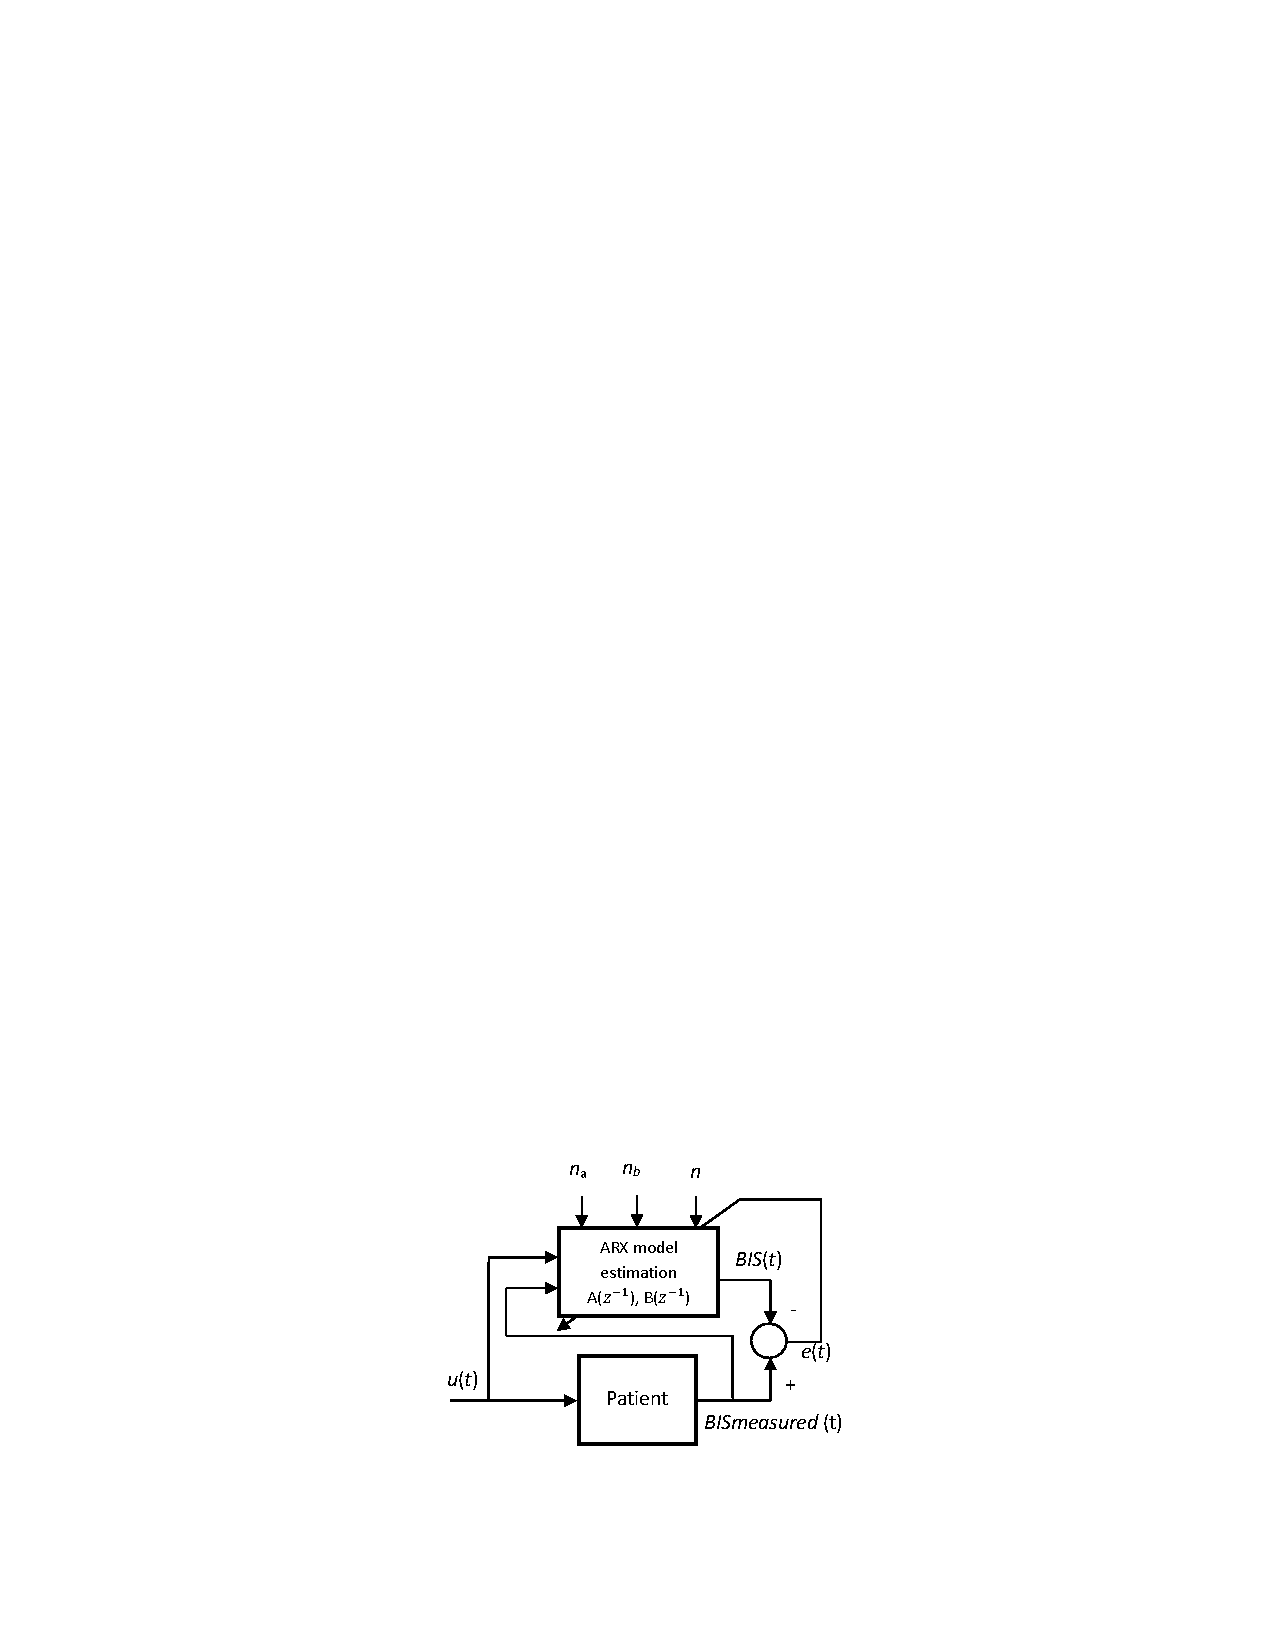
\includegraphics[width=0.4\textwidth]{./articles/pics/aclac_paper/ARXmodel.pdf}
\caption{Patient model identification.} %scheme
\label{fig:ARXmodel}
\end{figure}

% CHANGED:
% The initial model chosen for the patient is a standard model obtained from the analysis of a set of real patient data.
% TO:
The initial model for the patient is estimated from the analysis of a set of real patient data.
%
After the initial training, the adaptation algorithm proposes a new
model based on real data of the patient. This model is regularly
updated along the time.

% CHANGED:
% One important issue to improve the accuracy of the model
% identification scheme is the availability of information of patient
% changes.
% TO:
% The availability of information of patient changes can improve the
% accuracy of the model identification scheme.
% CHANGED:
% This information would be used in the identification subsystem to make
% decisions about the relevance of the patient data used in the
% identification algorithm.
% TO: DELETED:""
% This information would be used in the identification subsystem to make
% decisions about the relevance of the patient data used in the identification algorithm
% CHANGED TO:
The availability of information of patient changes can improve the
accuracy of the model identification scheme which would be used to
% DELETED: identification
make decisions about the relevance of the patient data used in the algorithm.
% Thus, one contribution of this paper is the inclusion of a change
% % DELETED " eventual" from " eventual changes"
% detection algorithm to detect changes in patient response and use it to improve the identification performance.
% TO:
Thus, one contribution of this paper is the inclusion of a change
detection mechanism to detect changes in patient response.
%improve the identification performance. - mentioned in the previous sentence
%
% DELETED : "simply"
In ACLAC we disregard data preceding to a detected changepoint.
This way, the model update will only include information of the new dynamics of the patient.
%This scheme will improve the performance obtained with adaptive schemes based in fixed time window.

\subsection{Control approach}
The controller proposed to regulate the hypnosis of the patient is shown in Figure~\ref{fig:Controller}.
%
% COMPRESSED:
% As can be observed the model predictive controller(MPC) decides the adequate profofol infusion rate to be infused to the patient.
% TO:
The model predictive controller(MPC) decides the adequate profofol infusion rate to be infused to the patient.
%
The MPC uses a linear model for the predictions that is obtained from the model identification module.
%
% COMRESSED: : REMOVED - "As commented,"
The change detection algorithm provides information to the identification scheme that is used to determine the time-window of
past data used.
\begin{figure}[htb!]
\centering
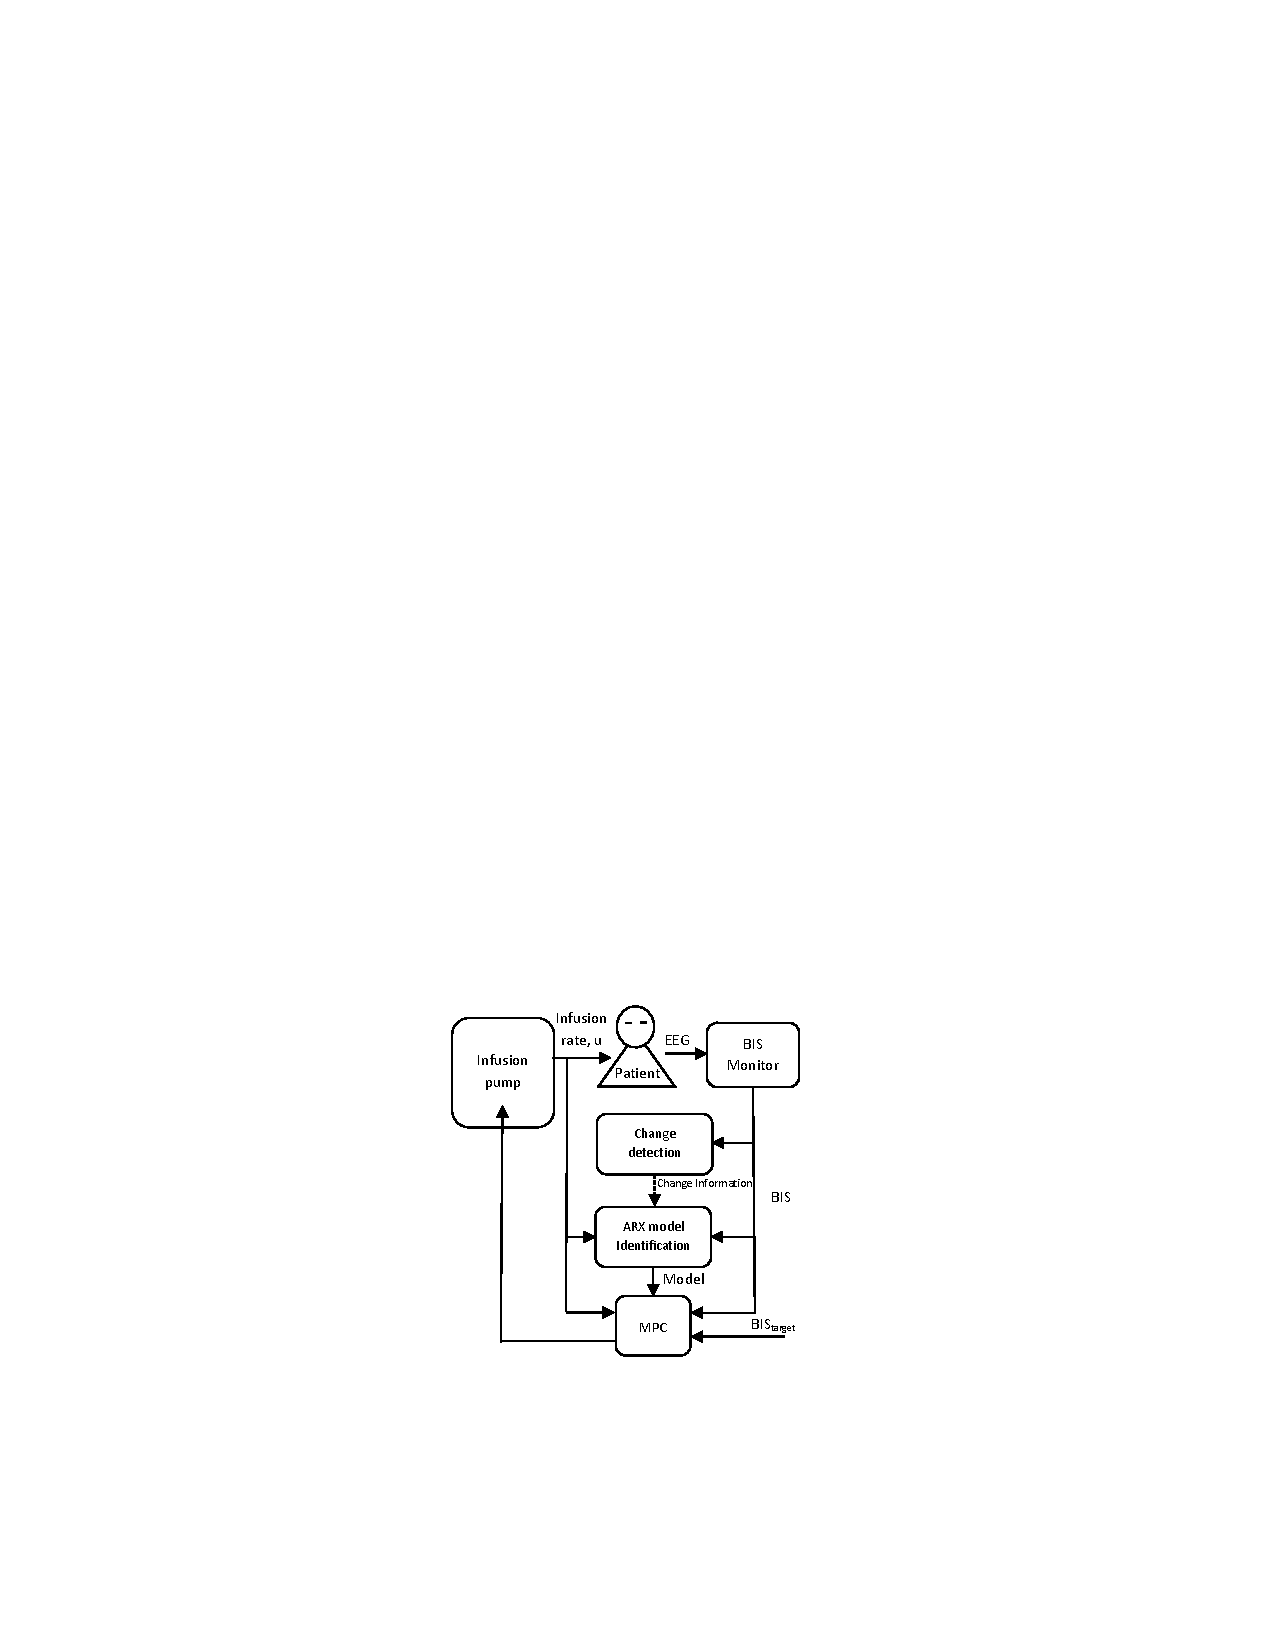
\includegraphics[width=0.40\textwidth]{./articles/pics/aclac_paper/Controller.pdf}
\caption{Closed-loop control scheme using identification scheme with change detection.}
\label{fig:Controller}
\end{figure}
% Model predictive control
% CHANGE: "consists of" to "includes"
MPC controller includes an optimization process in which the best
future inputs are computed based on the minimization of a given
function costs. The cost function uses predictions obtained with the ARX model.
% CHANGE: DELETED: "provided by the identification subsystem."

The formulation of the problem can be done as follows~\cite{Bordons}:
%\begin{equation}
\begin{multline}
\min\limits_{u(k|k),...,u(k+p-1|k)} \sum_{i=1}^{p} w_{i}(BIS(k+i|k)-BIS_{\textit{target}})^2 \\
+ \sum_{i=1}^{c}r_{i}\Delta u (k+i-1|k)^2
\end{multline}
subject to % equation~\ref{eq:model}.
\begin{multline}
%BIS(t)+a_{1}BIS(t-1)+...+a_{na}BIS(t-na) = \\
% b_{0}u(t-n_{k})+b_{1}u(t-n_{k}-1)+...+b_{nb}u(t-n_{k}-n_{b})
BIS(t)+a_{1}BIS(t-1)+...+a_{na}BIS(t-na) = \\
 b_{0}u(t-n_{d})+b_{1}u(t-n_{d}-1)+...+b_{nb}u(t-n_{d}-n_{b})
\end{multline}
\begin{multline}
BIS_{max} \ge BIS(k+i|k) \ge BIS_{min}, i=1,...,p \\
u_{max} \ge u(k+i-1|k) \ge u_{min}, i=1,..,c \\
\Delta u_{max} \ge \Delta u(k+i-1|k) \ge -\Delta u_{max}, i=1,..,c
\end{multline}
\noindent
where $k$ is the current time instant, $p$ and $c<p$ are the sizes of
the prediction horizon and control horizon respectively,
$BIS_{target}$ is the target for the $BIS$, and $u(k+i-1|k)$,
$i=1,...,p$, is the set of future input values, where
\begin{multline}
u(k+i|k)=u(k+c-1|k), i=c,...,p-1 \\
\Delta u(k+i-1|k)=u(k+i-1|k)-u(k+i-2|k)
\end{multline}
The optimization problem is solved at time instant $k$. Under this
approach, the control law for $u(k|k)$ is obtained by solving a
quadratic programming problem. The optimal input $u(k)=u_{opt}(k|k)$
is applied to the plant. This process is repeated in subsequent times
$k+1, k+2$, etc.  Thus the new control law $u(k +1|k +1)$ may be
different from the control signal calculated above. This principle is
called moving horizon strategy.
%----------------------------------------------------------------------%
%-------------------- CHANGE DETECTION METHOD -------------------------%
%----------------------------------------------------------------------%
\subsection{Change detection method}
\label{sec:ChangeDetectionMechanism}
%
The term change point stands for a phenomenon when statistical
properties of a data stream change significantly over time.
%
In medical sensor data streams we can observe changes of different
types: change in the mean value, variance, autocorrelation, in the
seasonal and trend components, etc. Changes can be classified also
with respect to the rate of the change into abrupt and gradual
changes. These changes, strictly speaking, are happening almost
continuously (depending on the `scales' of the changes which we
% DELETED "And" from "And one of the problems"
consider). One of the problems is to define rules by which we can
determine whether change is significant and should be detected
% DELETED: "(alerted)"
or not.
%
Such rules can be constructed using state-of-the-art change detection
methods based on control charts, cumulative sum (CUSUM,~\cite{Cusum}),
heuristic (thresholding) approaches, two sliding windows statistic
monitoring (w.r.t.\ data or modeling error), likelihood and density
ratio estimation for two competitive models among others~\cite{Nikiforov}.

We are interested in detection of the change in the mean value because
a BIS target value is 50 and control limits are defined by horizontal
lines of values 40 and 60.
% % COMPRESSED: REMOVED
% %is the following true?
% The most natural method for our task of change detection in BIS signal
% seems to be control charts or CUSUM method. In that case there is a
% need to define part of the signal which is `in control' and after that
% we can calculate control limits and ARL (Average Run Length) and other
% initial parameters values. But because of patient's inter- and
% intra-variability control limits and target value can slightly change
% between different patients or along the procedure for one patient.

In the domain of depth of anesthesia monitoring the problem of change
detection has been studied recently~\cite{GamaDecisionSupportSystems}.
A Page-Hinkley test with a forgetting mechanism (PHT-FM) was proposed
in~\cite{GamaRealTimeAlg}. This method is
on-line, %(unlike one used in our approach, which should be considered as `pseudo' on-line)
but it needs threshold value tuning that maybe not easy to achieve in
our case when dealing with noisy data or presence of outliers. Also it
requires the availability of training data on which the models can be
tuned.

%say, what the actual requirements are, e.g. wrt running time
%is the following true? none of the following is justified here
For our purposes we need a method which satisfies the following
conditions: 1)~it is applicable in an on-line settings, 2)~it is able to
detect multiple change points, 3)~it should take into account all
detected change points and decide on-line which of them should be
dropped because of the change in the scales of the changes.

% CHANGED:
%The commonly used approach for a single change point in a fixed interval is to perform likelihood ratio statistical hypothesis test.
% TO:
The commonly used approach for a single change point in a fixed interval is to perform likelihood ratio test.
%
In case of a single change point the null hypothesis $H_{0}$ is no
change point, alternative hypothesis $H_{1}$ is a single change point
at the moment of time $\tau$.
%
In other words, likelihood ratio test compares the fit of two
models, one of which is a special case of the other.
%
Given sequence of data $y_{1:n}=(y_{1},...,y_{n})$, it is said that
change point occurs at the moment of time $\tau$, such that the
statistical properties of $(y_{1},...,y_{\tau})$ and
$(y_{\tau+1},...,y_{n})$ are different accordingly to the chosen rules.
%
Twice the negative log-likelihood ratio function is used as a test
statistic to decide whether the change has occurred.
\begin{equation}
%ML(\tau_{1})=\log p(y_{1:\tau_{1}}| \hat{\theta_{1}}) + \log p(y_{(\tau_{1}+1):n}| \hat{\theta_{1}})
L(\tau)= \sum_{i=1}^{\tau}  \log p( y_{i}|\hat{\theta_{0}} ) + \sum_{i=\tau+1}^{n} \log p(y_{i}| \hat{\theta_{1}})
\end{equation}
\noindent
where $\hat{\theta}=(\mu, \sigma)$ is the maximum likelihood estimate of the parameters from likelihood function:
\[
\log p (y_{1:n}|\theta) =  -\frac{n}{2} \log(2 \pi) - \frac{n}{2} \log(\sigma^2) - \frac{1}{2\sigma^2} \sum_{i=1}^{n}(y_{i}-\mu)^2
\]
The test statistic is
\begin{equation}
\label{eq:gamma}
\lambda=C(y_{1:n}) = 2[\displaystyle \max_{\tau} L(\tau) - \sum_{i=1}^{n} \log p(y_{i}|\hat{\theta})]
\end{equation}
\noindent
%
where $\max\limits_{\tau} L(\tau)$ is the maximum log-likelihood
value under the alternative hypothesis.  The null hypothesis is
rejected if $\lambda > c$ where $c$ is selected threshold~\cite{KillickRpackage}.

In case of multiple change points the following function should be minimised:
\begin{equation}
\label{eq:optimal_partitioning}
\sum_{i=1}^{m+1}[C(y_{(\tau_{i-1}+1):\tau_{i}})] + \beta
\end{equation}
\noindent
where $m$ is the number of change points, $C$ is the twice negative
log likelihood cost function(Eq.~\ref{eq:gamma}) and $\beta$ is a
penalty term~\cite{KillickOptimalDetection} to prevent overfitting.
Value of $\beta$ was tuned during experiments.
%
%The term `changepoint' mostly refers to the situations when change is detected given fixed amount of data (moving interval during on-line monitoring) while the term `time-series segmentation' refers to algorithms which deal with a whole data set. During the segmentation data is split in such a way that we obtain the maximum difference (measured by the cost function) between emerged segments.
%
The combination of on-line monitoring algorithms and time-series segmentation methods is a promising approach for BIS monitoring because we often do not know in advance scales of the changes. Therefore, we have to perform analysis offline over detected points in order to discard (or keep) some of them if it is necessary.
%
For multiple change points detection we use PELT method
~\cite{KillickOptimalDetection}, which is based on dynamic programming
optimal partitioning algorithm proposed in~\cite{Barnes}.
%
Optimal partitioning algorithm performs recursive process that minimise function(Eq.~\ref{eq:optimal_partitioning}).
%
PELT method contains the pruning step within the dynamic
% DELETED: "significantly"
program which reduces computational cost of the method.
%
Comprehensive overview of the methods and description of the optimal
partitioning and PELT algorithms with pseudo-codes can be found in
~\cite{KillickOptimalDetection, KillickRpackage}.
%...........................................................%
%... EXPERIMENTAL STUDY / EVALUATION OF CHANGE DETECTION ...%
%...........................................................%
\section{Experimental study}
The validation of the proposed algorithm is done using real data
obtained from 10 patients undergoing general anesthesia. Patients are non
premedicated of ASA class I-II, scheduled for gynecological or
abdominal surgery with an estimated duration more than 30 minutes. A
laptop PC records both the BIS values and the infusion rate using
RS-232 links. The measurement of the BIS variable is done with a
{BIS-XP\texttrademark} monitor (Aspect Medical System) connected using
a RS-232 link and using four $ZipPrep^{\textregistered}$ electrodes. A
Graseby $3500^{\textregistered}$ infusion pump (Graseby Medical Ltd) with
propofol 1\% is the actuation system and was also connected via RS232
port to the PC. Sample time was 5 seconds.
% CHANGED:
% The data collected included both the induction phase and the maintenance phase.
% TO:
The data collected included both the induction and the maintenance phase.
%
In the induction phase a bolus dose is applied to take the patient
rapidly to the target area. In the maintenance phase the infusion rate
is calculated to keep the patient in the target BIS.

\subsection{Evaluation of change detection}
Change points for two signals are shown in
Figures~\ref{fig:ChangeDetection1}~and~\ref{fig:ChangeDetection2} (vertical dashed red lines).
%
% Totally, we considered signals from ten patients. % Mentioned at the beginning of section Experimental study.
%
The horizontal lines depict the target value and the general
anesthesia band.  In Figure~\ref{fig:ChangeDetection1} we can see that
the detected change points divide observations into four stages. The
first stage is short and has a high variance, but BIS is the in
control limits. In the second stage BIS is between the target value
and the upper limit. In the third stage BIS is below the target value,
but above the lower limit. In the fourth stage BIS is fluctuating
around the target value.  In Figure~\ref{fig:ChangeDetection1} we can
see that all out of limits periods are detected by the change
detection mechanism.

The detected change points represent 'changes' in a statistical
sense. It is described in subsection~\ref{sec:ChangeDetectionMechanism}.
Visual inspection of changes is difficult even for the domain experts.
Having no exact points on the BIS signals denoting ground truth
changes makes its hard to assess accuracy of detection in a
quantitative way.
% ?:
%Change points determine moments when regression model is updated using only relevant time windows.
\begin{figure}[htb!]
\centering
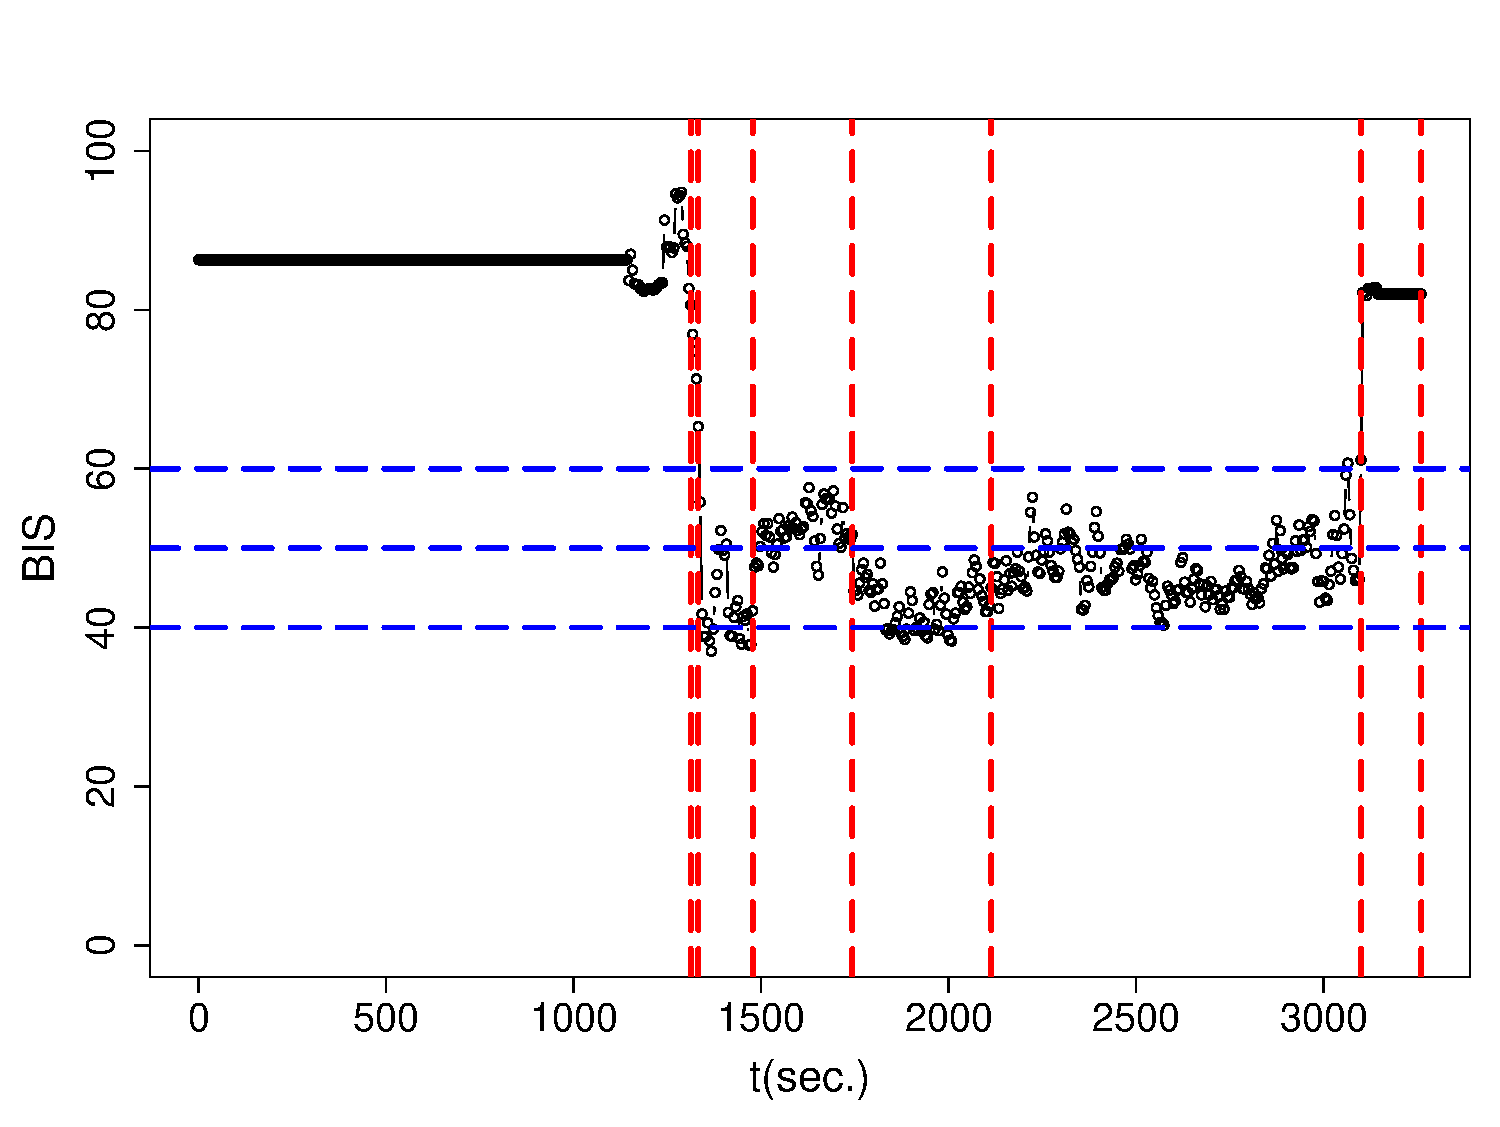
\includegraphics[width=0.40\textwidth]{./articles/pics/aclac_paper/ChangeDetectionImage4.pdf}
\caption{Four stages detected in BIS.}
\label{fig:ChangeDetection1}
% COMPRESS:
%\end{figure}
%\begin{figure}[htb!]
\centering
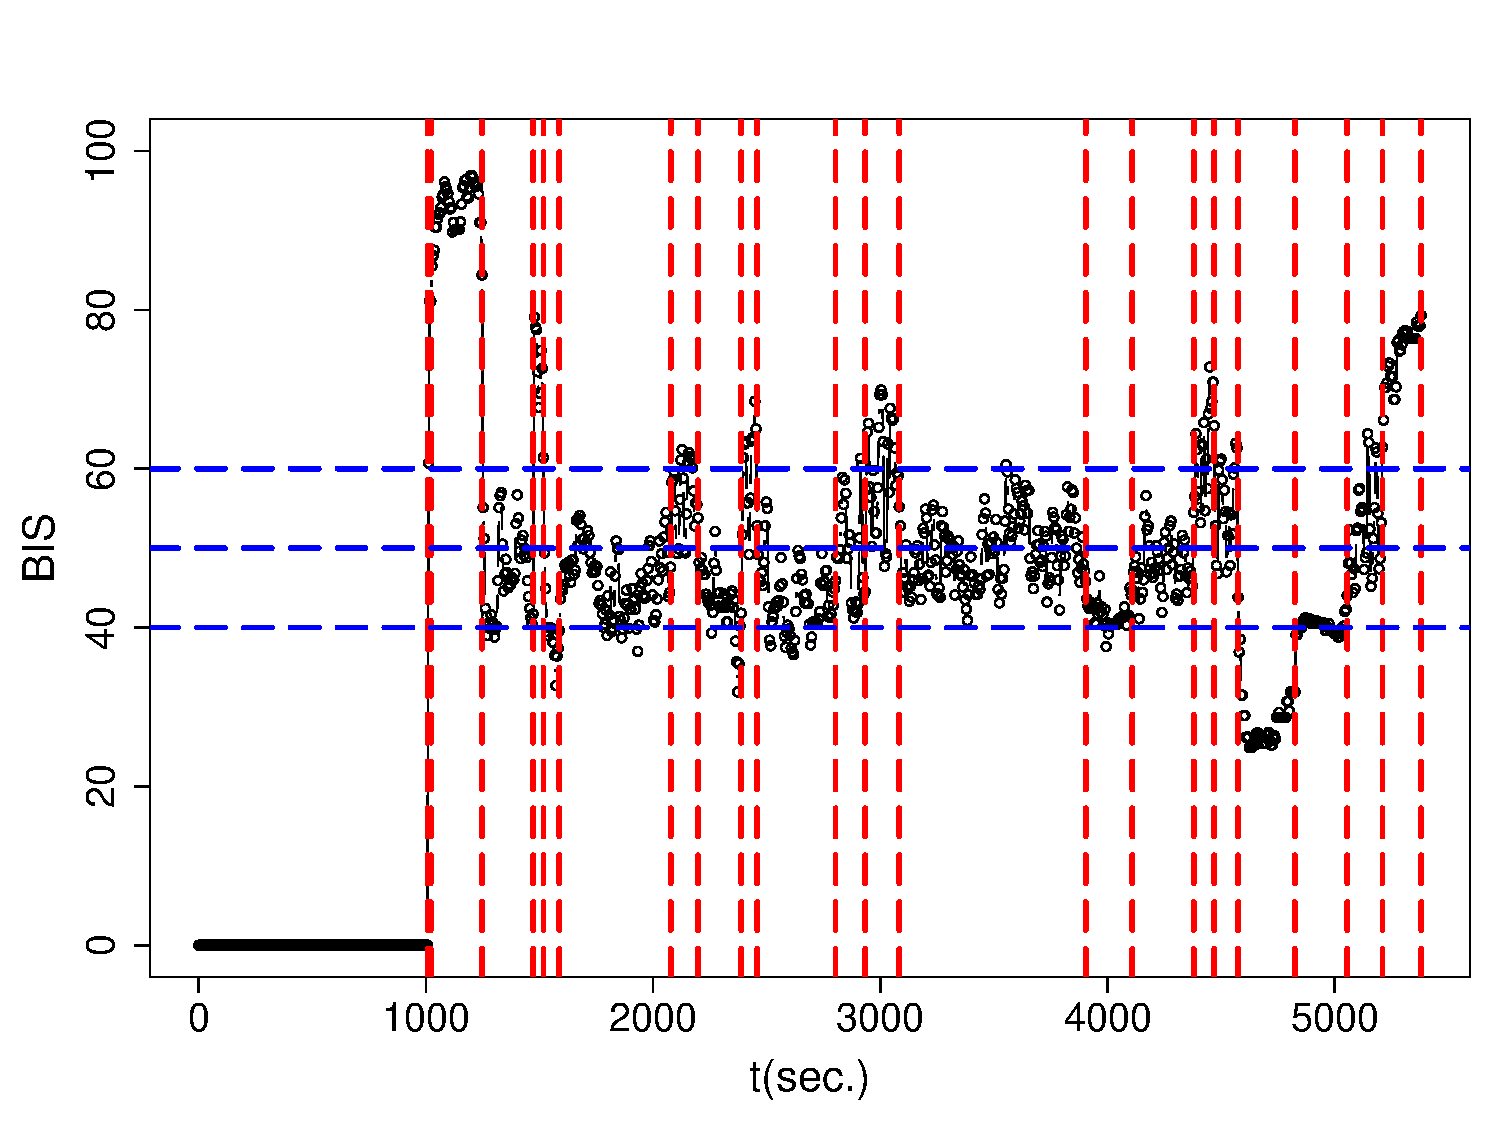
\includegraphics[width=0.40\textwidth]{./articles/pics/aclac_paper/ChangeDetectionImage6.pdf}
%\caption{Change detection in BIS with high variance.}
\caption{Case of BIS with high variance.}
\label{fig:ChangeDetection2}
\end{figure}
%...........................................................%
%........................ LIMITATIONS ......................%
%...........................................................%
%\subsection{Limitations of change detection mechanism}
%Change detection mechanism continuously monitors arriving data and
%performs inner loop to check if the current partition is the best
%given the new data. Algorithm finds the optimal partition of the
%$(n+1)$ data points using previously obtained optimal partitions for
%$(1,2,...n)$ data points~\cite{Barnes}.  That is why the location of
%the last change point may change or even dissappear when new data
%points arrive. It is confusing but reasonable because scales of
%changes are also changing over time. And it is also reasonable when we
%have a noisy data or when signal is highly unpredictable.
%...........................................................%
%............ CLOSED-LOOP CONTROL EVALUATION................%
%...........................................................%
\subsection{Closed-loop control evaluation}
% CHANGED:
% The evaluation of the proposed controller (Fig.~\ref{fig:Controller}) was done in simulation. The patient response was simulated using the
% Schnider compartmental model~\cite{schnider_influence_1998} for one standard patient(male, 70Kg, 175cm).
% TO:
The evaluation of the proposed controller Fig.~\ref{fig:Controller})
was done in simulation of the patient response using the Schnider
compartmental model~\cite{schnider_influence_1998} for one standard
patient(male, 70Kg, 175cm).

BIS target  is 50  and sample  time is 5 seconds. In the simulations
performed we replicate the procedure of the anesthetist. First a bolus
dose of $2mg/kg$ is infused  at maximum infusion rate and, after this,
the automatic mode starts.

Figure~\ref{fig:fig2ColsedLoopContrlSim} shows the results obtained with ACLAC.
%in a patient using the controller with change detection algorithm for model identification.
Two disturbances are considered in the patient
dynamics in $t = 20.8$ \emph{min} and $t = 33.3$ \emph{min}. The origin of these disturbances
can be surgical stimulus, blood loss, etc. The result is a change in
the patient state and in the patient model parameters.
% CHANGED: Removed - "Observe that "
Before these disturbances occur the controller is able to regulate the state of the patient to 50.
%
In the figure, the model predictions are
depicted in dotted line. As can be observed the prediction errors are low.
% CHANGED: "the change detection algorithm is able to detect" to "the change detection algorithm detects"
% ALSOE : Removed "as commented in previous section" from "as commented in previous section to improve"
When the disturbance occurs, the change detection algorithm detects a
change in the patient behavior and this information is used in the identification scheme to improve the identification.
%
% CHANGE: Removed "As can be observed"
The identification module does not update to a new model until it have data enough to guarantee correct model identification.
%
Thus, after the first disturbances arrives, the model update is done again at $t = 26.4$ \emph{min}.
\begin{figure}[htb!]
\centering
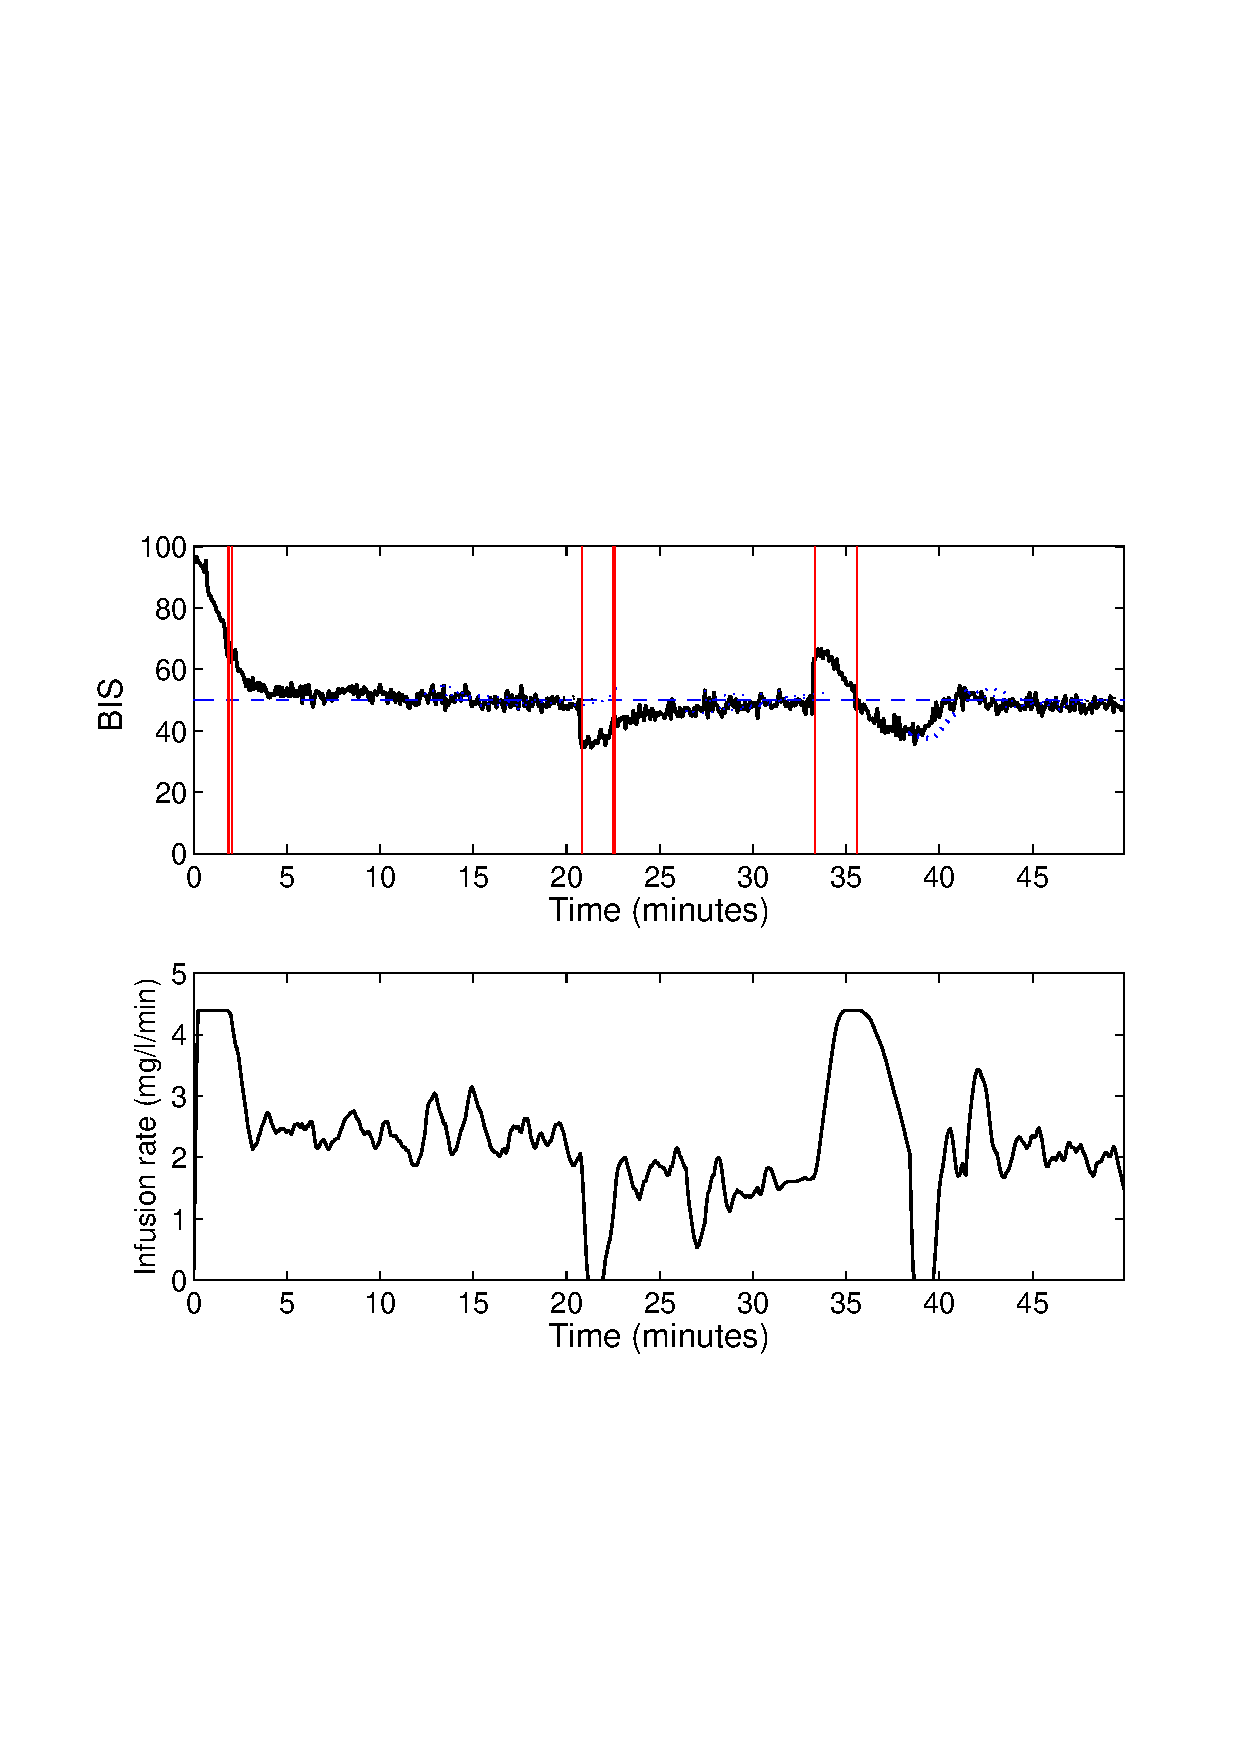
\includegraphics[width=0.40\textwidth]{./articles/pics/aclac_paper/fig2ColsedLoopContrlSim.pdf}%, height=0.45\textwidth
%\caption{Closed-loop control simulation of patient BIS using adaptive predictive control with change detection algorithm. Disturbances appears at $t=20.8 min$ and $t=33.3 min$. Upper figure show BIS evolution (solid line), BIS target (dashed line) and model predictions (dotted line). Vertical lines indicates a change detection. Lower figure presents infusion rate.}
\caption{ACLAC simulation result. Disturbances appears at $t = 20.8$ min and $t = 33.3$ min. The upper figure shows BIS evolution (solid line), BIS target (dashed line) and model predictions (dotted line). Vertical lines indicate detected change points. The lower figure presents the infusion rate.}
\label{fig:fig2ColsedLoopContrlSim}
\end{figure}

Figure~\ref{fig:fig1Comparison} shows a comparison of the proposed
ACLAC performance is done with a similar algorithm without change
detection. Change detection is shown with vertical lines. We can see
that if there are no disturbance both approaches show identical
performance. However, after the disturbance affects the patient, ACLAC
(solid line) performs better than a similar controller without an
explicit change detection mechanism. The disturbance rejection is
quite effective with ACLAC. Observe that the algorithm without change
detection is not able to take the patient quickly to the target due to
the use of a less accurate model.

\begin{figure}[htb!]
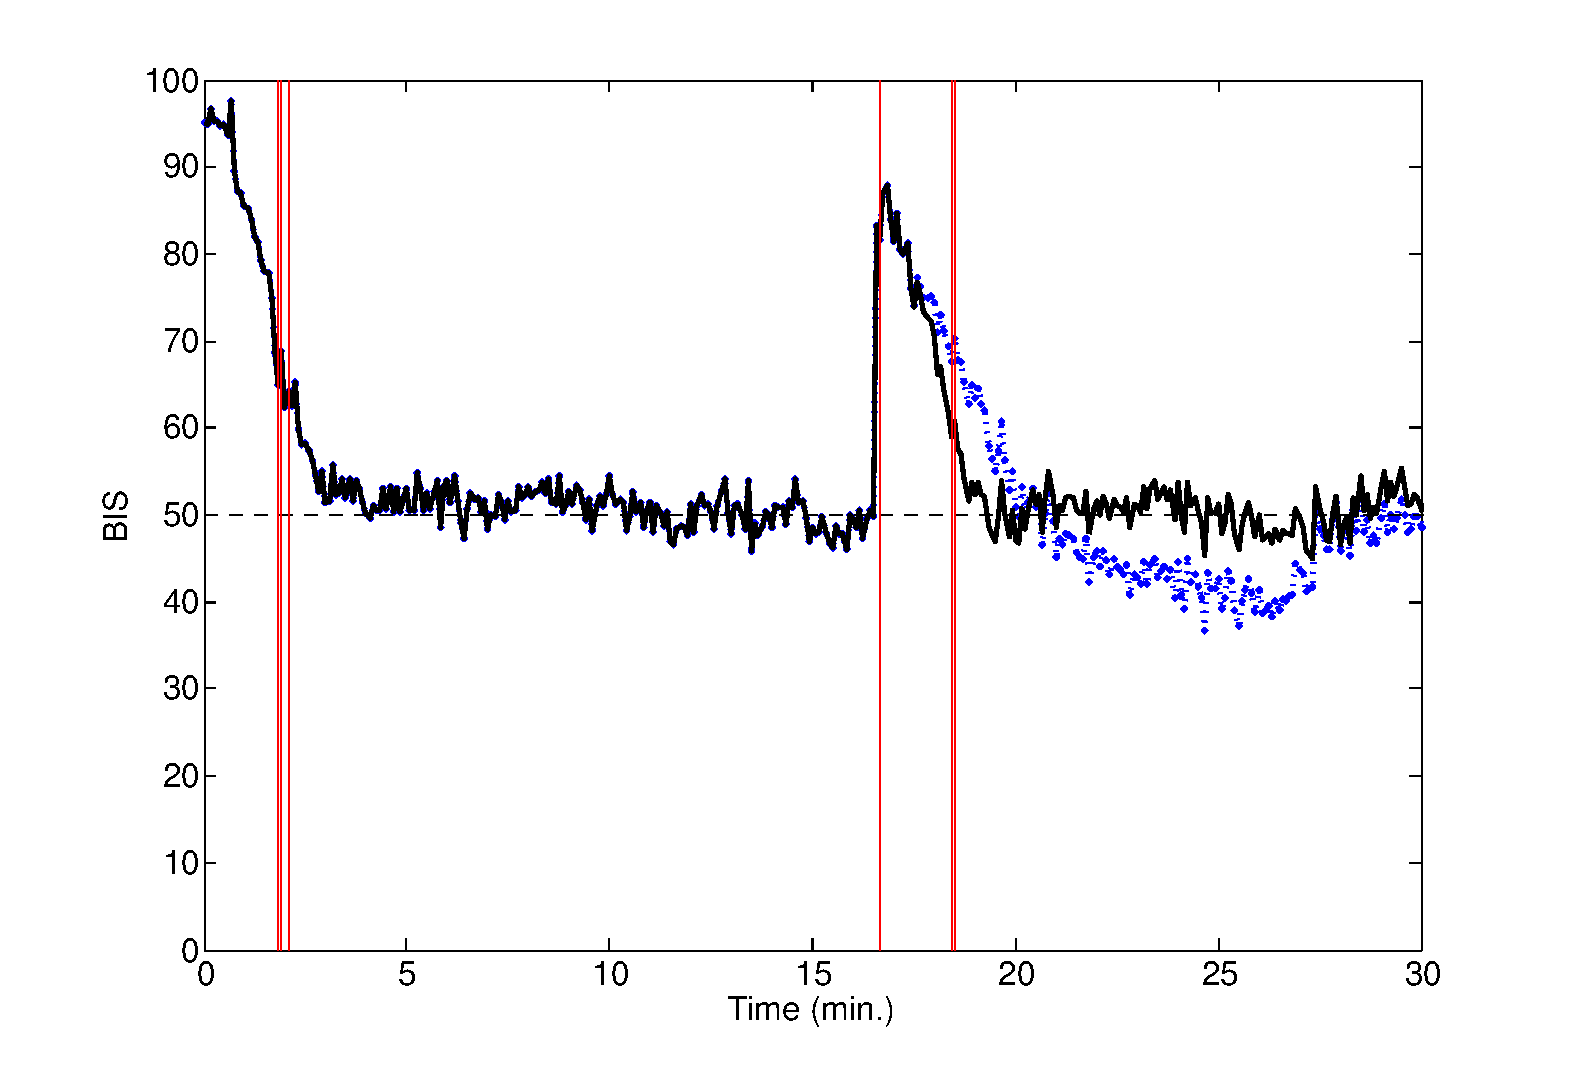
\includegraphics[width=0.45\textwidth]{./articles/pics/aclac_paper/fig1Comparison.pdf}%, height=0.3\textwidth
\caption{Comparison of ACLAC (solid line) and predictive controller
  using a fixed time window for identification (dotted line) instead
  of relying on explicit change detection.}
\label{fig:fig1Comparison}
\end{figure}

\section{Conclusion and future work}
Close-loop control of hypnosis for patients undergoing general
anesthesia is an important problem that is challenging because of the
inter- and intra-patient variability in response behavior.  We
proposed ACLAC - an adaptive scheme of the controller that uses
explicit change detection mechanism for quicker adaptation to the
changes in patients response.

We performed experimental evaluation of the change detection mechanism
on real data collected from the patients and of ACLAC as a whole in
the simulation.  The results indicate that introduced explicit change
detection mechanism indeed improves the performance of ACLAC in
comparison with analogous adaptive schemes based on fixed time window
instead of detecting changes.

In our future work we plan to (1)~perform more extensive evaluation of
the considered change detection method with other relevant approaches
including e.g. PHT-FM~\cite{GamaRealTimeAlg}, CUSUM~\cite{Cusum}, ADWIN~\cite{adwin07} and Quantile Index~\cite{Maslov_QI} on a larger set of BIS signals, and 
(2)~validating the proposed closed-loop hypnosis control approach in
the real operational settings, i.e. in a surgery room.
%
%Our approach is unsupervised but also have limitations which are described above.
%
%We believe that the best approach is to use ensemble method which incorporates strong points from other methods.
%
%In a future work we want to modify proposed approach to more consistent for on-line sequential processing and change detection.
% We want to modify optimal partitioning method for on-line usage and
% use it in ensemble with sequential on-line change detection methods
% (PHT-FM, CUSUM, etc.).

%\section{Acknowledgements}
\paragraph{Acknowledgements.}
This work is under the auspicious of the research Project
DPI2010-18278 supported by ``Ministerio de Ciencia e Innovación" of the
Spanish Government.

%~\cite{GamaRealTimeAlg}
%~\cite{GamaDecisionSupportSystems}

%\bibliographystyle{latex8}
%\bibliographystyle{abbrv}
\bibliography{references_aclac}



\chapter{Article: BLPA}
BLPA: Bayesian Learn-Predict-Adjust Method for Online  Detection of Recurrent Changepoints.

\begin{abstract}
Online changepoint detection is an important task for machine learning in changing environments.
Presence of noise that can be mistaken for real changes makes it difficult to develop an effective approach that would have a low false alarm rate and being able to detect all the changes with a minimal delay.
In this paper we study how performance of popular Bayesian online detectors can be improved in case of recurrent changes. Modeling recurrence allows us to anticipate future changepoints and predict their time locations.
We propose BLPA, an efficient approach for inducing and integrating recurrence information in the streaming settings, and demonstrate its effectiveness in the experimental study on synthetic and real-world datasets.
\end{abstract}

\section{Introduction}
Online change detection is practically relevant in many domains, such as medicine, energy production, industrial processes monitoring~\cite{Nikiforov}.
In machine learning and data mining research areas change detection is often studied in the context of problem of concept drift happening due to changes in the underlying data distribution over time~\cite{Widmer96}. A popular approach for handling concept drift is to monitor data or model performance for changes and to adapt model using most recent data collected after the last detected change~\cite{GamaACMCS2014}.
%It is easier to make decisions once you are aware about the changes in a current situation.
%For a self-driving car it is important to be aware about the changes in a road condition to avoid accidents.
%If you are a user of a mobile devise equipped with a set of sensors
%changes detected in the generated data may be used to issue a recommendations to improve your health conditions or to improve your performance in a sport activity.

In this paper we consider a change detection task in a one-dimensional univariate time series data streams.
Further in the text we denote a univariate vector of observations either as $\langle x_i \rangle_{i=1}^n$ or as $\pmb{x}_{1:n}$, i.e.
\[
\pmb{x}_{1:n} \equiv \langle x_i \rangle_{i=1}^n \equiv \langle x_1, \dots, x_n \rangle
\]
Input to the change detector is a vector of observations
$\langle x_t \rangle$ indexed by the timestamps $t \in \T$.
Timestamps is an ordered vector of time moments $\T \equiv \langle t_1, \dots, t_T \rangle$ when observations were taken with a constant sampling rate.
\textit{Changepoint is a time moment when statistical properties of the data stream change significantly according to the predefined criteria.}
Changepoint is identified by the moment of time when it happened (further - `time location of the change').
%~\footnote{Further in the text the time when change has occurred is also called `time location of the change'.}.
The sequence of changes is denoted as $\Collect{c_i}_{i=1}^k \in \T$ and an individual change from this sequence as $c_i$.
Changes should be detected online when the only information observed until current moment of time can be used for an analysis.

%\subsection{Change detection problem}\label{sec:change_detection_problem}
The top plot (A) in the Fig.~\ref{fig:trellis_struct} illustrates an example of the input signal with three changepoints in the mean value at the moments $\pmb{c}_{1:3}=\langle 5, 10, 14 \rangle$.
Change is usually detected with some time delay $\delta$.
The change detection task is to detect changes $\pmb{c}_{1:3}$ with as small a possible delay $\delta$  while not alarming changes at any other time moments, i.e.\ avoiding false alarms as much as possible.
%The changepoint detection problem is illustrated in Fig.~\ref{fig:trellis_struct}.
%The top plot (A) illustrates the input signal $\pmb{x}_{1:t}$.
%There are three changepoints in the mean value at the moments $\langle 5, 10, 14 \rangle$.
%The change detection task is to detect these changes with as small a possible time delay while not alarming changes at any other time moments.
%
%\subsection{Performance of the change detector}
%Change detector can be viewed as a binary classifier assigning classes `change'/`not change' to the incoming observations $x_t$.

An event when the change was alarmed by the detector while there is actually no change is called False Positive (FP).
% (e.g. alarm is caused by the noise or by outliers)
Outliers and noisy changes in the input signal may cause FPs. % events what in turn may lead to the wrong decision costing a lot.
%Change detector can be viewed as a binary classifier
%whose output for each input observation $x_t$ is the label $\lbl{+}$ if change is alarmed and denote it $\Event{t}{+}$, and label $\lbl{-}$ otherwise, which we denote as  $\Event{t}{-}$.
% %, which we call a \textbf{change detection event (CDE)}
%
%Let  denote the label assigned at the moment $t$ as $\Event{t}{+}$ if it was a change and $\Event{t}{-}$ otherwise.
%Change detector can be viewed as a binary classifier
%assigning to each input observation $x_t$
%label $\lbl{+}$ at time moment $\Event{t}{+}$ if change is alarmed
%and label $\lbl{-}$ at corresponding  time moment $\Event{t}{-}$ otherwise.
%To assess detectors' performance we define True Positive (TP),
%False Positives (FP), True Negatives (TN) and False Negatives
%(FN) events as follows:
%
%\subsection{Problem formulation}
% === START \subsection{Prblem formulation}
%Change detector may be considered as a binary classifier assigning labels change/not change to the incoming observations.
%Successful detection of the change is then counted as a True Positive (TP).

While the majority of existing change detection techniques focus on individual changepoint detection and assume that changepoints are not predictable, Fig.~\ref{fig:trellis_struct} illustrates use cases in which changes are expected to reappear over time.
In this paper we focus on such setting, addressing the problem of detecting changes in noisy signals with recurrent changes.

%More formally the problem is formulated as follows:~\textbf{reduce FP rate of the change detector as much as possible while not skipping actual changepoints.}
%keeping TP rate as high as possible
Our approach (called \textbf{BLPA} method) is based on the hypothesis that if probability distribution of the time intervals between changepoints differs from the probability distribution of time intervals between outliers we can use this information to predict time locations of the changes and skip outliers and therefore achieve better TP/FP rates.

%\subsection{Bayesian detector and BLPA method}
BLPA is a new online detection method. It extends the Bayesian Online Changepoint Detector (\textbf{BD}) proposed in~\cite{mackay2007} by embedding into it a Predictive Change Confidence Function (\textbf{PCCF}), which we introduced recently in~\cite{MaslovSDM2016}, in order to predict future changepoints in the input data stream, adjust detector's settings dynamically and to reduce FP rate.
% $\langle c_1, \dots, c_k \rangle$
%of observations $\langle x_1, \dots, x_t \rangle$

In short, BD detector works by recursively estimating posterior probability distribution $P(r_t | \pmb{x}_{1:t}, \theta)$ of the \textit{run length}  variable $r_t$ which is a time since the last changepoint.
Changepoint is an event when
\[
    \operatorname*{arg\,max}_{r_t} P(r_t | \pmb{x}_{1:t}, \theta) = 0
\]
%$r_t = 0$
The \textit{posterior} distribution is recalculated then every time a new measurement $x_t$ is observed using Bayes` theorem to update parameters of the distributions used to model data
%\[
%P(r_t | \pmb{x}_{1:t}) = \frac{P(r_t, \pmb{x}_{1:t})}{P(\pmb{x}_{1:t})}
%\]
and the law of total probability
%$P(x) = \sum_{y} P(x|y) p(y)$
\[
P(r_t|\:\LargeCdot) = \sum_{r_{t-1}} P(r_{t} | \: r_{t-1},\:\LargeCdot) \: P(r_{t-1}|\:\LargeCdot)
\]
to consider all possible run's values in the past.
% and weight them by their conditional on observed data probabilities.
%In BD detector time locations of the changepoints are modelled using a \textit{run length} variable $r_t$ which is a time since the last changepoint.
% START Move to the detector description?
% The plot (B) in Fig.~\ref{fig:trellis_struct} illustrates run length values for the signal on the top plot (A).
% END Move to the detector description?
%Changepoint at time $t$ then corresponds to the zero value of the run length $r_t \equiv 0$.
%
%In BD detector changes are detected by estimating the posterior probability distribution of the run lengths
%$P(r_t | \pmb{x}_{1:t} )$
%$P(r_t | \langle x_i \rangle, \theta )$
%at every time step $t$ after a new observation $x_t$ is observed.

%we embed PCCF into the BD on the step when
The \textit{prior} probability of the change $P(r_t=0|t)$ in BD detector is specified using the constant-value hazard rate $h$ which is an instant prior probability to observe a change and which is supposed to be known before the change detection process starts.
% past using the sum rule of statistics $P(x) = \sum_{y} P(x|y) p(y)$.
The uniform \textit{non-informative} prior does not hold enough information to distinguish outliers and noisy changes from the changepoints.
%
We improve performance of the BD detector by using an \textit{informative} prior distribution in a form of the PCCF function which parameters are the average time interval $\mu$ between consecutive changepoints $\langle c_i - c_{i-1} \rangle$ and standard deviation $\sigma$.
% to be able to estimate the relative probability to observe change versus outlier at the given time moment.
%This approach is applied to the case of recurrent changepoints which occur after approximately equal time intervals.
Given current estimate of $\mu$ and $\sigma$ PCCF gives a prior probability $\mathcal{P}(t | \mu,\sigma)$ to observe recurrent changepoint at time $t$.
%Time intervals between recurrent changepoints are modelled using a Gaussian distribution $N(\mu,\sigma)$.
% where $(\mu,\sigma) \sim F(\cdot | \theta)$.
% inferred from the stream of detected changepoints $\langle c_j \rangle$.
During the change detection process parameters of the BD detector are adjusted dynamically according the predictions in order to skip possible noisy changes in between changepoints.
When a new changepoint is detected  (or its location is provided by outer source) parameters $(\mu, \sigma)$ are updated using Bayesian rule and new prediction
$\mathcal{P}(t | \mu_{\text{new}}, \sigma_{\text{new}})$ is made.
%$\mathcal{P}(t | \: \langle c_j \rangle), \forall c_j < t$
%
%\subsection{Contribution}
% Our contribution can be summarized as follows.
%Most of the existing change detection methods are \textit{re}active meaning that detector's output might be refined by post-processing of the collected data to localize changepoints more accurately.
%%
%-FIX BD detector in its original version~\cite{mackay2007} works by sequentially updating prior probability estimates to posterior using Bayesian statistics rules.
%%
%By extending BD with PCCF we make the detector \textit{pro}active - we predict time locations of the future changes and adjust detector's settings dynamically according to the estimated probabilities of the changes.

%\subsection{Content outline}
The paper is organized as follows.
In Section~\ref{sec:related_work} we review related works.
In Section~\ref{sec:bd_detector} we describe in detail how the Bayesian Change Detector proposed in~\cite{mackay2007} works.
In Section~\ref{sec:pccf} we describe \textbf{PCCF} function used to predict recurrent changes.
In Section~\ref{sec:data_model} we describe the data model common for the  input signal of observations
%$\pmb{x_{1:T}}$
$\langle x_i \rangle$
and for the time intervals between changepoints
%$\pmb{c_{1:k}}$
$\langle c_i - c_{i-1} \rangle$.
%
In the Section~\ref{sec:BLPA} we describe the \textbf{BLPA} algorithm which is a \textbf{BD} detector integrated with the \textbf{PCCF} function.
%
In the Section~\ref{sec:experiments} we describe experimental results demonstrating improved performance of the \textbf{BD} detector when integrated with the \textbf{PCCF}.
%
%Further we will use the next abbreviations.
%\begin{itemize}
%    \item \BD - `Bayesian Online Changepoint Detector'~\cite{mackay2007}
%    \item \PCCF - Predictive Confidence Change Function~\cite{MaslovSDM2016}
%    \item \BLPA - Learn-Predict-Adjust change detector
%\end{itemize}
%
%\PCCF parameters are expected time interval between consecutive
%changes $\mu^C$ and standard deviation of these time intervals
%$\sigma^C$.
%
% First we estimate parameters from historical data.
%
% After that we predict time locations of the future changes using \PCCF function.
%
% When the new changepoint is detected we update $\mu^c$ and $\sigma^C$ using Bayesian rule.
% Once the changepoint is detected the probability distribution
% parameters are updated and a new prediction is made.
%In this work we propose a novel Learn-Predict-Adjust method (BLPA) based on
% In \BD data is assumed to be Gaussian with the unknown mean and
% variance.
%
%Prior for the mean value and precision $\tau = 1/\sigma$ is given
%by inverse-normal gamma distribtuin.
%
%The same model we assume for the time intervals between
%changepoints.
%Update procedure is also the same.
%
%\PCCF models changepoints using Gaussian distribution with
%parameters $(\mu^C, \tau^C)$.  So it is a second layer.
% PCCF's parameters are learned and updated online using the same
% data model which is used in the \BD detector to model the input
% data.
%
% Two-layers: 1) detect changes in the input data 2) once change in
% detected - update model for the changepoints and make a new
% prediction.
%
% \BLPA method includes the \BD detector proposed
% in~\cite{mackay2007} and \PCCF function which we developed in our
% previous work~\cite{MaslovSDM2016}.

%------ RELATED WORK START %
\section{Related work}
\label{sec:related_work}

While many change detection methods have been developed~\cite{Nikiforov,Polunchenko2011} for offline and online settings, they typically assume that changes occur at random in time, and are independent from each other.
In practice, however, in many industrial applications changes occur with some regularity (e.g.\ seasonality).
Our BLPA approach captures this information from data, and utilizes it for improving the accuracy of a Bayesian online change detection.

%The close approach to ours is
In the Bayesian online change detector proposed in~\cite{mackay2007} and extended in~\cite{Wilson2010a} authors model time intervals between change points (run lengths) using the hazard rate.
This approach allows to take into account recurrence by tuning single parameter, but it does not allow to distinguish outliers from changes which may appear between them.
In~\cite{huang2014detecting} data stream volatility, defined as the rate of detected changes, is used to make detector more reactive.
%, which is aimed at capturing episodic reoccurrences, as opposed to modeling reoccurrences in the long run.
We concentrate on the problem of improving change detection by predicting time locations of the changes in the future in order to better distinguish outliers from real changes.

In BD~\cite{mackay2007} the hazard rate is a constant value assumed to be known in advance.
%
This is not a realistic assumption and this problem has been addressed in~\cite{WilsonBayesOnline} where authors proposed an on-line inference
procedure to estimate $h$ parameter for the case if hazard rate is unknown and can itself undergo changes while new data
arrives.
%proposed an online inference algorithm to learn and reestimate $h$ value Online while observing a new data.
%
% In~\cite{WilsonBayesOnline} authors proposed an on-line inference procedure to estimate $h$ parameter for the case if hazard rate is unknown and can itself undergo changes while a new data arrive.
In~\cite{DowneyChp} authors proposed an algorithm 
%based on Bayesian statistics and this algorithm 
which can detect and locate changepoints simultaneously using Bayesian statistics approach.
%, and also predict the distribution of the next changepoint.
%
In~\cite{saatcci2010gaussian} authors use Gaussian Process model to compute predictive distribution $p(x_{\textbf{new}} | \pmb{x}_{\textbf{old}})$.

Our method is different from these ones because we combine change detection and prediction tasks. 
We add a second layer (PCCF function) on top of the change detection algorithm allowing to predict future recurrent changes and adjust detectors settings dynamically.
This second layer is a change detector itself in the sense that it automatically incorporates changes in underlying distribution of the time intervals between recurrent changes.
%Particularly we combine an Online Bayesian change detector and the prediction confidence change function. 
%previous work considered only one aspect in the problem of changepoint detection, either change detection algorithm itself or *something to describe this*.
%In this paper, 
%In this two-layer framework, model will be updated once changes are detected which will lead to better performance.

In our previous work~\cite{MaslovSDM2016} we demonstrated how to integrate PCCF with the very naive threshold based detector in a heuristic way. 
The BLPA method we propose here is a more advanced.
% and more sound technique.
It integrates PCCF natively into the BD detector using Bayesian statistics framework.
BLPA updates both parameters of BD and PCCF sequentially, detects changes, predicts future changes and adjusts parameters of the BD detector according to the predictions in order to skip noisy changes and outliers while detecting changes of interest.
% In~\cite{WilsonBayesOnline} author proposed an on-line inference procedure to
% estimate $h$ parameter for the case if hazard rate is unknown and can itself
% undergo changes while a new data arrive.
% In~\cite{DowneyChp}

A few other and more remote lines of work relate to our approach via attention to recurrent concept drift~\cite{GamaK11,DBLP:journals/tnn/GomesGSR14,DBLP:journals/ida/GomesSR12}, predictability of concept drift~\cite{Ang2013}, or change detection with delayed labeling~\cite{DBLP:conf/icdm/Zliobaite10}.
These approaches are specific to handling concept drift, while our focus is on generic online change detection and its accuracy.


\section{Online Bayesian Change Detector (BD)}
\label{sec:bd_detector}
In this section we describe the Bayesian Online Changepoint Detector proposed in~\cite{mackay2007}.
As we mentioned - to model time occurrences of the changes authors introduce a latent variable run length $r_t$ which is the number of time steps since the most recent change.
%\textit{Run length $r_t$ is the number of time steps since the most recent change}.~\cite{mackay2007},~\cite{WilsonBayesOnline}.
In Fig.~\ref{fig:trellis_struct} plot \textbf{(A)} you can see an illustrating example of the input signal and corresponding run values on plot (B).

On each time step there are two possibilities: either the run length increases $r_t = r_{t-1}+1$ or changepoint occurs $r_t = 0$.
The conditional prior $P(r_t | r_{t-1})$ of the change is given by a constant-value hazard rate $h$ (Equation~\ref{eq:hazard_rate}).
%..Hazard rate $h$ is the instantaneous probability to observe of an event given that it has not happened yet.
\begin{equation}
    p(r_t | r_{t-1}) =
    \begin{cases}
    1 - h \text{\:\:\: if }  r_t = r_{t-1} + 1 \\
    h \text{\:\:\:\:\:\:\:\:\:\:\:  if } r_t = 0
    \end{cases}
    \label{eq:hazard_rate}
\end{equation}
% ??
The plot \textbf{(C)} in Fig.~\ref{fig:trellis_struct} illustrates the
message-passing algorithm to compute prior probabilities of the
changepoint at any time moment given the boundary condition
$P(r_1=0)=1.0$ that change occurred at the moment $t=1$.
%
Each node (circle) represents a hypothesis about the current run length value.
%
From each node there is a solid line upwards depicting probability of increasing of the run on the next time step (no change) and a dashed line going downwards depicting probability of the change.

At each time step the probability of the changepoint is estimated by calculating posterior probability distribution of the run length value given the data so far observed (Equation~\ref{eq:r_t_posterior}).
\begin{equation}
    P(r_t | \pmb{x}_{1:t}) = \frac{P(r_t, \pmb{x}_{1:t})}{P(\pmb{x}_{1:t})}
    \label{eq:r_t_posterior}
\end{equation}
% % The marginal predictive distribution $P(r_t, x_{1:t}) \sim \sum_{r_{t-1}} P(r_t, r_{t-1}, x_{1:t}) $
% % $\sim \sum_{r_{t-1}} P(r_t, r_{t-1}, x_{1:t}) $
% % $P(r_t | x_{1:t}) = \frac{P(r_t, x_{1:t})}{P(x_{1:t})}$. \\
The joint probability of the run length values and observed so far data
can be sequentially computed using recursive procedure in Equation~\ref{eq:bd_recursive_formula} as it is described in~\cite{mackay2007}:
\begin{multline}
    P(r_t, x_{1:t}) = \sum_{r_{t-1}} P(r_t, r_{t-1}, x_{1:t}) = \\
    \sum_{r_{t-1}} P(r_t, x_t \: | \: r_{t-1}, x_{1: t-1}) \: P(r_{t-1}, x_{1:t-1}) = \\
    \sum_{r_{t-1}} P(r_t | r_{t-1}) P(x_t | r_{t-1}, x_t^{(r)}) P(r_{t-1}, x_{1:t-1})
    \label{eq:bd_recursive_formula}
\end{multline}
where $x_t^{(r)} \equiv \langle x_{t-r+1},\dots,x_t \rangle$ is input data sub-interval associated with the run length $r$.
%
%From Equation~\ref{eq:bd_recursive_formula} it can be seen that we also need to calculate a marginal predictive distribution of the new observation $x_t$ which can be calculated by
Marginal predictive distribution of the new observation $x_t$ is computed using the sum rule:
\begin{equation}
    P(x_{t} | \pmb{x}_{1:t-1}) = \sum_{r_t} P(x_{t}|r_{t}, \pmb{x}_t^{(r)}) P(r_t | \pmb{x}_{1:t-1})
    \label{eq:bd_marginal_predictive}
\end{equation}
% \textit{(calculated like in~\cite{JordanChapter9} 9.1.2)}.
%
\begin{figure}[htb!]
    \includestandalone[width=0.40\textwidth]{images/blpa_article/trellis-struct}
    \caption{
        The changepoint detection problem.
        (A): Input signal.
        (B): A particular realization of the run length path corresponding to the actual changepoints locations in the input signal.
        (C): Directed graph representing all possible run length paths.
        \textit{The figure is replicated from the illustration in~\cite{mackay2007}.}
        }
\label{fig:trellis_struct}
\end{figure}
%
% https://en.wikipedia.org/wiki/Normal-gamma_distribution
% Marginal distribution (predictive) over $x$ is a three-parameter non-standardized Student's t-distribution.
% is non-standardized Student's t-distribution
%\begin{equation}
% p(x | \nu, \mu, \sigma) = \frac{ \Gamma (\frac{\nu+1}{2}) } { \Gamma (\frac{\nu}{2}) \sqrt{\pi \nu} \sigma }
%\end{equation}
%% function p = studentpdf(x, mu, var, nu)
%%
%%  p = studentpdf(x, mu, var, nu)
%%  This form is taken from Kevin Murphy's lecture notes.
% c = exp(gammaln(nu/2 + 0.5) - gammaln(nu/2)) .* (nu.*pi.*var).^(-0.5);
% p = c .* (1 + (1./(nu.*var)).* (x-mu).^2).^(-(nu+1)/2);
%
%Plot (B) on Figure~\ref{fig:trellis_struct}) illustrates an example of the
%run length values for the example
%for the input signal (plot \textbf{(A)}
%on Figure~\ref{fig:trellis_struct}) are depicted on plot \textbf{(B}).

\section{PCCF function}
\label{sec:pccf}
% predictive confidence change function
In this section we show how to compute PCCF function used to predict time locations of the recurrent changes in the future.
%giving probability distribution of the future changepoints.
We consider a discrete case when observations are obtained at the
discrete time moments $\langle t \rangle_{t=1}^T$ with a constant sampling rate.
%
Probability distribution for the discrete sets is defined using
Probability mass function (\textbf{Pmf}).
As mentioned earlier we assume that changes \textit{re-}occur after
`approximately' equal time intervals.
To model time intervals between consecutive changes
$\langle c_i - c_{i-1} \rangle$
we use the Gaussian distribution assuming that standard deviation is small enough so that probability to observe the change $c_i$ before $c_{i-1}$ is extremely small.
\begin{definition}
    \label{def:recurrentdefinition}
    \textit{
        Changes $\Collect{c_i}_{i=1}^k$ are recurrent if
    }
    \begin{equation}
        p(c_{i+1} = t \: | \: \theta^C) = p(c_1 = t - c_{i} \: | \: \theta^C),
        \label{eq:procnorefs}
    \end{equation}
    \textit{
        where
        $\theta^C=(\mu^C,\sigma^C)$,
        $c_1$ is the time of the $1^{st}$ change,
        $c_i$ is the time of the $i^{th}$ change.
    }
\end{definition}
%
This definition corresponds to the generative model defined by
Equation~\ref{eq:recurrent_generative_model} in which every next
change $c_{i+1}$ happens after time intervals $\Delta$ which are
samples from the Gaussain distribution $N(\mu^C, \sigma^C)$.
\begin{equation}
    c_{i+1} = c_i + \Delta,~~\text{where } \Delta \sim N(\mu^c, \sigma^c)
    \label{eq:recurrent_generative_model}
\end{equation}
%
To predict future changes we introduce the notion of the
Predictive Change Confidence Function (\PCCF)~\cite{MaslovSDM2016}.
\begin{definition}
    \label{def:pccf_definition}
    %== Initial definition
    % PCCF is the probability to observe any recurrent change out
    % of sequence of all possible changes $c \in \Collect{ c_i }_{i=1}^k$ at any given time moment $t$:
    %== End Initial definition
    \textit{
        \PCCF is a \textbf{Pmf} defined on a discrete set of time moments
        $\langle t \rangle_{t=1}^T$ giving a probability
        to observe recurrent change $\forall c \in \Collect{ c_i }_{i=1}^k$
        at the time moment $t$
    }
    \begin{equation}
        %\mathcal{P}(t\:|\:\theta^C)=\sum_{i=1}^{k} p(c_i = t \: | \: \theta^c)
        \mathcal{P}(c=t|\mu^c,\sigma^c)=\sum_{i=1}^{k} p(c_i=t|\mu^c,\sigma^c)
    \end{equation}
    \textit{
        where $p(c_i=t|\mu^c,\sigma^c)$ is a \textbf{Pmf} for an
        individual change $c_i$.
    }
    %,~\theta^c = (\mu^c, \sigma^c) % where $\theta^c = (\mu^c, \sigma^c)$.
\end{definition}
% NO (?) Further $h(t) \equiv \mathcal{P}(t\:|\:\theta^C)$
%
It is important to note that \textit{change-}events $\langle c_i \rangle$ are
independent.
%
Every $c_i$ can happen at any moment of time according to its
individual \textbf{Pmf} $p(c_i=t|\mu^c,\sigma^c)$.
%
%According to the Definition~\ref{def:recurrentdefinition}
%\textbf{Pmf} of the change $c_{i+1}$ is conditioned on the time
%of the $i^{th}$ change $c_i$.
%
Following the sum rule for total probability\footnote{$P(x) = \sum_{y} P(x|y) p(y)$} in order to compute Pmf of $c_{i+1}$ we need to consider all
possible time locations of $c_i$.
\begin{equation}
    p(c_{i+1} = t) = \sum_{\tau = i}^{t-1} p(c_{i+1}=t \: | \: c_i = \tau) p(c_i = \tau).
    \label{eq:sum_rule_recurrent}
\end{equation}
According to the definition~\ref{def:pccf_definition} PCCF is a sum of individual \textbf{Pmf}'s of the changes which might happen till current moment of time
\begin{eqnarray}
    \notag
    \mathcal{P}(t) & = &  \sum_{i=1}^{t} \sum_{\tau = i}^{t-1} p(c_{i+1} = t | c_{i} = \tau)  p(c_{i} = \tau) \\
    & = & \sum_{i=1}^{t} \sum_{\tau = i}^{t-1}
    p(c_{1} = t - c_{i})  p(c_{i} = \tau).
    \label{eq:pccf}
\end{eqnarray}
% \subsection{The exact PCCF for Gaussian distribution.}
%% Start Old version
% In the considered case of the Gaussain distribution $p(x|\mu^c,\sigma^c) \sim 0$ for all $x \leq 0$
% Equation~\ref{eq:sum_rule_recurrent} is a convolution of the
% \textbf{Pmf} $p(c_1)$ of the $1^{st}$ recurrent change, which is
% given as a boundary condition, and of the Pmf of the change $c_i$
% calculated in the previous step:
%% End Old version
Right side of the Equation~\ref{eq:sum_rule_recurrent} is a convolution for the Pmf $p(c_1)$ of the $1^{st}$ recurrent change and of the Pmf of the change $c_i$ computed in the previous step
\begin{eqnarray} \notag
    p(c_{i+1}) & = & (p(c_1) \ast p(c_i)) [\tau] \\
    & = & \sum_{\tau = 1}^{t-1} p(c_1 = t - \tau) p(c_i = \tau).
    \label{eq:sum_rule_convolution}
\end{eqnarray}
%
The convolution of two Gaussian distributions is also Gaussian distribution
\begin{equation}
    (p(x|\mu_1, \sigma_1) \ast p(x|\mu_2, \sigma_2)) = p(x| \mu_1 + \mu_2, \sqrt{\sigma_1^2 + \sigma_2^2}).
\end{equation}
%Using this observation
PCCF (Eq.~\ref{eq:pccf})
can be written as a t-fold convolution
%and computed analytically
\begin{equation}
\mathcal{P}(t) =
(
\underbrace{
    p(c_1) \ast p(c_1) \ast \dots  \ast p(c_1)
}_\text{t}
)
\end{equation}
% https://en.wikipedia.org/wiki/Renewal_theory !!!
% http://mathworld.wolfram.com/NormalSumDistribution.html
% Charles M. Grinstead "Introduction of probability"
% http://www.dartmouth.edu/~chance/teaching_aids/books_articles/probability_book/book.html
% https://www.dartmouth.edu/~chance/teaching_aids/books_articles/probability_book/Chapter7.pdf
%??Uncomment? = p(c_1)^{\ast t}.
%
%
%Therefore PCCF for the moment $t$ is a sum
which is equivalent to the sum
\begin{equation}
    \mathcal{P}(t) = \sum_{l=1}^{t} \frac{1}{\sigma \sqrt{2 \pi l}} \exp \left(\frac{-(t - l \mu)^2}{2 l \sigma^2} \right)
    \label{eq:gaussian_pccf}.
\end{equation}
The sum~\ref{eq:gaussian_pccf} describes renewal-reward process~\cite{cox1962renewal},~\cite{feller1968introduction}.
Using the renewal theorem~\cite{cox1962renewal}
%(Chapter 13~\cite{feller1968introduction}
we can calculate the limit of $\mathcal{P}(t)$ when $t \to \infty$
%given by expression~\ref{eq:gaussian_pccf_limit}
\begin{equation}
L = \lim_{t \to \infty} \sum_{l=1}^{\infty} \frac{1}{\sigma \sqrt{2 \pi l}} \exp\left(-\frac{(t- \mu l)^2}{2 l \sigma^2} \right) = \frac{1}{\mu}.
\label{eq:gaussian_pccf_limit}
\end{equation}
From Equation~\ref{eq:gaussian_pccf_limit} follows that PCCF converges to the constant value uniform distribution for large $t$ values.
%%%%%%%%%%% START COMMENT LIMIT CALCULATIONS
% We can replace $l$ by $t/\mu$ in the denominators since we are interested in the terms for which $l \sim t / \mu$ and when $t \to \infty$, $\lim_{t \to \infty}\left( \frac{1}{t} - \frac{1}{t/\mu} \right)=0$, we are making approximation error of order $(1 + o(1))$,
% \begin{equation}
%   L = \lim_{t\to\infty} \sum_{l=1}^{\infty} \frac{\sqrt{\mu}}{\sigma\sqrt{2\pi t}} \exp\left(-\frac{\mu^3 (t/\mu- l)^2}{2t\sigma^2}\right).
%   \label{eq:pccf_sum_decomposed}
% \end{equation}
% Exponential terms corresponding to $l$, for which $|t/\mu - l| \gg \sqrt{t}$, will have small values which we can ignored.
% Therefore, we need to estimate the sum consisting of the terms for $l \in [t/\mu \pm \sqrt{t}]$.
% It is convenient to consider a wider interval of width $t^{3/5} > \sqrt{t}$.
% Let us consider three intervals for $l$
% (1) $[0, t/ \mu - t^{3/5})$,
% (2) $[t/ \mu - t^{3/5}, t/ \mu + t^{3/5}]$,
% (3) $(t/ \mu + t^{3/5}, \infty)$.
% The components in the sum in Eq.~\ref{eq:pccf_sum_decomposed} are very small within the intervals (1) and (3) since both are bounded by $\exp(-\frac{\mu^2}{2 \sigma^2} N^{1/5})$.
% Therefore, we can find the limit by estimating the sum only within the interval (2):
% \begin{equation}
%   L = \lim_{t\to\infty} \frac{\sqrt{\mu}}{\sigma \sqrt{2\pi t}} \sum_{l=-t^{3/5}}^{t^{3/5}} \exp\left(-\frac{\mu^3 (t/\mu - l)^2}{2t\sigma^2}\right).
%   \label{eq:sum_before_integral}
% \end{equation}
% \Eq{eq:sum_before_integral} is the Riemann sum for the Gaussian integral $\int_{-\infty}^{\infty} e^{-a x^2} dx = \sqrt{\frac{\pi}{a}} $, thus
%%%%%%%%%%% END COMMENT LIMIT CALCULATIONS
%%% ?????????????????? START UNCOMMENT ???
%\noindent
%In~\cite{MaslovSDM2016} we prove that
%\begin{equation}
%%%L = \frac{\sqrt{\mu}}{\sigma \sqrt{2\pi}} \int_{-\infty}^{\infty} e^{-\frac{\mu^3 x^2}{2\sigma^2}} dx = \frac{1}{\mu}.
%L = \frac{1}{\mu^c}.
%\label{eq:pccf_limit_proof}
%\end{equation}
%%% ???????????????? END UNCOMMENT ???
Fig.~\ref{fig:pccf_example} illustrates two PCCF
functions (Equation~\ref{eq:gaussian_pccf}) with parameters $(\mu=10, \sigma=2)$ and $(\mu=15, \sigma=3)$.
\begin{figure}[htb!]
    \centering
    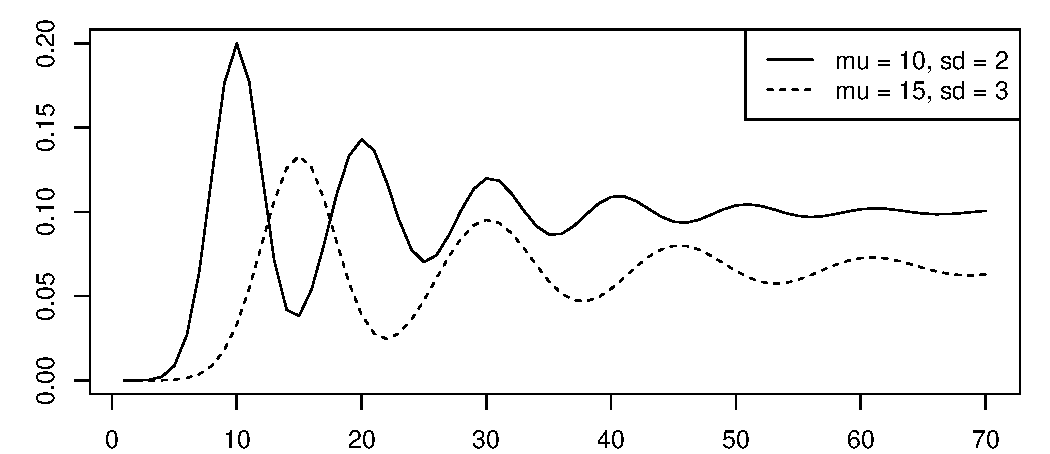
\includegraphics[width=0.40\textwidth]{images/blpa_article/pccfExamples.pdf}
    \caption{
        An example of two Gaussian PCCF functions.
        The limits are $\frac{1}{\mu^C}.$
    }
    \label{fig:pccf_example}
\end{figure}
% Local extrema of the PCCF function correspond to the time moments $l \mu, l \in \mathbb{Z}$.
% PCCF values converge to limits as defined in \Eq{eq:pccf_limit_proof} $L=1/10$ and $L=1/15$.
Prior and posteriors for the PCCF's parameters are estimated and updated using the procedure described in Section~\ref{sec:data_model} describing data model.

\section{Data model}
\label{sec:data_model}
%In~\cite{mackay2007} authors consider the general case of the Exponential family of distributions to model input data.
In this section we describe the data model which we use in BLPA.
% is the same both for input data stream of observations and for the stream of changepoints time locations.
%In BLPA method we use a particular set of probability distributions to model the data which we describe in this section.
There are two streams of data to be analysed.
The stream of input observations $\langle x_t \rangle$ and the stream of time intervals between changepoints  $\langle c_i - c_{i-1} \rangle$.
The first stream is used to detect changes and therefore to produce the second stream.
The stream of changes maybe updated by the outer sources providing additional information about time location of the changes.
E.g. there is a process running in parallel with the main detector which can run additional change-detection processes over collected data to identify locations of the changes in the past more precisely.
%
The stream of changepoints is used to predict future changepoints in order to adjust detector's settings to achieve a better performance.
% defined by the FA rate, detection delay $\delta$ and by TP rate.
%
Further, data $D$ is either input data stream of observations $\langle x_t \rangle$ or data stream of time intervals between consecutive changepoints $\langle c_i - c_{i-1} \rangle$.
In this section we describe a data model for $D$ common both for input signal and sequence of time intervals between changepoints.

Data $D$ is assumed to be generated by a Gaussian distribution with an unknown mean and variance.
We denote elements of $D$ by $\xcommon \in D$ with mean and variance $(\mucommon, \sigmacommon)$.

%\emph{I. Prior distributions.}\\
\subsection{Prior distributions.}
Following the notations in~\cite{JordanChapter9}, we use a \emph{normal-gamma} prior for $\mucommon$ and $\sigmacommon$:
%
\begin{align}
    %x_i &\sim N(\mu,\tau)~~i=1,...,n~\text{and}~\tau=1/\sigma^2\\
    \xcommon &\sim N(\mucommon,\taucommon),~~\taucommon=(1/\sigmacommon)^2\\
    \mucommon &\sim N(\muzerocommon,\kappazerocommon \taucommon)\\
    \taucommon &\sim Gamma(\alphazerocommon,\betazerocommon)
    \label{eq:theta_normal_gamma}
\end{align}
%
where $(\alphazerocommon, \betazerocommon, \muzerocommon,
\kappazerocommon)$ are hyperparameters.
%
The value $\taucommon$ is also named
\emph{precision}~\footnote{Further we use $\sigma$ and $\tau$
    parameters interchangeably.}.
%
The likelihood of data $D=\langle \xcommon \rangle$ is
%
\begin{equation}
P(D|\mucommon, \taucommon) = \Big(\frac{\taucommon}{2\pi} \Big)^{n/2}  \exp \Big (-\frac{\taucommon}{2}\sum_{i=1}^{n}(\xcommon-\mu)^2 \Big)
\end{equation}
%
The joint conjugate prior for parameters $(\mucommon,\taucommon
)$ is the defined \emph{normal-gamma} (\textit{NG}) distribution:
%
\begin{align}
    &P(\mucommon,\taucommon | \muzerocommon,\kappazerocommon,\alphazerocommon,\betazerocommon) =  N(\muzerocommon,\kappazerocommon \taucommon) Gamma(\alphazerocommon,\betazerocommon)\\
    &=\frac{1}{Z}\taucommon^{1/2}\exp\Big(-\frac{\kappazerocommon \taucommon}{2}(\mucommon-\muzerocommon)^2\Big)\taucommon^{\alphazerocommon-1}e^{-\taucommon \betazerocommon}\\
    &=\frac{1}{Z}\taucommon^{\alphazerocommon-1/2}\exp\Big(-\frac{\taucommon}{2}[\kappazerocommon(\mucommon-\muzerocommon)^2+2\betazerocommon]\Big)
\end{align}
%
where $Z=\frac{\Gamma(\alphazerocommon)}{\betazerocommon^{\alphazerocommon}}\Big(\frac{2\pi}{\kappazerocommon}\Big)^{1/2}$
is the normalized factor.

\subsection{Posterior distributions}
%Therefore,
The posterior can be derived as
%
\begin{align}
    P(\mucommon,\taucommon|D) &\varpropto P(\mucommon,\taucommon|\muzerocommon,\kappazerocommon,\alphazerocommon,\betazerocommon)P(D|\mucommon, \taucommon)\\
    &\propto N(\mucommon_n, \kappacommon_n \taucommon) Gamma(\alphazerocommon+n/2,\betacommon_n)
    \label{eq:mu_tau_posterior}
\end{align}
%
which is also a \emph{normal-gamma} distribution:
%
\begin{equation}
P(\mucommon,\taucommon|D)=NG(\mucommon,\taucommon|\mucommon_n,\kappacommon_n,\alphacommon_n,\betacommon_n)
\label{eq:mu_tau_prior}
\end{equation}
%
with the parameters
%
\begin{align}
    \mucommon_n&= \frac{\kappazerocommon}{\kappazerocommon + n} \muzerocommon + \frac{n}{\kappazerocommon + n} \bar x\\
    \kappacommon_n&= \kappazerocommon + n\\
    \alphacommon_n&= \alphazerocommon + n/2 \\
    \betacommon_n&= \betazerocommon+\frac{1}{2}\sum_{i=1}^{n}(\xcommon-\bar{x})^2+\frac{\kappazerocommon n(\bar{x}-\muzerocommon)^2}{2(\kappazerocommon+n)}
    \label{eq:update_rule}
\end{align}
%
%\begin{align}
%\mu_n&= \frac{\kappa_0}{\kappa_0 + n} \mu_0 + \frac{n}{\kappa_0 + n} \bar x\\
%\kappa_n&= \kappa_0 + n\\
%\alpha_n&= \alpha_0 + n/2 \\
%\beta_n&= \beta_0+\frac{1}{2}\sum_{i=1}^{n}(x_i-\bar{x})^2+\frac{\kappa_0 n(\bar{x}-\mu_0)^2}{2(\kappa_0+n)}
%\label{eq:update_rule}
%\end{align}
%
where $\bar{x}=\frac{1}{n}\sum_{i=1}^{n}\xcommon$ is the mean of sampled data.
% do we need this ?
The posterior distribution for $\taucommon$ is obtained by
integrating Equation~\ref{eq:mu_tau_prior} over $\mu$
(See~\cite{JordanChapter9}) --
%
\begin{multline}
    p(\taucommon | D, \muzerocommon, \kappazerocommon, \alphacommon, \betacommon) \varpropto\\
    Gamma(\alphacommon + n/2, \betacommon + \frac{1}{2} \sum_{i=1}^n (\xcommon-\bar{x})^2 +
    \frac{\kappacommon \kappazerocommon}{2(\kappacommon + \kappazerocommon)} (\bar{x} - \muzerocommon)^2 ))
    \label{eq:kappa_posterior}
\end{multline}
%
Given the updated parameters
$\theta=(\alpha_0, \beta_0, \mu_0, \kappa_0)$ using the rules~\ref{eq:update_rule} ,
the predictive distribution for a new data $x_{\text{new}}$ is
%
\begin{multline}
    p(x_{\text{new}} | \pmb{x}, \mu, \kappa, \alpha, \beta) = \\
    \int p(x_{\text{new}} | \mu, \tau) p(\tau | \pmb{x}, \mu_0, \kappa_0, \alpha, \beta) d \tau
    \label{eq:predictive_distribution}
\end{multline}
%
where
%
\begin{equation}
p(x_{\text{new}} | \mu, \tau) = (\frac{\tau}{2 \pi})^{1/2} e^{-\frac{\tau}{2} (x-\mu)^2} d \tau
\end{equation}
%
and $p(\tau | \pmb{x}, \mu_0, \kappa_0, \alpha, \beta)$ is given by~\ref{eq:kappa_posterior}.
%
Integral~\ref{eq:predictive_distribution} is a Pearson type VII distribution (Equation~\ref{eq:predictive_distribution2}) which is
equivalent of the non-standardized Student's t-distribution.
%~\cite{JordanChapter9}.
% https://en.wikipedia.org/wiki/Pearson_distribution#The_Pearson_type_VII_distribution
% The Pearson type VII distribution is equivalent to the non-standardized Student's t-distribution
\begin{equation}
p(x_{\text{new}})=\frac{1}{\alpha B(m - 1/2,1/2)} \Big (  1 + \Big (\frac{x_{n+1} - \lambda}{\alpha} \Big )^2 \Big )^{-m}
\label{eq:predictive_distribution2}
\end{equation}
%
where
%
\begin{align}
    m &= \alpha_0 + (n+1)/2\\
    %
    \alpha &= A \sqrt{ \sum_{i=1}^{n} x_i^2 + \kappa_0 \mu_0^2 - \frac{( \sum_{i=1}^{n} x_i + \mu_0 \kappa_0 )^2}{n + \kappa_0} + 2 \beta_0 }\\
    %
    A &= \sqrt{\frac{n+1+\kappa_0}{n+\kappa_0}}\\
    %
    \lambda &= \frac{\sum_{i=1}^n x_i + \mu_0 \kappa_0}{n + \kappa_0}
    \label{eq:posteriro_parameters}
\end{align}
%\alpha &= \sqrt{ \frac{n+1+\kappa_0}{n+\kappa_0} \Big ( \sum_{i=1}^{n} x_i^2 + \kappa_0 \mu_0^2 - \frac{( \sum_{i=1}^{n} x_i + \mu_0 \kappa_0 )^2}{n + \kappa_0} + 2 \beta_0 \Big)}\\
Predictive distribution~\ref{eq:bd_marginal_predictive} in case
of this data model is given by Equation~\ref{eq:predictive_distribution2}.
Please see detailed calculations in the Appendix.

\section{BLPA change detector}
\label{sec:BLPA}
% Explained in the Introduction: ?
The BLPA method is a combination of BD detector and PCCF predictive function.
Particularly when we compute the joint probability $P(r_t, \langle x_j \rangle_{j=1}^{t})$
and after that when computing the run-length distribution
$P(r_t | \langle x_j \rangle_{j=1}^{t})$
we multiply these probabilities by the prior probability of the
changes given by PCCF for the moment $t$.
%
The BLPA method is depicted in Algorithm~1, %\ref{alg:pccf_detector}
in which:
%
\begin{itemize}
    \item Lines 1-4: Set initial parameters values for the probability distribution of the data $D$.

    \item Line 5: Compute PCCF using initial values of the
        parameters (Equation~\ref{eq:pccf}).

    \item Line 7: Collect a new measurement.

    \item Line 8: Compute predictive distribution using Equation~\ref{eq:predictive_distribution2}.

    \item Line 9-10: Compute change probabilities and `growth' probabilities of the run length.

    \item Line 11: Compute posterior probabilities of run lengths (changes).

    \item Line 12: Update parameters of the probability distributions for the data $D$ using Equations~\ref{eq:update_rule}.

    \item Lines 13-16: Find the most likely position of the last changepoint, update PCCF parameters and recalculate PCCF.
\end{itemize}

%\input{./parts/PseudoCodeDetector.tex}
% \DeclareMathOperator*{\argmin}{arg\,min}
% \DeclareMathOperator*{\argmin}{\arg\!\min}
% \DeclareMathOperator*{\argmax}{\arg\!\max}
%\[\operatorname{arg\,max}_a f(a) = \operatorname*{arg\,max}_b f(b) \]
%\[\argmax_c f(c) \]
\begin{algorithm}
\label{alg:pccf_detector}
\begin{algorithmic}[1]
  \State $\pmb{\theta} \leftarrow (\mu_0, \kappa_0, \alpha_0, \beta_0)$
  \State $\pmb{\theta^C} \leftarrow (\mu^C_0, \kappa^C_0, \alpha^C_0, \beta^C_0)$
  \State $\pmb{\theta} = \pmb{\theta_0}$~\Comment{Init sig. params}
  \State $\pmb{\theta^C} = \pmb{\theta_0^C}$~\Comment{Init PCCF params}
  %\State $\pmb{H} = \PccfI{\pmb{\theta_0^C}}$ \Comment{Predict changes (Initial)}
  \State $\pmb{\langle H_j \rangle_{j=1}^{T}} = \PccfI{\pmb{\theta_0^C}}$ \Comment{Predict changes (Initial)}
  \For{t=1:T}
  \State $\pmb{x} \leftarrow [\pmb{x}, x_t]$\Comment{Observe new datum}

  \State $\pmb{\pi_t} = P(x_t | \pmb{\theta})$~\Comment{Predictive distribution}

  \State $P(r_t=r_{t-1}+1, \pmb{x}) = P(r_{t-1}, x_{1:t-1}) \pmb{\pi_t} (1-\pmb{H_{t-1}})$ % ~\Comment{Growth Probs.}

  \State $P(r_t = 0, \pmb{x}) = \pmb{H_{t-1}} \sum_{r_{t-1}} P(r_{t-1}, x_{1:t-1}) \pmb{\pi_t} $ % ~\Comment{Change probs.}

  \State $P(r_t | \pmb{x}) = P(r_t, \pmb{x}) / P(\pmb{x})$~\Comment{Run length Distrib}

  \State $\pmb{\theta} \leftarrow \text{Update}(\pmb{\theta)}$~\Comment{Update parameters}
  
  % Here r_t is below: 
  %\If{$\operatorname*{arg\,max}\limits_{r_t} P(r_t | x_{1:t}, \pmb{\theta}) = 0$}
  \If{($\operatorname*{arg\,max}_{r_t} p(r_t | \pmb{x}, \pmb{\theta}) = 0)$} 
  \State $\pmb{\theta^C} \leftarrow \text{Update}(\pmb{\theta^C})$ % ~\Comment{Update PCCF's parameters}
  \State $\pmb{\langle H_j \rangle_{j=t}^T} = \PccfI{\pmb{\theta^C}}$ %~\Comment{Predict changes}
  \EndIf
  
  \EndFor

\end{algorithmic}
\caption{LPA-detector pseudocode}
\end{algorithm}

% \State \textit{{\small \% Calc.Run length Distrib}}
% \State \textit{{\small \% Calc. predicitve distribution}}
% \State \textit{{\small \%Calculate Growth Probs.}}
% \State \textit{{\small \% Calculate Change Probs.}}
% \State \textit{{\small \% Update parameters}}

%\State $(\mu, \kappa, \alpha, \beta) = (\mu_0, \kappa_0, \alpha_0, \beta_0)$~\Comment{Init sig. params}
%\State $(\mu^C, \kappa^C, \alpha^C, \beta^C) = (\mu_0^C, \kappa_0^C, \alpha_0^C, \beta_0^C)$~\Comment{Init PCCF params}

%\State P[:,1] = Pmf(1:T $| \theta$) \Comment{Pmf fo the first change}
%\State W = WeightsMatrix(T,$\theta$)
%\For{i = 1:T-1}
%    \State P[i+1:T,i+1]=W[1:T-i,1:T-i] * P[i:end-1, i]
%\EndFor
%\State \textbf{return} sum(P,2) \Comment{Sum of columns}
%\EndFunction
% \Function{WeightsMatrix}{T, $\theta$}
%     \State M = zeros(T, T);  M[1, :] = 1:T
%     \For{i = 2:T}
%         \For{j = i:T}
%             \State M[i,j] = M[i-1, j-1]
%         \EndFor
%     \EndFor
%     \State \textbf{return} Pmf($M^T$ $| \theta$)
% \EndFunction
% \\
%\Function{PCCF}{}
% \State $\pmb{\theta} = \pmb{\theta_0}$ \Comment{Initialize parameters $(\mu, \kappa, \alpha, \beta)$}



\section{Experiments}
\label{sec:experiments}
We performed experiments with artificially generated and real
data sets.
% === START: MOVE TO EXPERIMENTS SECTION
To measure the performance of the change detector we can consider it as as a binary classifier assigning labels `change'/`not change' to the incoming observations $x_t$.
If
$\Event{t}{+}$ is the `change' label assigned at the moment $t$
and
$\Event{t}{-}$ is the label `not change' assigned at $t$
then
Then True Positive (TP), False Positives (FP), True Negatives (TN) and False Negatives (FN) events can be defined as follows:
\begin{itemize}[leftmargin=*]\setlength\itemsep{0em}
    \item $\Event{t}{+}$ is TP if $\exists c_i:t-c_i<\delta$, and FP if $\nexists c_i:t-c_i<\delta$
    \item $\Event{t}{-}$ is FN if $\exists c_i:t-c_i <\delta$, and TN if $\nexists c_i:t-c_i<\delta$
\end{itemize}
The \textit{performance of the change detector} is defined by TP/FP rates and by the average delay $\delta$ of the detection.
% === END: MOVE TO EXPERIMENTS SECTION

\subsection{Artificial data}
In the simulation we generated 200 signals with 10 recurrent changes in the mean value for each hazard-rate value $h$ varied in the interval from 50 to 300 by the step 15.
%While changing the hazard-rate parameter $h$ from the value 50 to 300 by the step 200 signals were generated for each $h$.
%Sensitivity parameter of the detector was variated from 50 to 300 by the step 15
Average distance between changes was set to $\mu = 100$ with the standard deviation $\sigma = 10$.
%
%Number of changes in each signal is $10$.
Results are depicted in Fig.~\ref{fig:results1}.
%\input{AllFigures.tex}
\begin{figure}[!htb]
%this is: \input{FigResults1.tex}
    \begin{minipage}{0.5\textwidth}
        \centering
        % This is pretty complex, so I don't know how to change this..
        % The figure corners are a bit off, which is not dangerous, but
        % it would be neat to have them aligned nicely. Jaakko
        \fbox{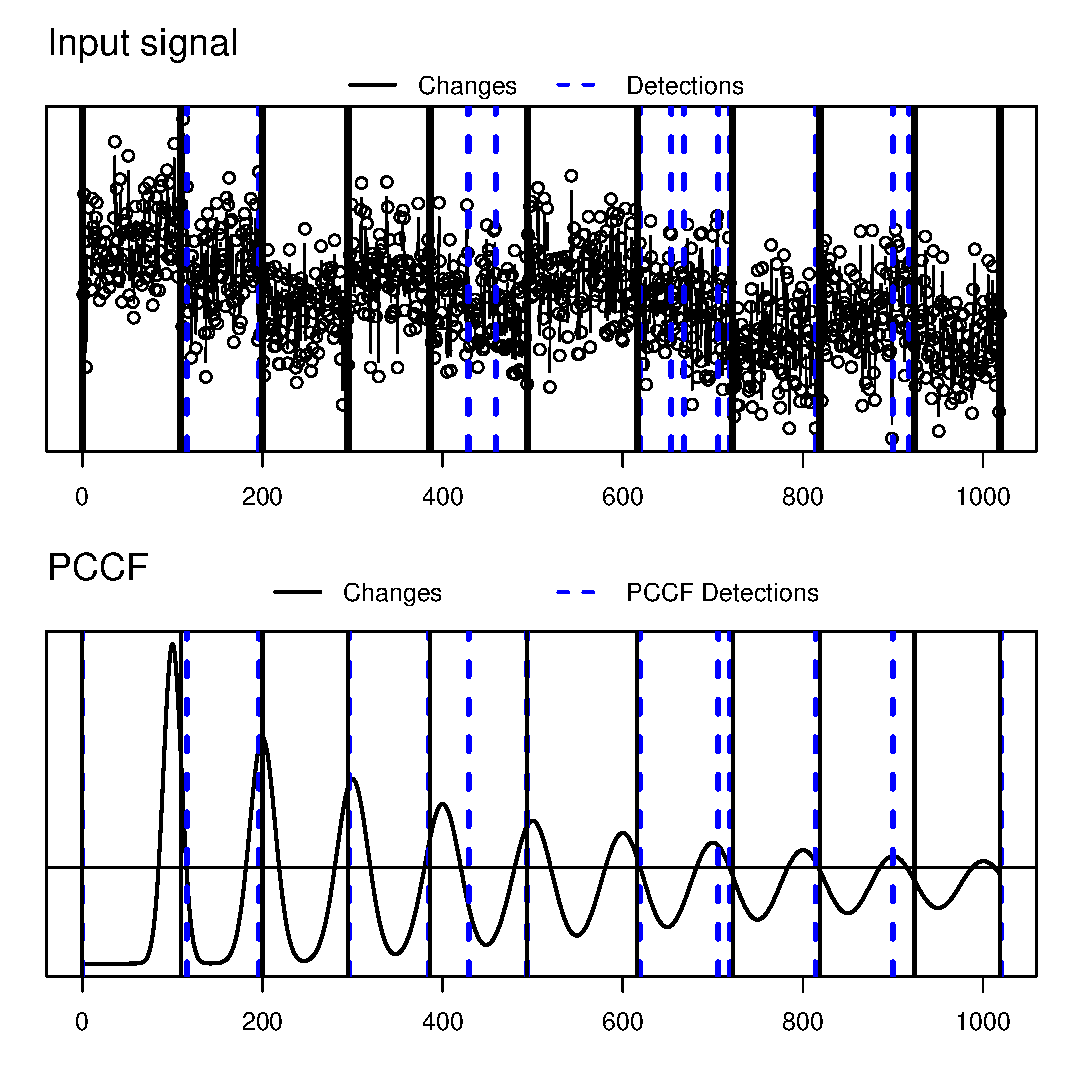
\includegraphics[width=0.8 \textwidth,
            trim={0.5cm 0cm 0.5cm 0cm}]{./images/blpa_article/fig3_concept_proof.eps}}
        \fbox{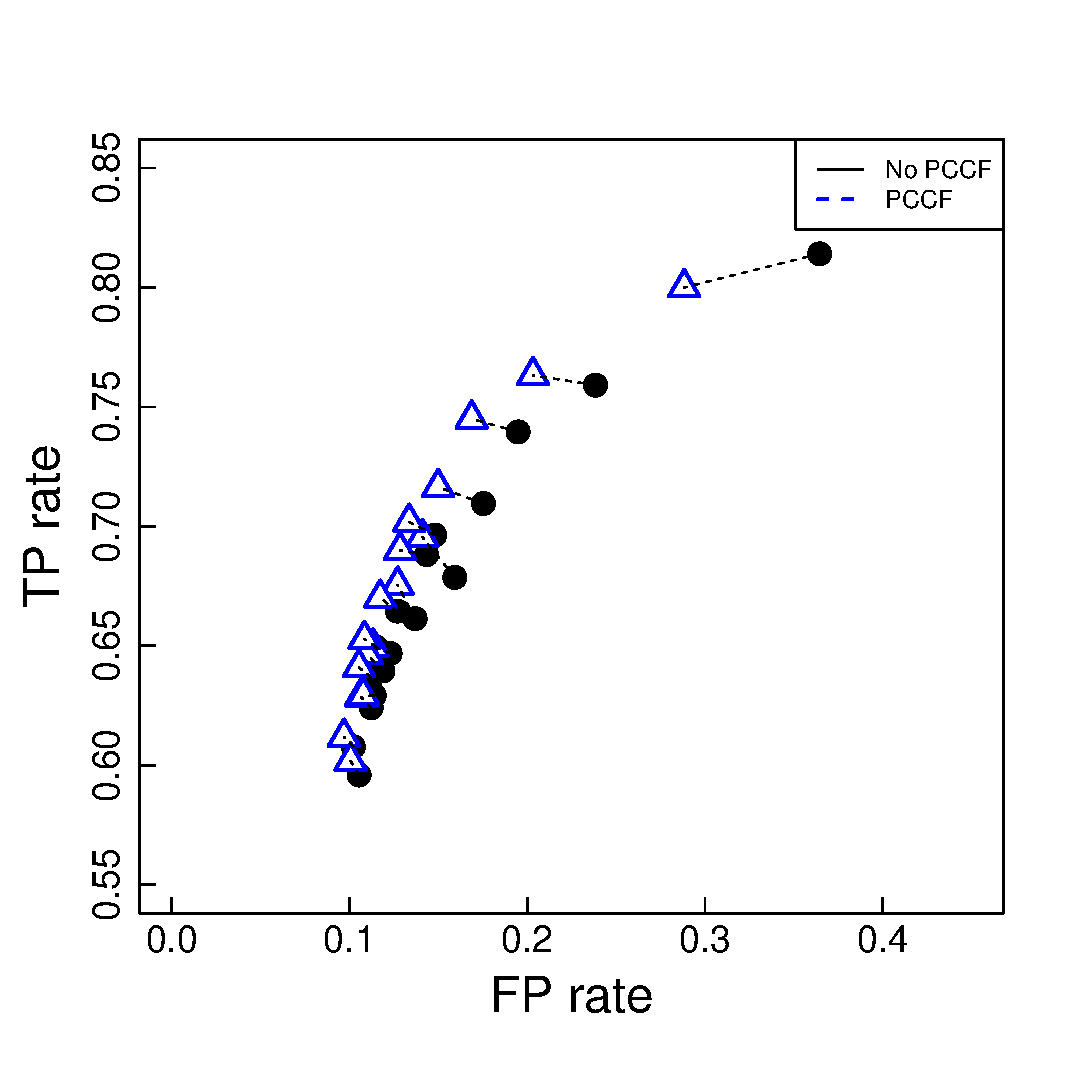
\includegraphics[
            width=0.787\textwidth,
            height = 0.27 \textheight,
            trim={0.0cm 1cm 1cm 1.7cm}]{./images/blpa_article/sim1_roc.eps}
            }
        \caption{
            Experimental results for simulated data streams with recurrent changes.
            On the top plot - an example of the generated input signal.
            %
            Vertical solid lines depict changepoints to be detected. 
            Dashed lines on the plot with the signal depict moments when detector \textbf{without} PCCF alarmed changes.
            %
            Bottom plot - ROC curves. 
            Blue triangles depict performance of the detector equipped with PCCF.
            Black dots - performance without PCCF.
            FP rate is reduced while keeping the same TP rate.
            }
            \label{fig:results1}
    \end{minipage}
\end{figure}
FP rate is decreased while not reducing TP rate.
In the worst cases the performance of both detectors is similar.

\subsection{Human Activity (HA) signal}
%https://archive.ics.uci.edu/ml/datasets/Smartphone-Based+Recognition+of+Human+Activities+and+Postural+Transitions
In the second experiment we used the Human activity data set~\cite{reyes2016transition} which contains sensor measurements from people performed 6 types of activities: three static postures (standing, sitting, lying) and three dynamic activities (walking, walking downstairs and walking
upstairs).
We detected changes in the signal caused by transitions from one set activities to another.
Results are depicted in Fig.~\ref{fig:results2}.
\begin{figure}[!htb]
%this is \input{FigResults2.tex}
    \begin{minipage}{0.5\textwidth}
        \centering
        \fbox{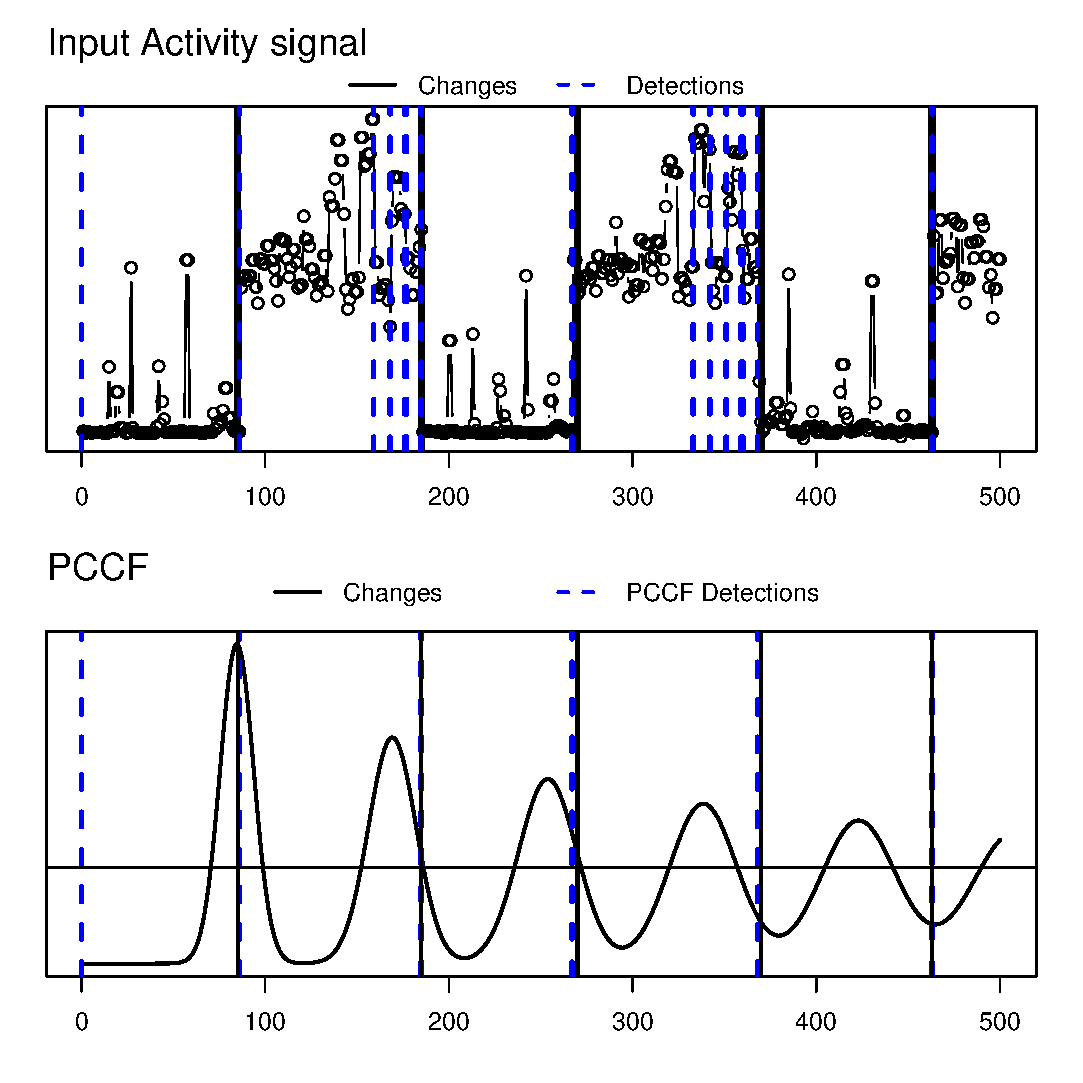
\includegraphics[width=0.8\textwidth, trim={0.5cm 0cm 0.5cm 0cm}]{./images/blpa_article/fig4_concept_proof_real.eps}}
        \\
        \fbox{
            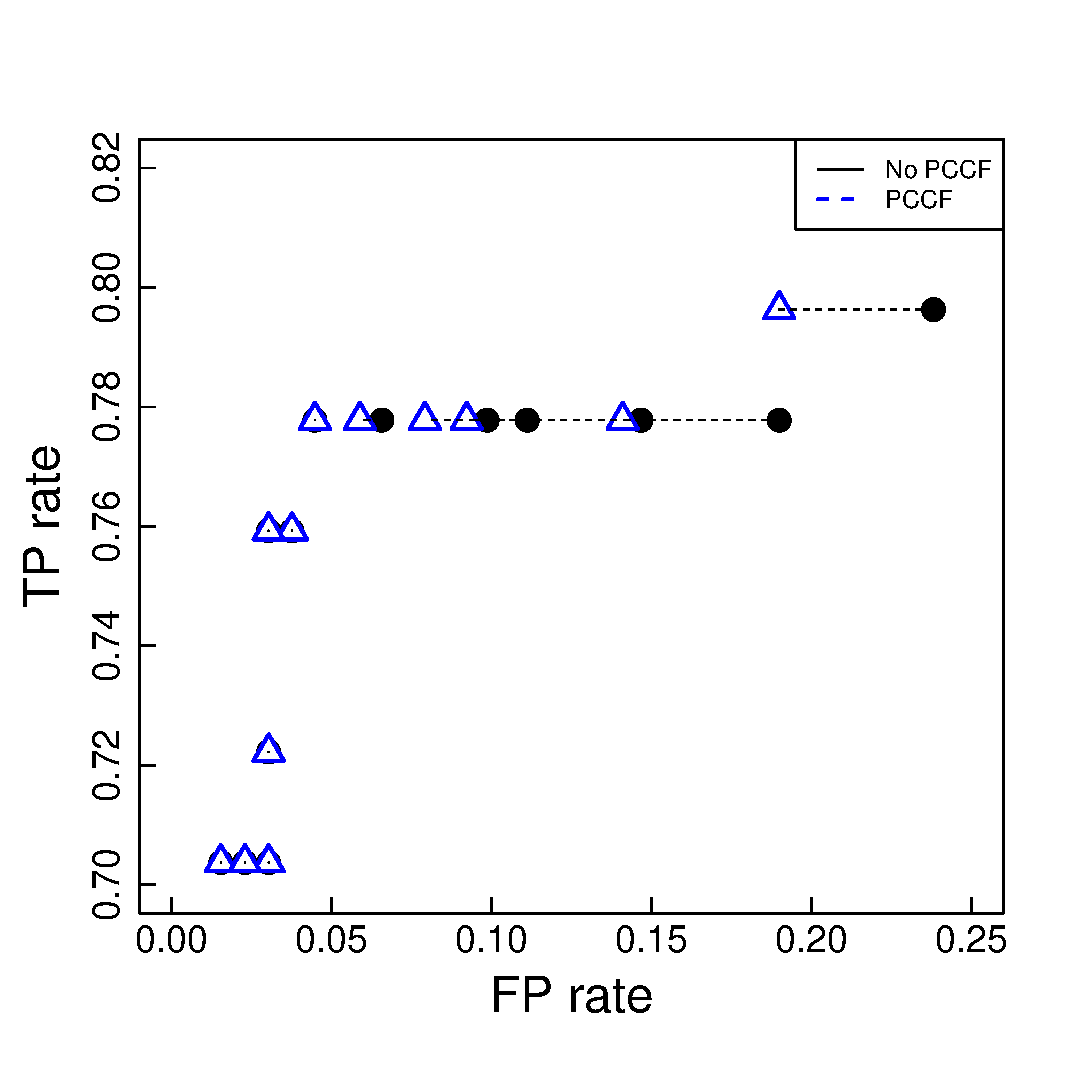
\includegraphics[
            width=0.773\textwidth, 
            height = 0.27 \textheight,
            trim={0.0cm 1cm 1cm 1.7cm}]{./images/blpa_article/exp1_roc_real.eps}
            }
        \caption{
         Experimental results for the 'Activity recognition' signal.
         On the top plot - illustrating example of the signal and corresponding PCCF function.
         Vertical solid lines depict changepoints to be detected. 
         Dashed lines on the plot with the signal depict moments when detector \textbf{without} PCCF alarmed changes. 
         Dashed lines on the plot \textbf{with} PCCF show time moments when the detector with PCCF alarmed changes.
         Bottom plot - ROC curves. 
        Blue triangles - performance of the BD with PCCF.
            }
            \label{fig:results2}
    \end{minipage}
\end{figure}
FP rate is decreased when BD detector is used with the PCCF function.


\section{Conclusion}
We proposed the method to improve performance of the Bayesian Online Changepoint detector (BD) for the data streams with recurrent changes by embedding into it the Predictive Confidence Change Function (PCCF).
%
While observing a new data both BD detector's and PCCF's parameters are adjusted in a uniform way to the changing conditions using the same Bayesian update procedures constituting a two-layer adaptive change detection/prediction method BLPA.
%
In the experiments with real and artificial data sets we demonstrated that Bayesian detector equipped with PCCF performs better in terms of TP/FP rates than the detector without PCCF.
%We extended the method proposed in~\cite{mackay2007} by
%\bibliographystyle{IEEEtran}
%\input{./parts/Appendix}
\appendix
\noindent
\textbf{Marginal predictive distribution} $p(x_{n+1}|x_1,...,x_n)$ can be found as
\begin{align}
\label{eq:post1}
    &p(x_{n+1}|x_1,...,x_n)\\\nonumber
    &=\frac{ \int_{\tau\in \mathbb{R}^+} \int_{\mu\in \mathbb{R}}p(x_1,....,x_{n+1}|\mu,\tau) p(\mu,\tau)d\mu d\tau}{ \int_{\tau\in \mathbb{R}^+} \int_{\mu\in\mathbb{R}}p(x_1,....,x_{n}|\mu,\tau) p(\mu,\tau)d\mu d\tau}.
\end{align}
Assuming the Gaussian distribution 
\begin{equation}
    p(x|\mu,\tau)=\frac{\sqrt{\tau}}{\sqrt{2\pi}} e^{-\frac{\tau}2 (x-\mu)^2}
    \label{eq:gauss_appendix}
\end{equation}
the probability $p(x_1,....,x_{n}|\mu,\tau) p(\mu,\tau)$ is
\begin{align}\label{eq:prob1}
    \left(\frac{\sqrt{\tau}}{\sqrt{2\pi}}\right)^{n}\times &\exp\left(-\frac{\tau}{2}\sum_{i=1}^{n} (x_i-\mu)^2\right) \tau^{\alpha_0-1/2}\\\nonumber &\times\exp\left(-\frac{\tau}2 \left(\kappa_0(\mu-\mu_0)^2+2\beta_0\right) \right)
\end{align}
where an expression in the exponent is 
\begin{align}
    &-\frac{\tau(n+\kappa_0)}{2}\sum_{i=1}^{n} \left(\mu-\frac{\sum_{i=1}^{n} x_i+\mu_0 \kappa_0}{n+\kappa_0}\right)^2\\\nonumber &-\frac{\tau}{2} \left(\sum_{i=1}^{n} x_i^2 + \kappa_0\mu_0^2 - \frac{(\sum_{i=1}^{n}x_i +\mu_0 \kappa_0)^2}{n+\kappa_0}+2\beta_0\right),
\end{align}
Therefore %from where
\begin{align}
    &p(x_1,....,x_{n}|\mu,\tau) p(\mu,\tau)\\\nonumber
    =& \left(\frac{1}{\sqrt{2\pi}}\right)^{n-1} \frac{\Gamma(\alpha_0+n/2)}{\sqrt{n+\kappa_0}} \left(\frac{\hat{b}_n}2\right)^{-\alpha_0+n/2}\\\nonumber \times &\GammaDistr(\tau|\alpha_0+n/2,\hat{a}_n/2) \mathcal{N}(\mu|\hat{\mu}_n,\hat{\sigma}^2_n)
\end{align}
where posterior parameters estimates $\hat{a}_n, \hat{\mu}_n, \hat{\sigma}^2_n$ are
\begin{align}
    &\hat{a}_n = \left(\sum_{i=1}^{n} x_i^2 + \kappa_0\mu_0^2 - \frac{(\sum_{i=1}^{n}x_i +\mu_0 \kappa_0)^2}{n+\kappa_0}+2\beta_0\right),\\\nonumber &\hat{\mu}_n = \frac{\sum_{i=1}^{n}x_i+\mu_0 \kappa_0}{n+\kappa_0},\ \hat{\sigma}^2_n = \frac{1}{\tau(n+\kappa_0)}.
\end{align}
Therefore the integral in the numerator in Equation~\ref{eq:post1} is
\begin{align}
    &\int_{\tau\in \mathbb{R}^+} \int_{\mu\in \mathbb{R}}p(x_1,....,x_{n+1}|\mu,\tau) p(\mu,\tau)d\mu d\tau\\\nonumber
    =& \left(\frac{1}{\sqrt{2\pi}}\right)^{n-1} \frac{\Gamma(\alpha_0)}{\sqrt{n+\kappa_0}} \left(\frac{\hat{a}_n}2\right)^{-(\alpha_0+n/2)}
\end{align}
and integral~\ref{eq:post1} can be expressed as
\begin{align}
    &\frac{\sqrt{n+\kappa_0}}{\sqrt{n+1+\kappa_0}\ B(\alpha_0+n/2,1/2)} \frac{\hat{a}_n^{\alpha_0+n/2}}{\hat{a}_{n+1}^{\alpha_0+(n+1)/2}}\\\nonumber
    =&\frac{\sqrt{n+\kappa_0}}{\sqrt{n+1+\kappa_0}\ B(\alpha_0+n/2,1/2)} \left(\frac{\hat{a}_{n+1}}{\hat{a}_n}\right)^{-(\alpha_0+(n+1)/2)} \hat{a}_n^{-1/2}.
\end{align}
Noticing that
\begin{align}
    &\frac{\hat{a}_{n+1}}{\hat{a}_n} = 1+ \frac{n+\kappa_0}{\hat{a}_n(n+1+\kappa_0)}\\\nonumber \times &\left(x_{n+1}^2 - \frac{2x_{n+1}\left(\sum_{i=1}^n x_i +\mu_0 \kappa_0\right)}{n+\kappa_0}
    + \frac{\left(\sum_{i=1}^n x_i +\mu_0 \kappa_0\right)^2}{(n+\kappa_0)^2}\right)
\end{align}
\textbf{marginal predictive distribution} is 
\begin{align}
    &p(x_{n+1}|x_1,...,x_n)\\\nonumber =& \frac{1}{\hat{b}_n B(\alpha_0+n/2,1/2)} \left(
1+\frac{(x_{n+1}-\lambda)^2}{\hat{b}_n^2}\right)^{-(\alpha_0+(n+1)/2)},
\end{align}
where coefficients are
\begin{equation}
    \hat{b}_n = \frac{\sqrt{(n+1+\kappa_0)\hat{a}_n}}{\sqrt{(n+\kappa_0)}},\ \lambda = \frac{\sum_{i=1}^n x_i +\mu_0 \kappa_0}{n+\kappa_0}.
\end{equation}




\chapter{Refs}
\begin{itemize}
  \item Change detection:~\cite{basseville1993detection}
  \item Sequential change detection problem is a well studied problem, see for example in~\cite{tartakovsky2014sequential},~\cite{plasse2021streaming}.

  \item Optimality of the change detection procedure was investigated in~\cite{Page1954},~\cite{Shiryaev2010,Shiryaev1961,Shiryaev1963}.
  Asymptotic and nonasymptotic optimality of cumulative sum algorithms was provedin~\cite{lorden1971procedures},~\cite{moustakides1986optimal},~\cite{moustakides2004optimality},~\cite{ritov1990decision}. In~\cite{Shiryaev1963,shiryaev2007optimal} the change point is modelled as a random variable with a known geometric distribution~\cite{veeravalli2014quickest} and optimal algorithm minimizing the average detection delay given constraint on the probability of false alarm is proposed. In our work we minimize the detection delay given a constraint on the maximum delay imposed by the prediction interval width. In~\cite{lorden1971procedures} asymptotic optimality of Cusum~\cite{Page1954} is proved according to the minimax criterion for delay with the mean time between false alarms going to infinity.

  \item Concept drift:
\end{itemize}

\tailmatter
\finnishsummary
Foo bar
%\inputencoding{utf8}
\bibliographystyle{apalike}
\bibliography{references}
\bibliography{references_cfb}
\bibliography{references_ijcnn}
\bibliography{references_aclac}
\appendices
\appendix{A}
\section{foobar}

\backmatter

\includedarticles
\begin{article}{sha1}
	\arttitle{Modelling Recurrent Events for Improving Online Change Detection}
	\artauthor{Alexandr Maslov, Mykola Pechenizkiy, Indr{\.e} {\v{Z}}liobait{\.e}, and Tommi K\"{a}rkk\"{a}inen}
	\artpublish{Proceedings of the 2016 SIAM International Conference on Data Mining}
	\artyear{2016}
	\artcopyright{XX}
	\artpages{1}
\end{article}

\begin{article}{sha2}
	\arthide
	\arttitle{BLPA: Bayesian learn-predict-adjust method for online detection of recurrent changepoints}
	\artauthor{Alexandr  Maslov, Mykola Pechenizkiy, Yulong  Pei, Indre {\v{Z}}liobait{\.e},  Alexander Shklyaev, Tommi Karkk{\"a}inen, and Hollm{\'e}n, Jaakko}
	\artpublish{2017 International Joint Conference on Neural Networks (IJCNN)}
	\artyear{2017}
	\artcopyright{XXX}
\end{article}
\printindex
\end{document}
